%%%%%%%%%%%%%%%%%%%%%%%%%%%%%%%%%%%%%%%%%%%%%%%%%%%%%%%%%%%
\documentclass[xcolor=x11names,compress]{beamer}
%\documentclass[xcolor=x11names,compress, handhouts, aspectratio=169]{beamer}
%% General document
\usepackage{graphicx, subfig}
%% Beamer Layout
\useoutertheme[subsection=false,shadow]{miniframes}
\useinnertheme{default}
\usefonttheme{serif}
\usepackage{palatino}

%%%%%%% Mes Packages %%%%%%%%%%%%%%%%
%\usepackage[french]{babel}
\usepackage[T1]{fontenc}
\usepackage{color}
\usepackage{xcolor}
\usepackage{dsfont} % Pour indicatrice
\usepackage{url}
\usepackage{multirow}
\usepackage[normalem]{ulem}   % For strike out text

% Natbib for clean bibliography
\usepackage[comma,authoryear]{natbib}

%remove the icon
\setbeamertemplate{bibliography item}{}

%remove line breaks
\setbeamertemplate{bibliography entry title}{}
\setbeamertemplate{bibliography entry location}{}
\setbeamertemplate{bibliography entry note}{}

%% ------ MEs couleurs --------
\definecolor{vert}{rgb}{0.1,0.7,0.2}
\definecolor{brique}{rgb}{0.7,0.16,0.16}
\definecolor{gris}{rgb}{0.7, 0.75, 0.71}
\definecolor{twitterblue}{rgb}{0, 0.42, 0.58}
\definecolor{airforceblue}{rgb}{0.36, 0.54, 0.66}
\definecolor{siap}{RGB}{3,133, 200}


%%%%%%%%%%%%%%%%% BEAMER PACKAGE %%%%%%%

\setbeamercolor{itemize item}{fg=siap}
%\setbeamercolor{itemize subitem}{fg=blue}
%\setbeamercolor{itemize subsubitem}{fg=cyan}

\setbeamerfont{title like}{shape=\scshape}
\setbeamerfont{frametitle}{shape=\scshape}

\setbeamercolor*{lower separation line head}{bg=DeepSkyBlue4}
\setbeamercolor*{normal text}{fg=black,bg=white}
\setbeamercolor*{alerted text}{fg=siap}
\setbeamercolor*{example text}{fg=black}
\setbeamercolor*{structure}{fg=black}
\setbeamercolor*{palette tertiary}{fg=black,bg=black!10}
\setbeamercolor*{palette quaternary}{fg=black,bg=black!10}

% Set the header color to SIAP's color
\setbeamercolor*{frametitle}{fg=siap}

%remove navigation symbols
\setbeamertemplate{navigation symbols}{}

\renewcommand{\(}{\begin{columns}}
\renewcommand{\)}{\end{columns}}
\newcommand{\<}[1]{\begin{column}{#1}}
\renewcommand{\>}{\end{column}}

%% Add footer with logo
\setbeamertemplate{footline}{%
  \begin{beamercolorbox}[wd=\paperwidth,ht=2.5ex,dp=1.125ex,%
    leftskip=.3cm,rightskip=.3cm plus1fil]{author in head/foot}
    
\includegraphics[height=5ex]{SIAP-ESCAP-Logo.png}\hfill
    \insertshortauthor\hfill\insertshorttitle\hfill  \textcolor{siap}{\textit{\insertframenumber}}
  \end{beamercolorbox}%
}

% Path for the graphs
\graphicspath{
{Graphics/}
%{c:/Chris/UN-ESCAP/SIAP-E-learning/Resources/OpenScience/}
%{c:/Chris/Visualisation/Presentations/Graphics/}
%{c:/Chris/Visualisation/Presentations/Graphics/SIAP/}
%{c:/Chris/Visualisation/Presentations/Graphics/Lies/}
%{c:/Chris/Visualisation/Presentations/Graphics/Maps/}
%{c:/Chris/Visualisation/Presentations/Graphics/RGenerated/}
%{c:/Chris/Visualisation/Presentations/Graphics/Logos/}
%{c:/Gitmain/MLCourse/UNML/Module0/M0_files/figure-html/}
%{c:/Chris/UN-ESCAP/MyCourses2022/MLOS2022/Slides/Graphics/}
%{c:/Chris/UN-ESCAP/MyCourses2023/RAP/Slides/Graphics/}
%{c:/GitMain/RAP/RAP-Course/images/}
%{c:/Chris/UN-ESCAP/MyCourses2022/MLOS2022/Slides/Graphics/}
%% Path for specific graphs created
% {../R-Codes/JobSatisfaction_files/figure-latex/}
% {../R-Codes/Unused_files/figure-latex/}
 }


\title{\textcolor{siap}{Training on Web Scraping Prices for CPI \\ \vspace{0.5cm} }}

\subtitle{\textcolor{brique}{\Large{ Reproducible Analytical Pipelines}}}
\author{Christophe Bontemps \& Serge Goussev }
\institute{ 
\includegraphics[height=9ex]{SIAP-ESCAP-Logo.png} \hspace{1cm} 
\includegraphics[height=10ex]{StatCanada-Logo.jpg}}
\date{}

\begin{document}

\section{Motivation}

\begin{frame}
  \titlepage
\end{frame}

\begin{frame}{Fundamental Principles of Official Statistics}
  \begin{columns}[T]
    \begin{column}{0.6\textwidth}
      \begin{itemize}[<+->]
        \item Clear mention of the \textbf{processes} used to produce statistics
        \item \emph{To retain trust in official statistics, the \textbf{statistical agencies need to decide} according to strictly professional considerations, including scientific principles and professional ethics, \textbf{on the methods and procedures} for the collection, processing, storage and presentation of statistical data.}
      \item In short, \textbf{processes} are important!
      \end{itemize}
    \end{column}
    \begin{column}{0.4\textwidth}
      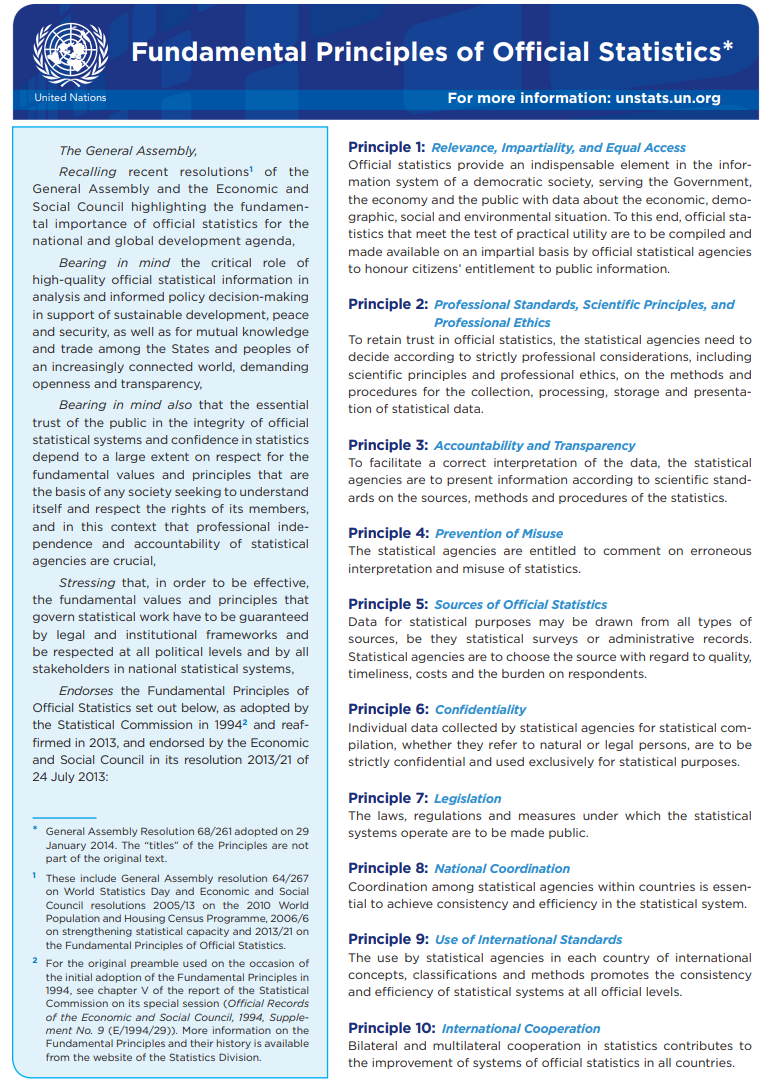
\includegraphics[width=\textwidth]{FundamentalPrinciplesOS.PNG}
    \end{column}
  \end{columns}
\end{frame}

\begin{frame}{Usual practice: Theory vs reality}
\begin{center}
  \begin{itemize}
        \only<1>{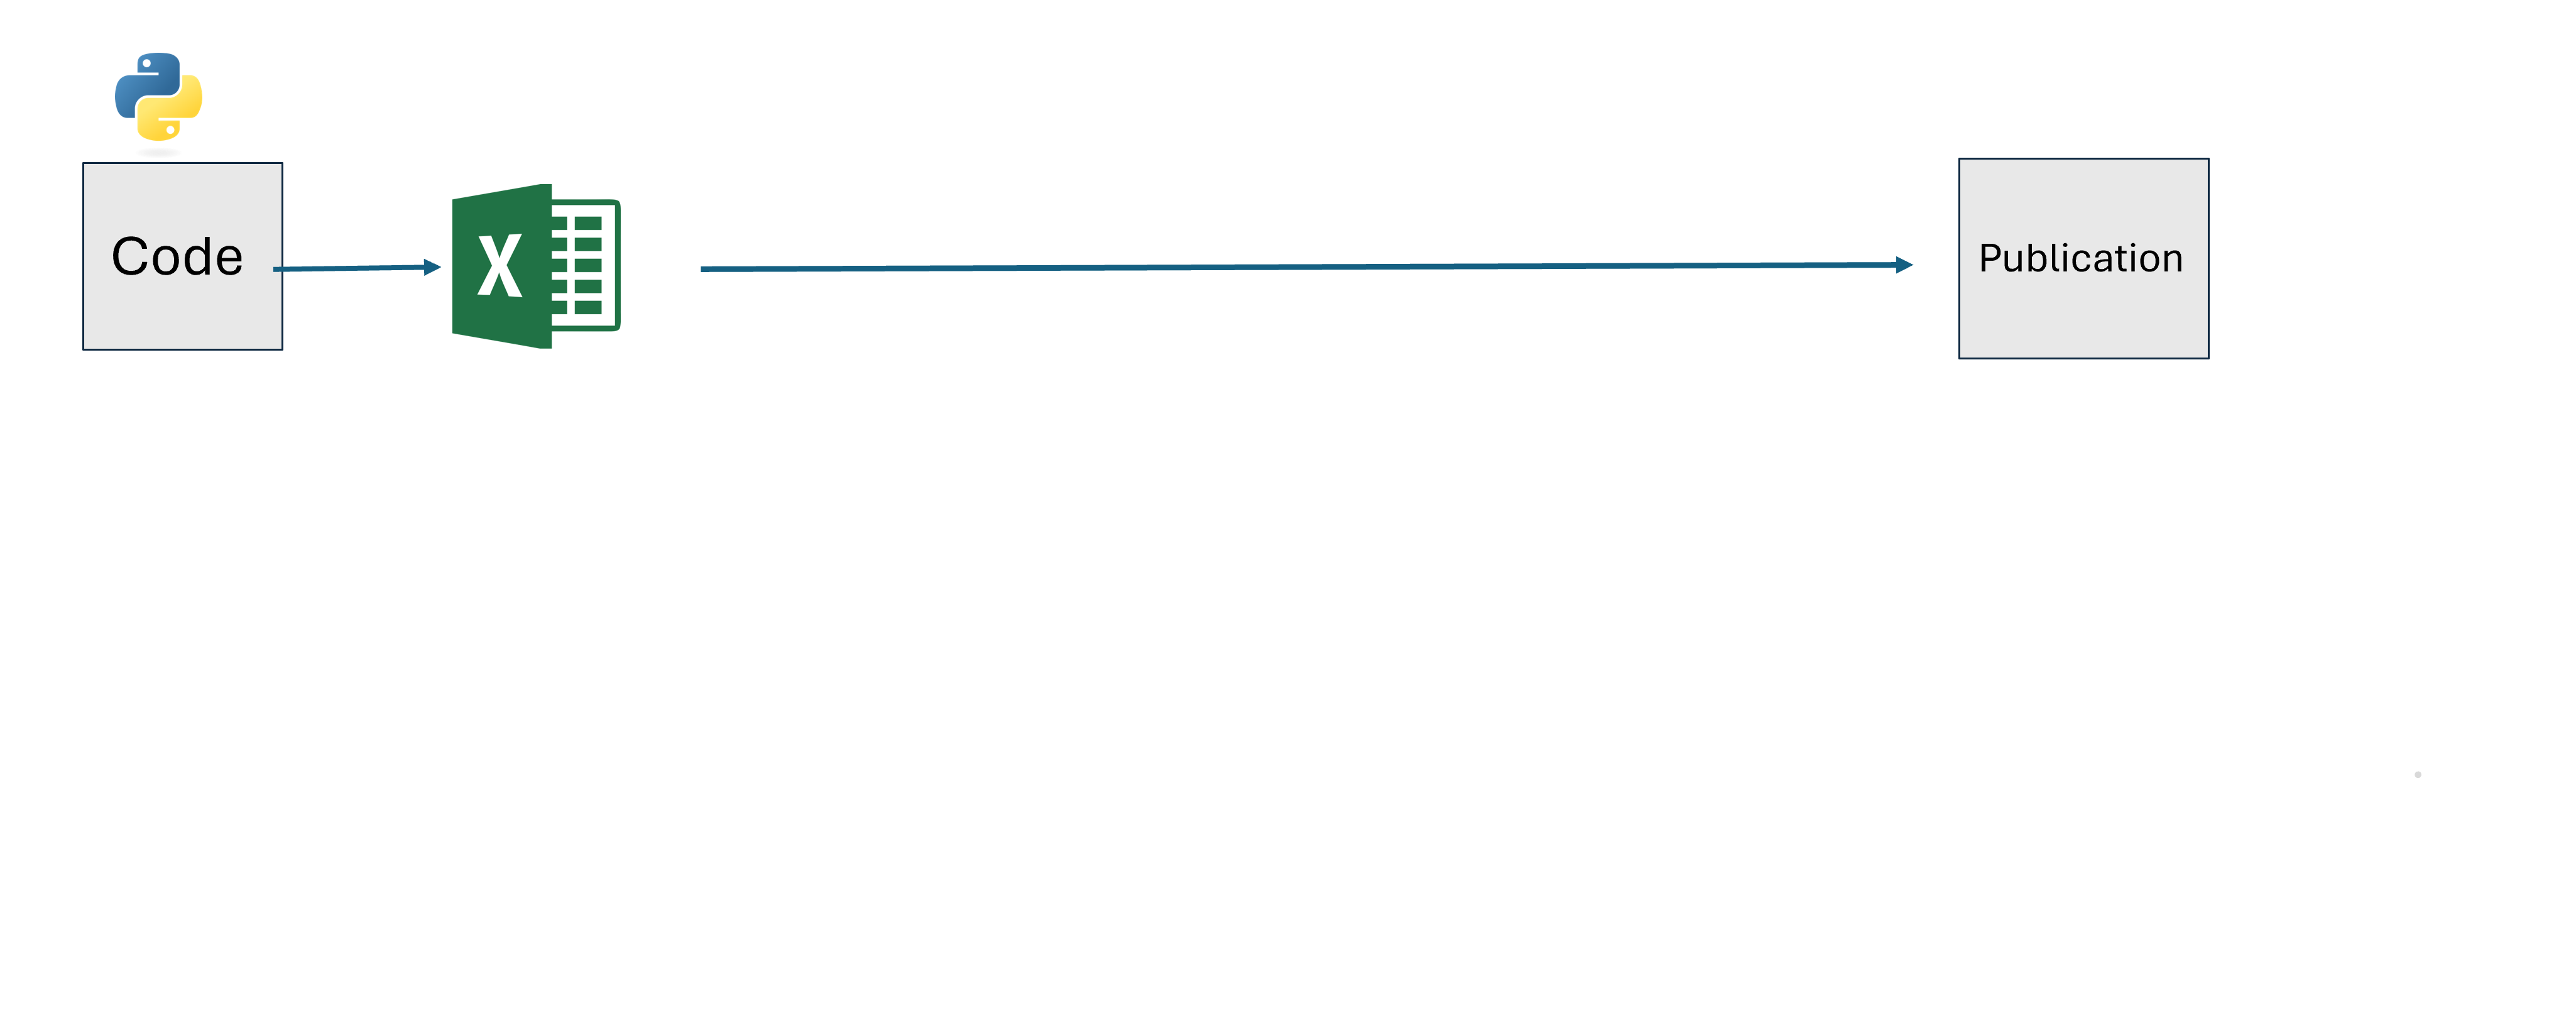
\includegraphics[width=0.8\textwidth]{Process1.png} \\ Comment 1}
        \only<2>{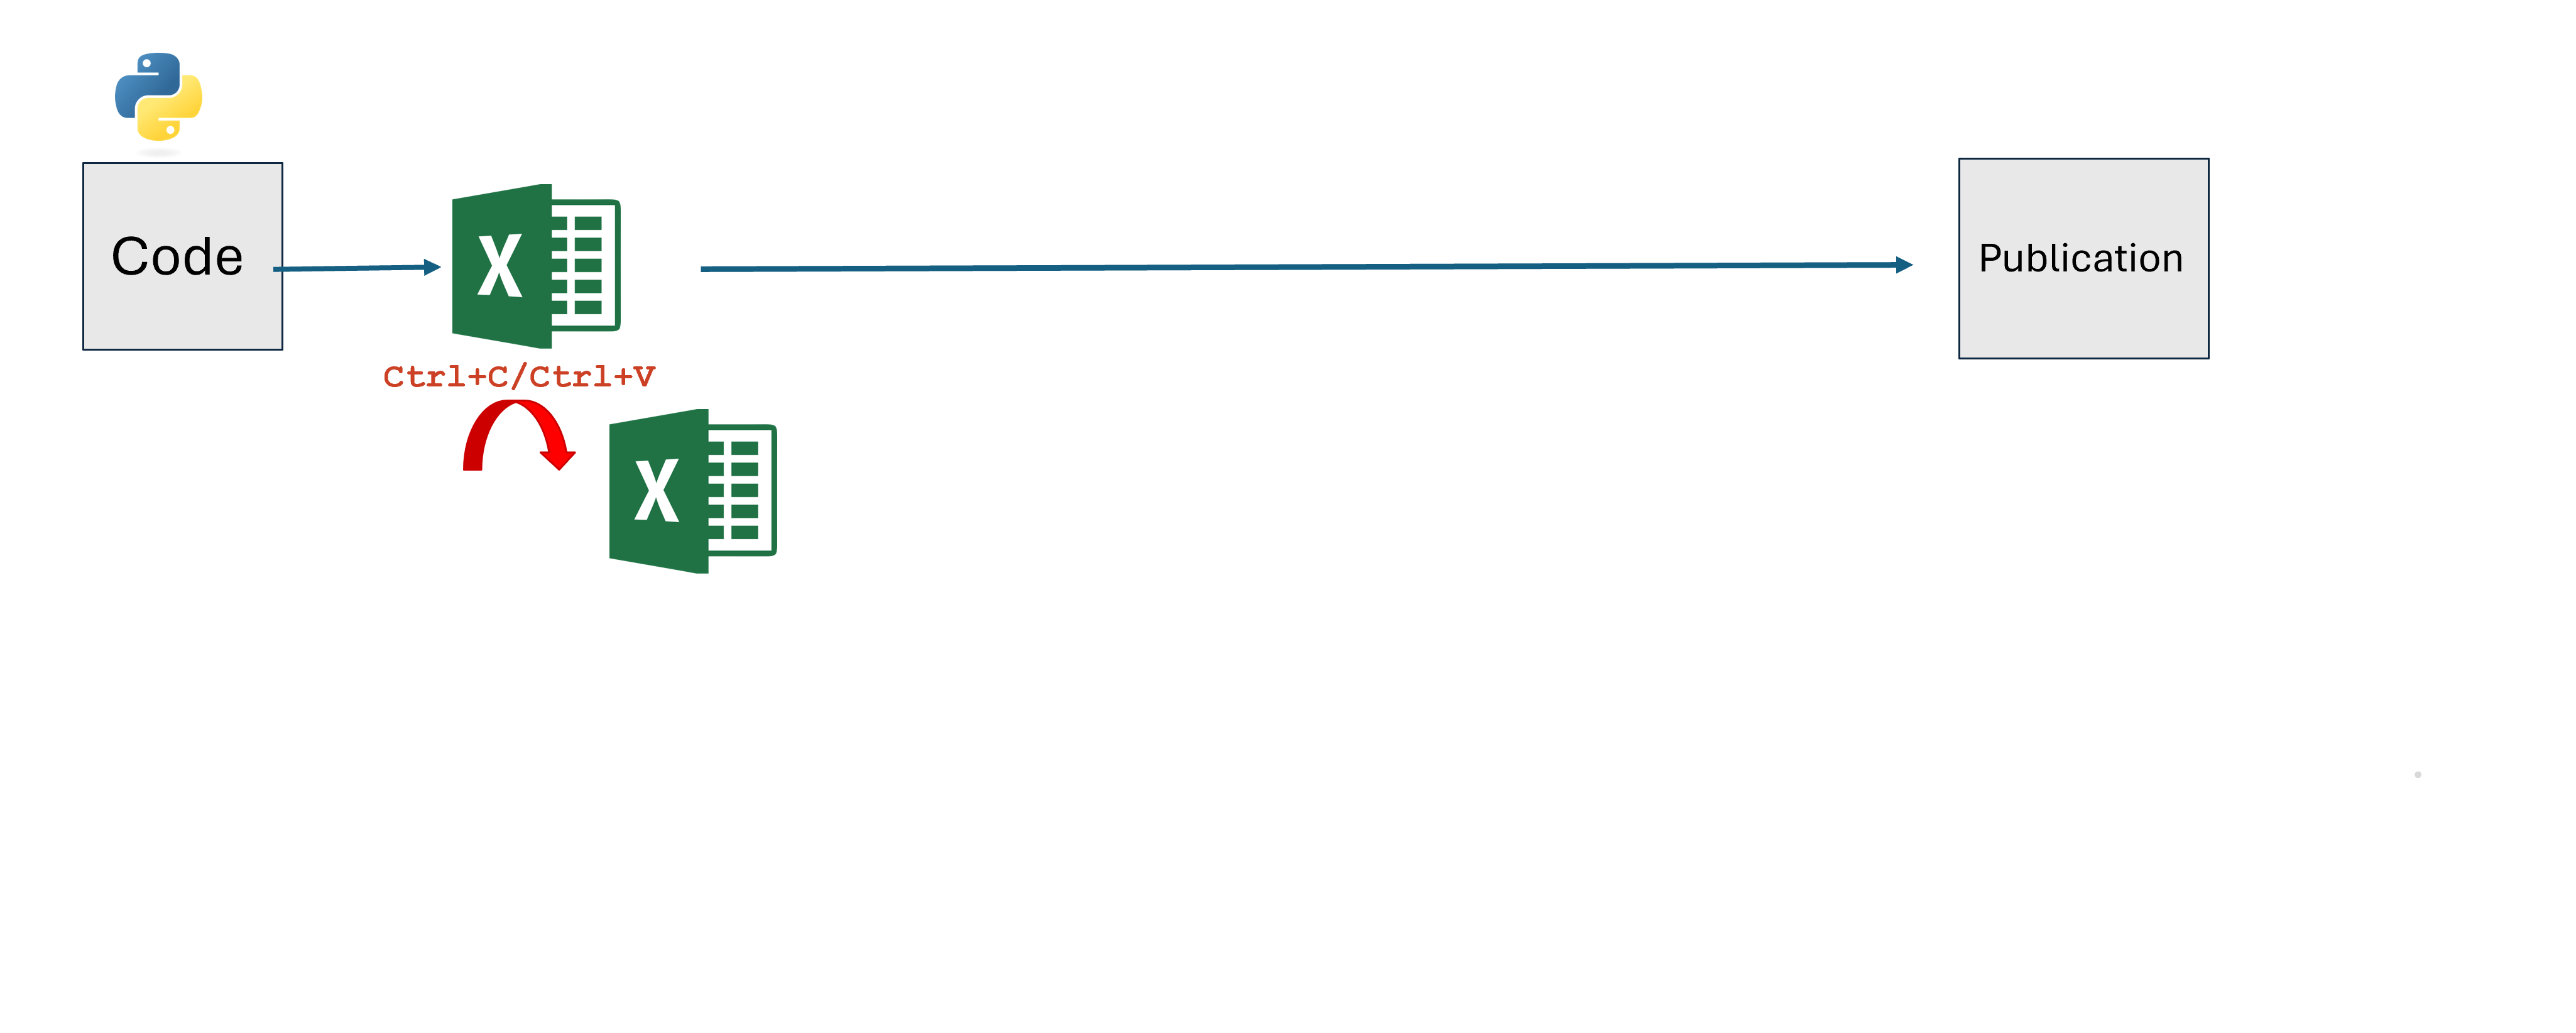
\includegraphics[width=0.8\textwidth]{Process2.png} \\ Comment 2}
        \only<3>{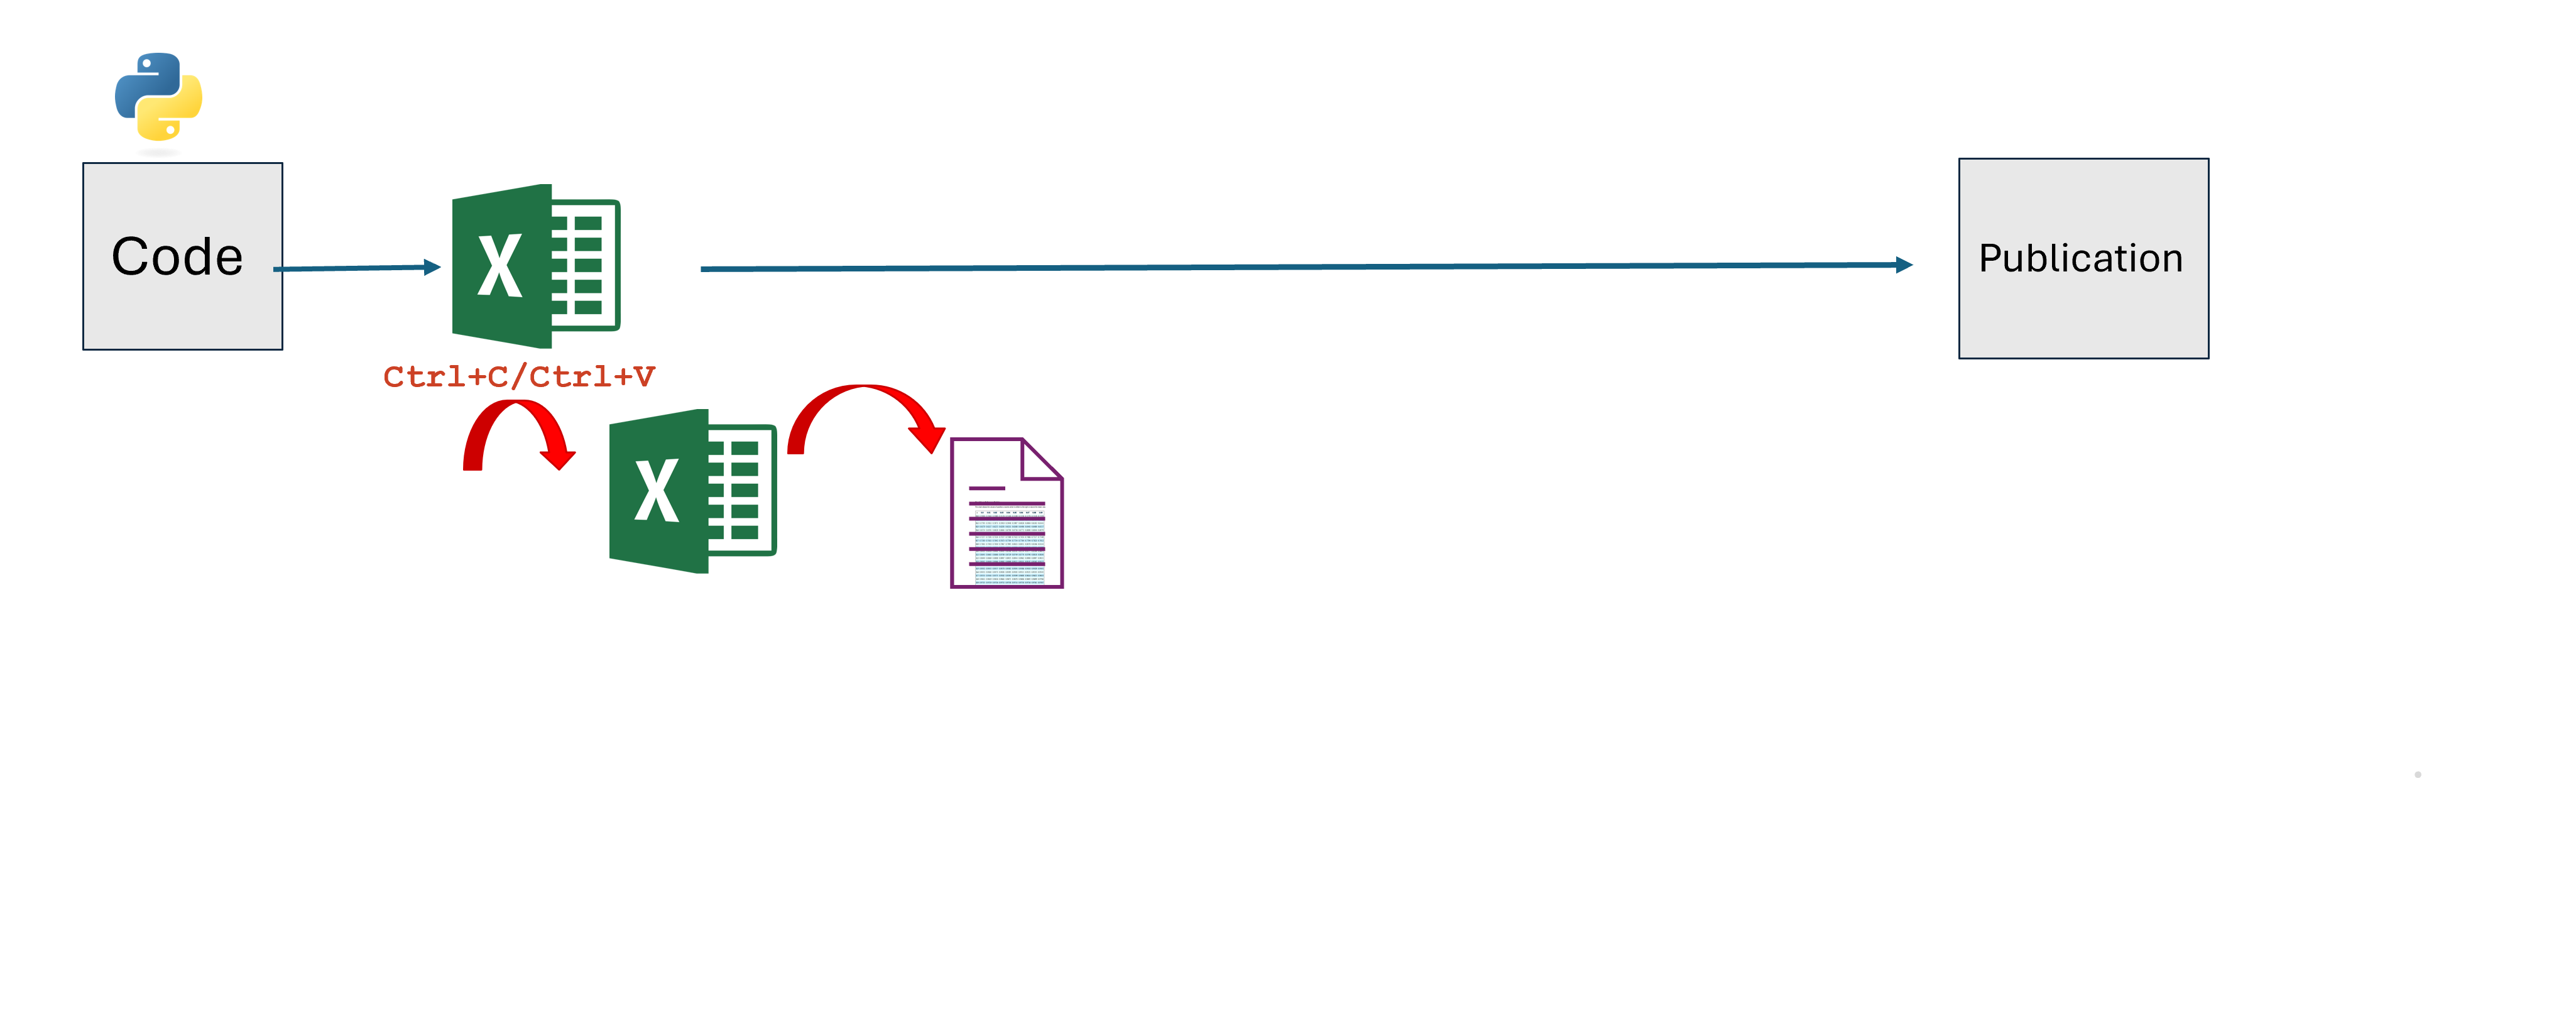
\includegraphics[width=0.8\textwidth]{Process3.png} \\ Comment 3}
        \only<4>{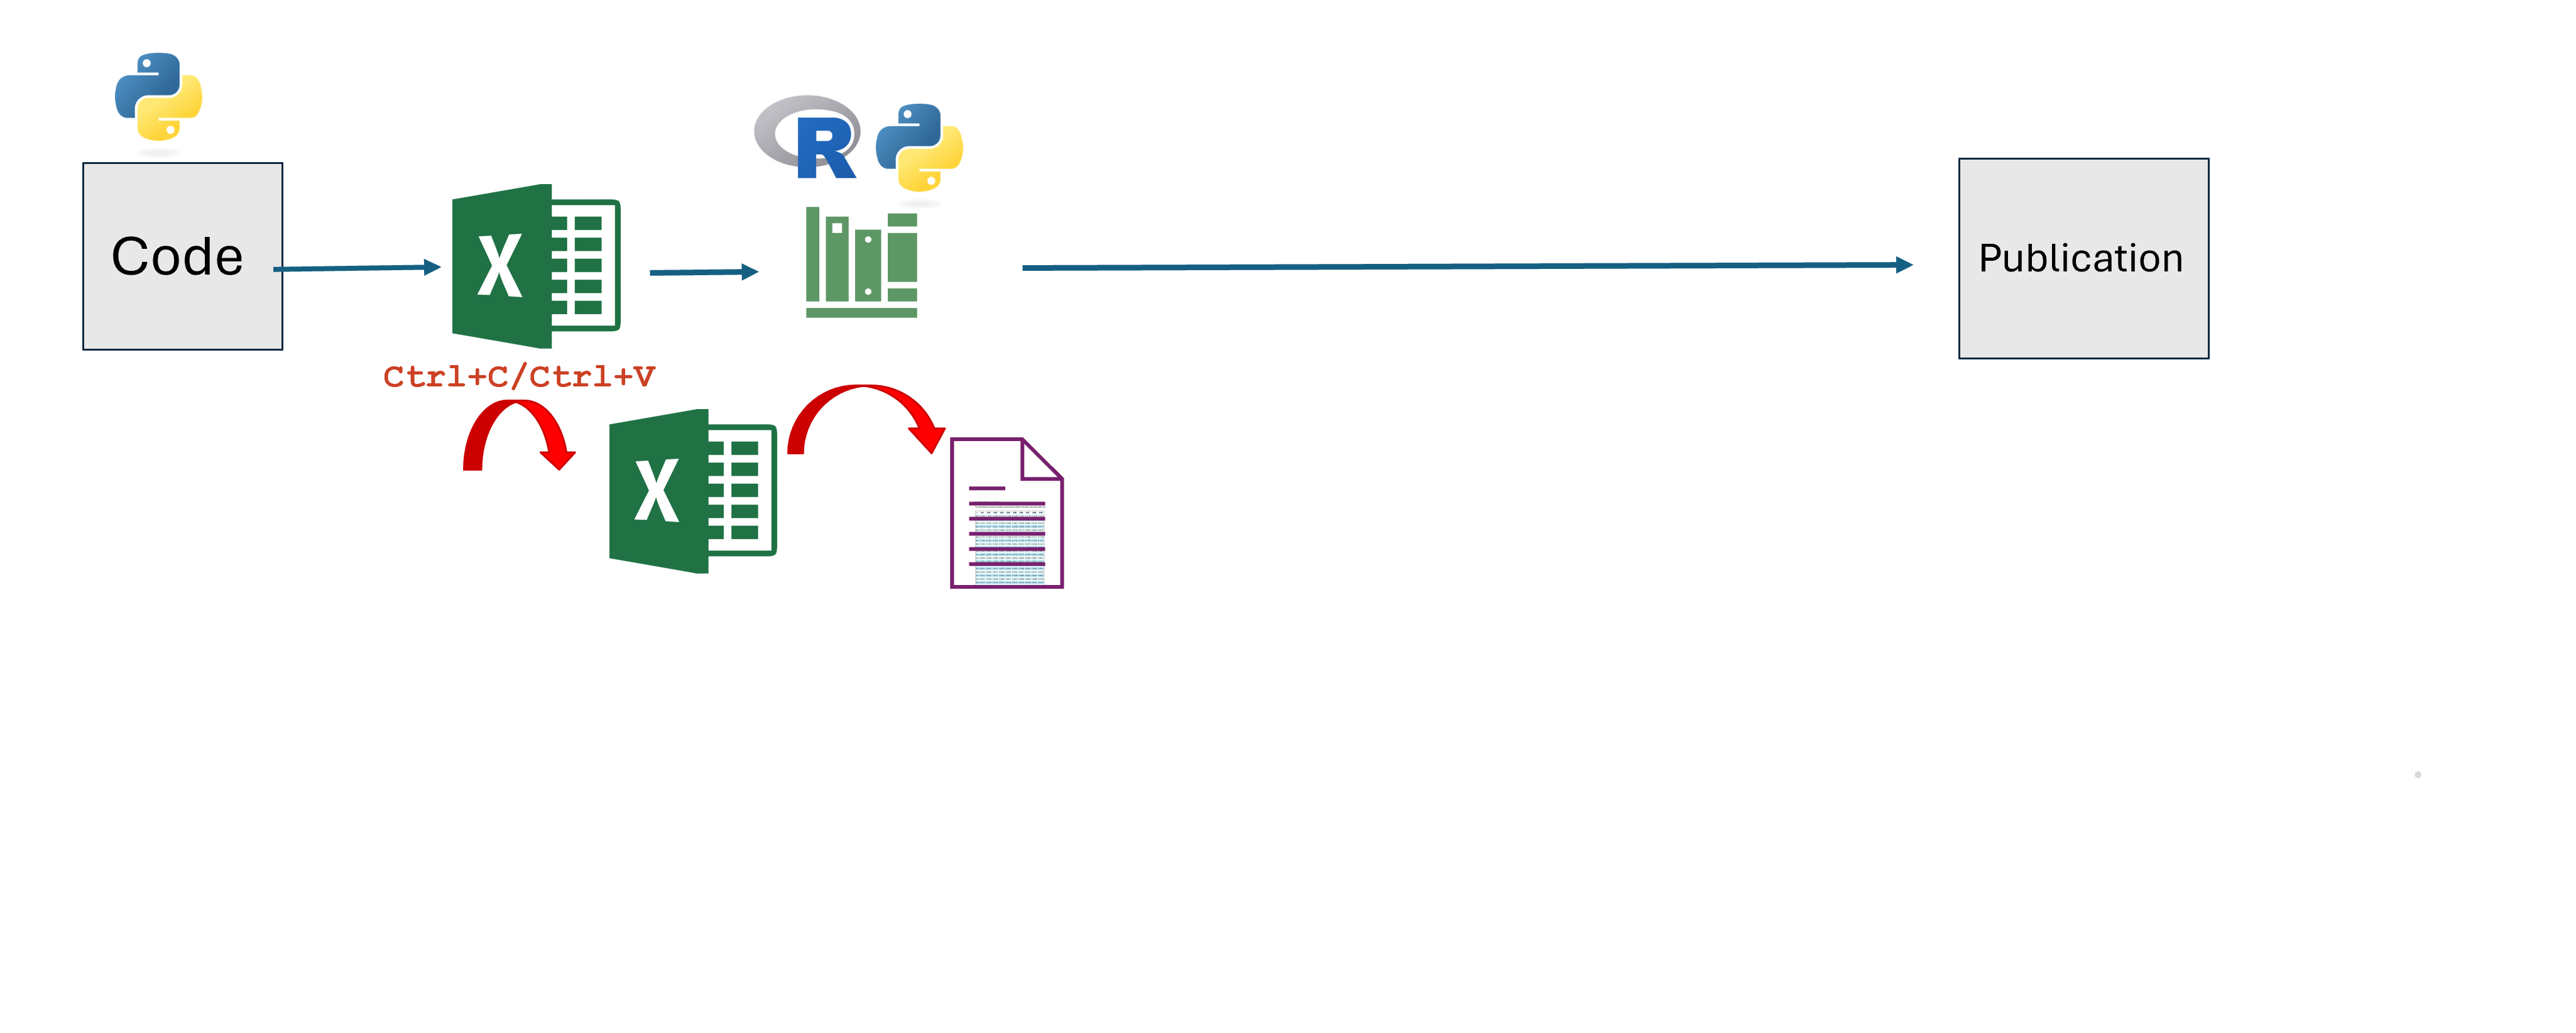
\includegraphics[width=0.8\textwidth]{Process4.png} \\ Comment 4}
        \only<5>{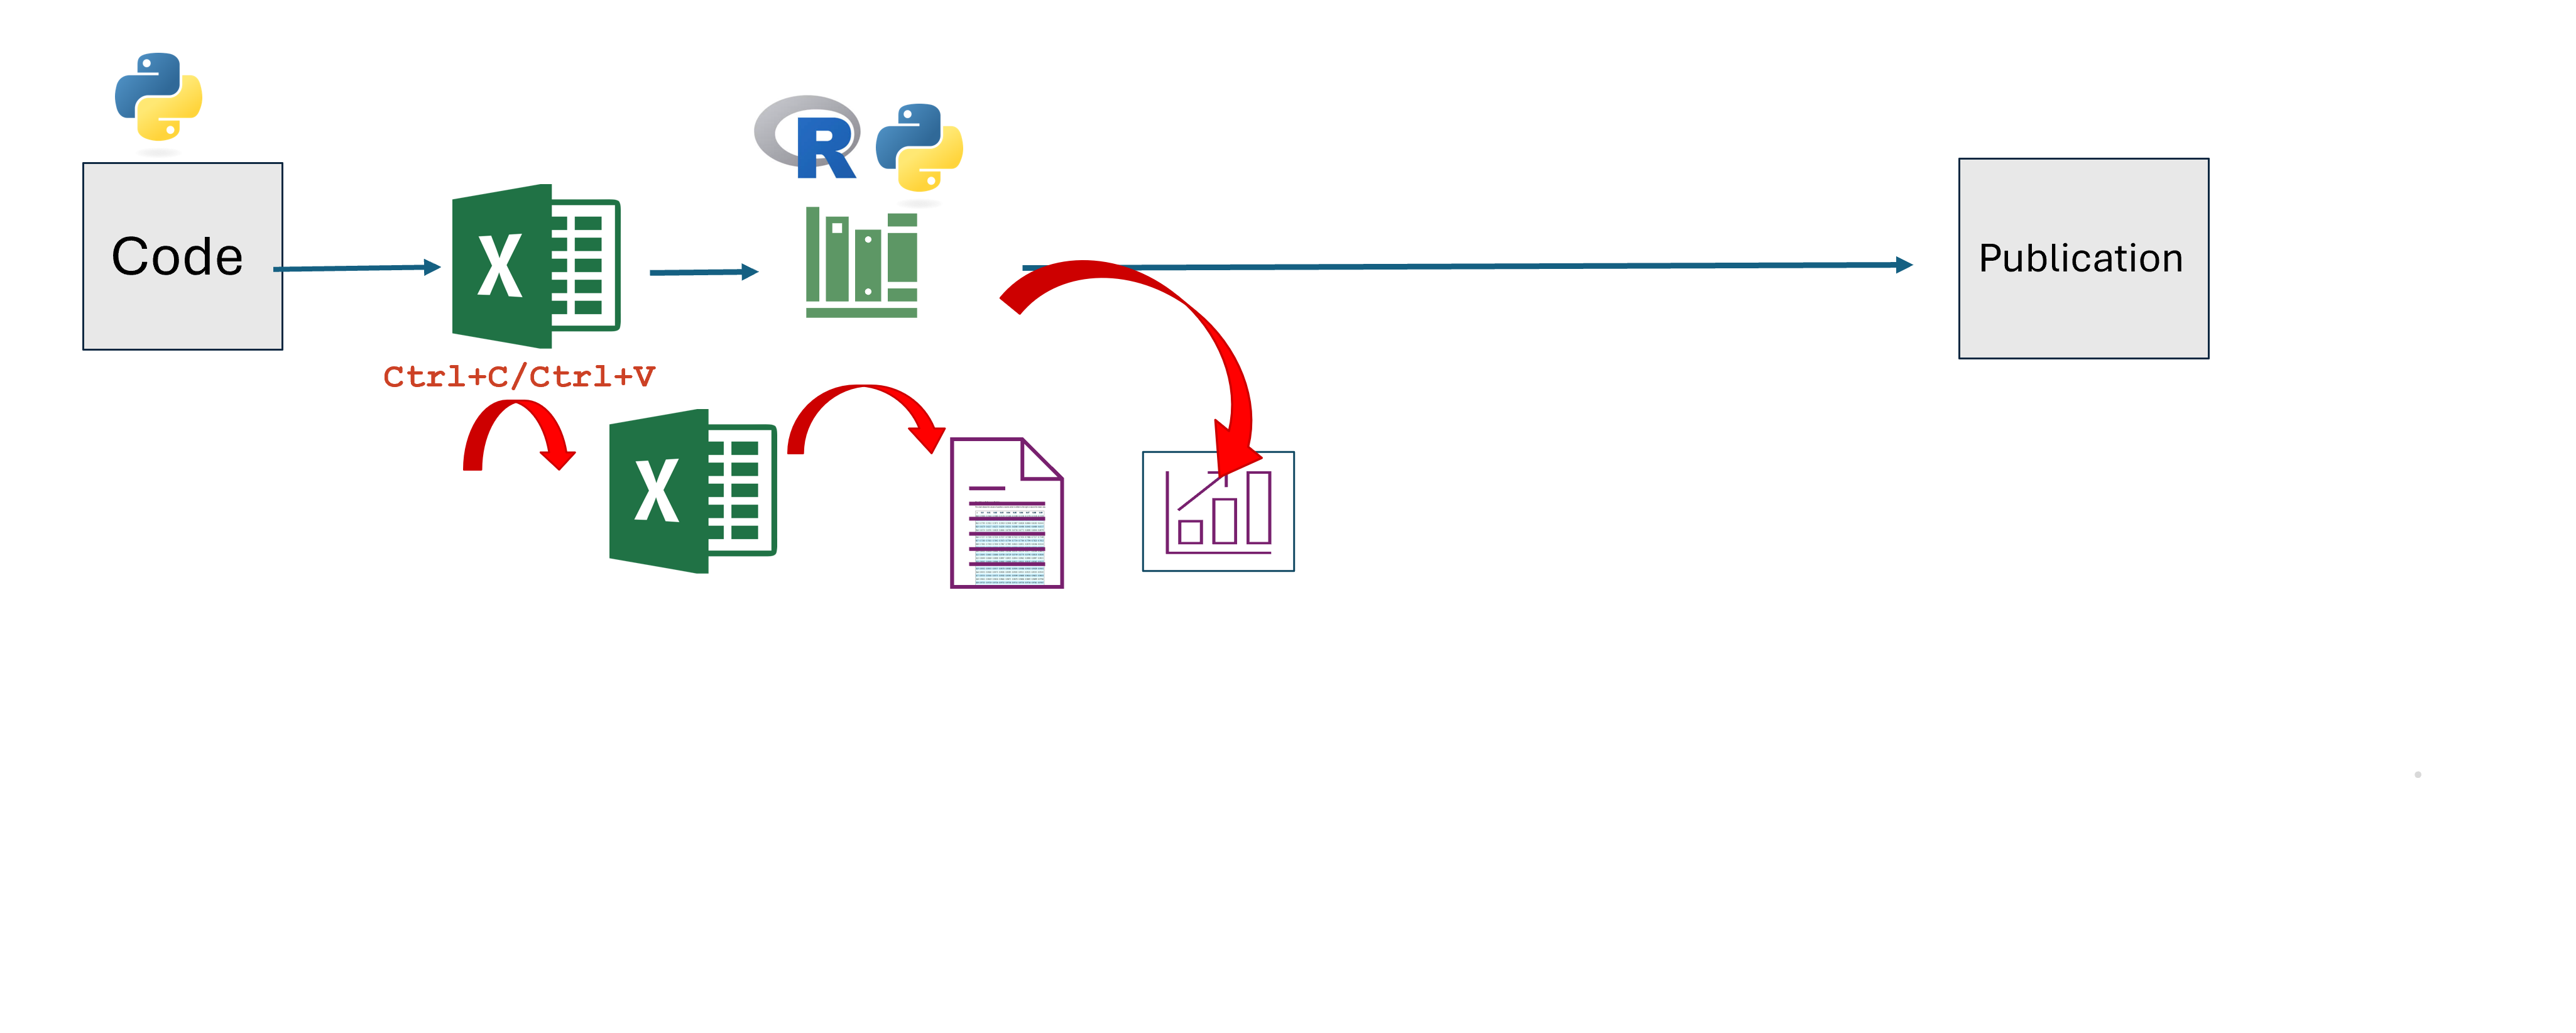
\includegraphics[width=0.8\textwidth]{Process5.png} \\ Comment 5}
        \only<6>{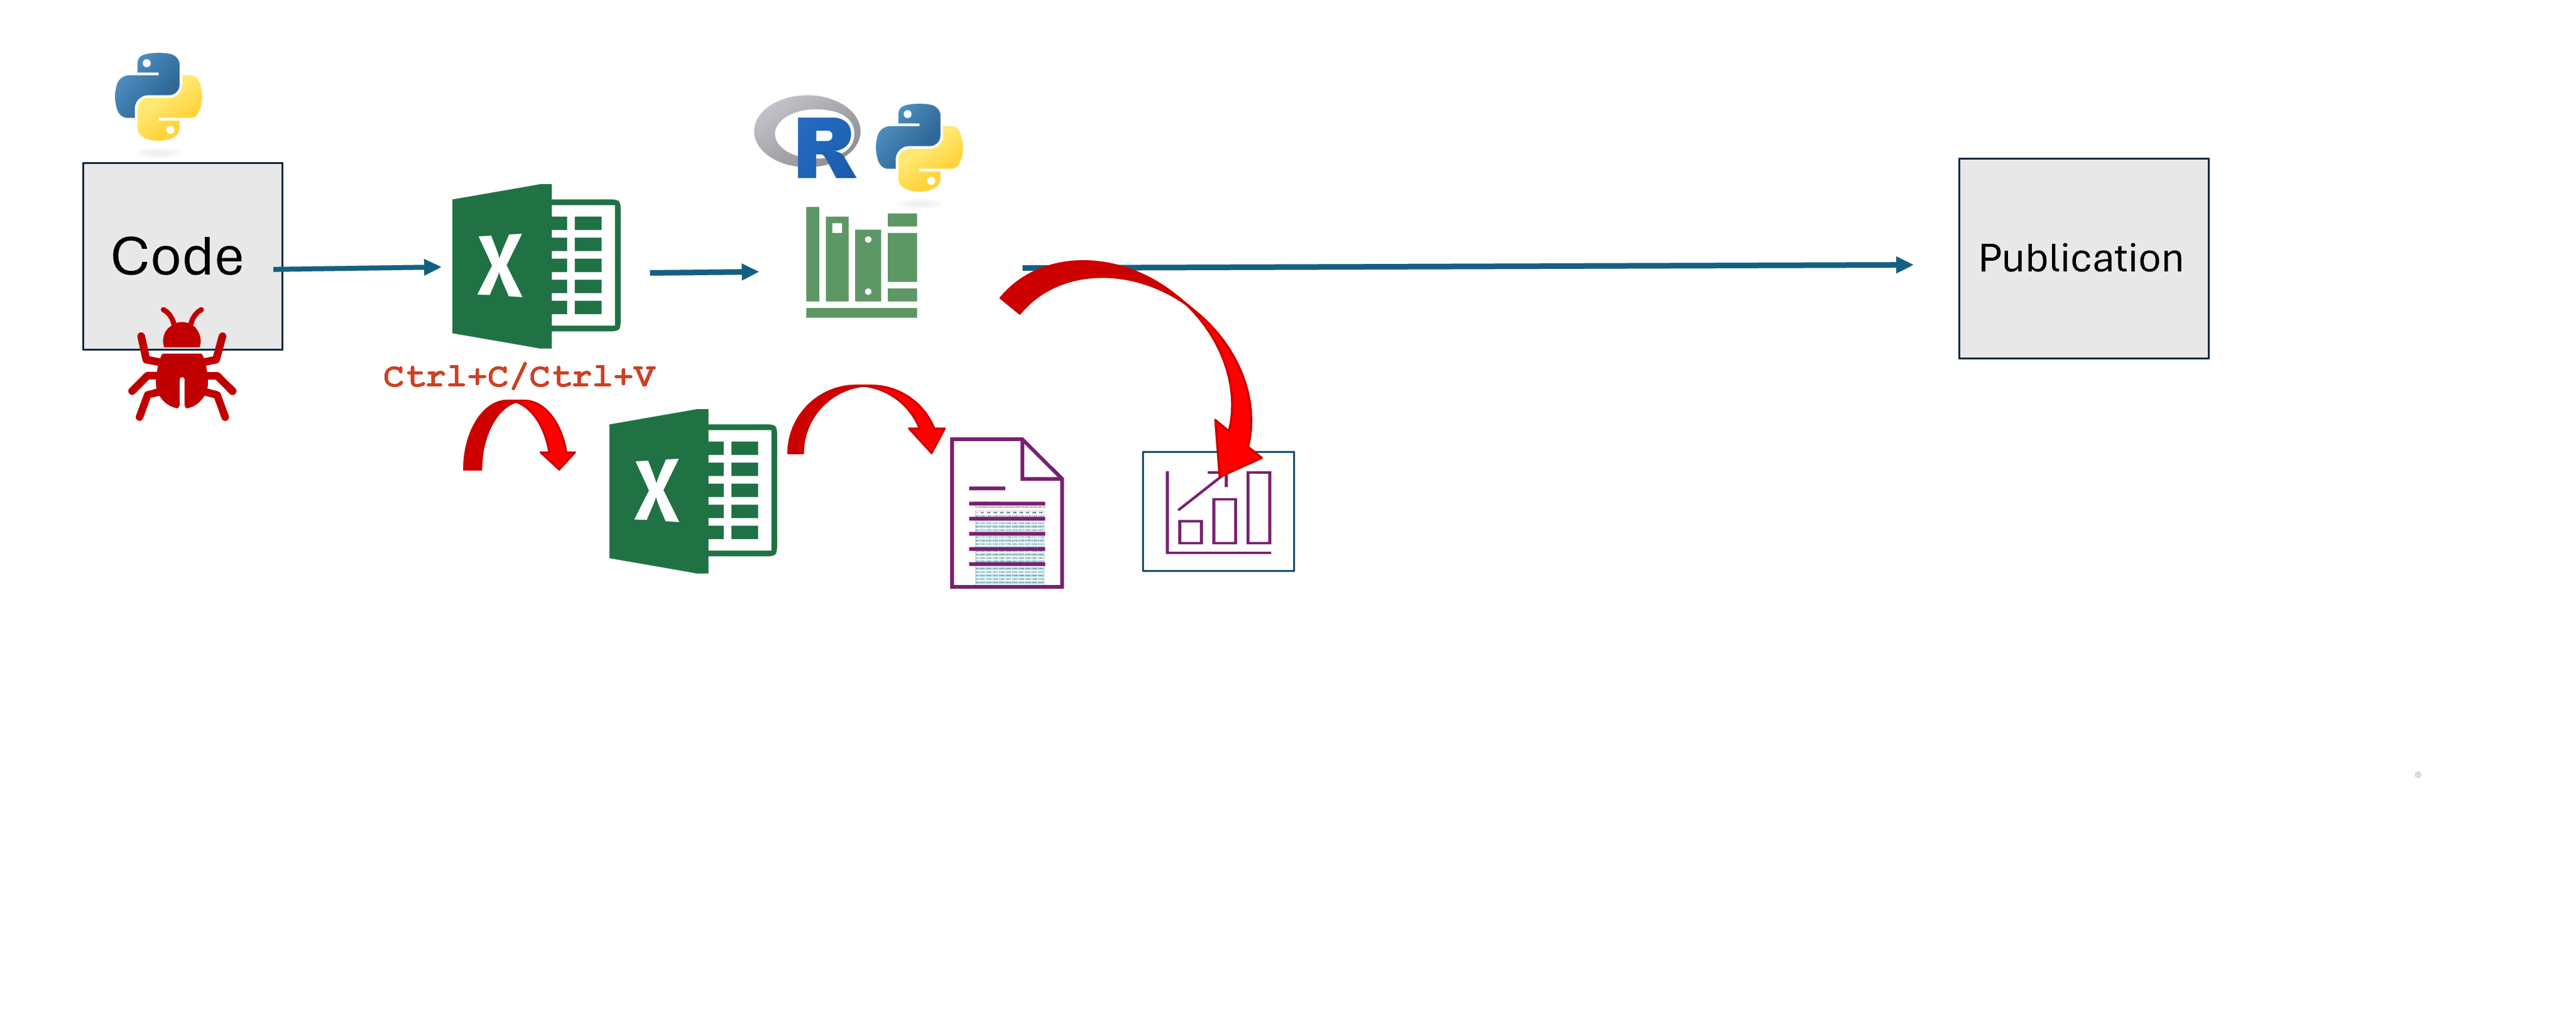
\includegraphics[width=0.8\textwidth]{Process6.png} \\ Comment 6}
        \only<7>{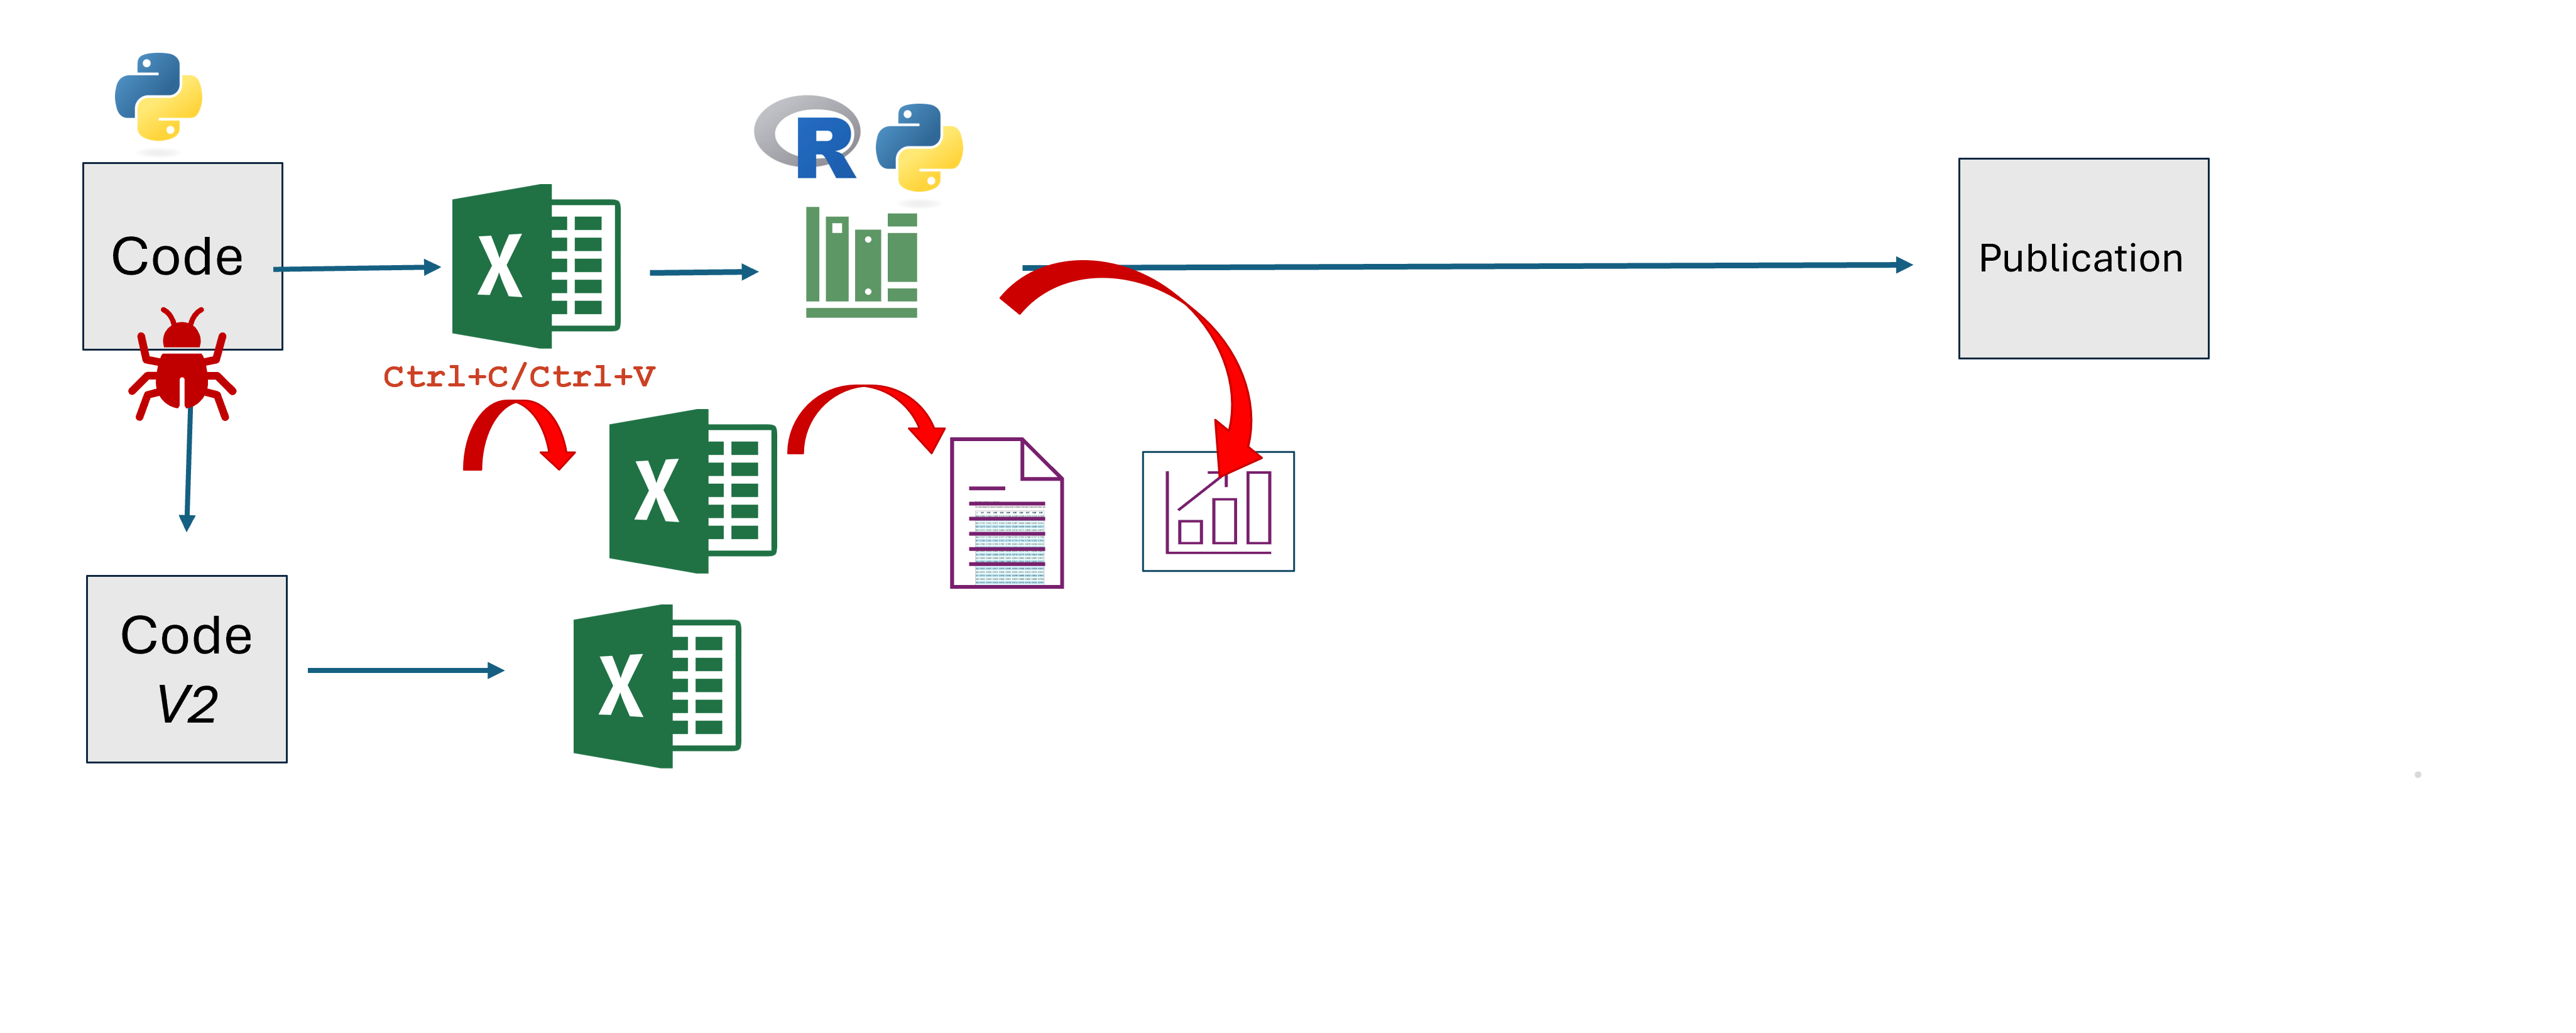
\includegraphics[width=0.8\textwidth]{Process7.png} \\ Comment 7}
        \only<8>{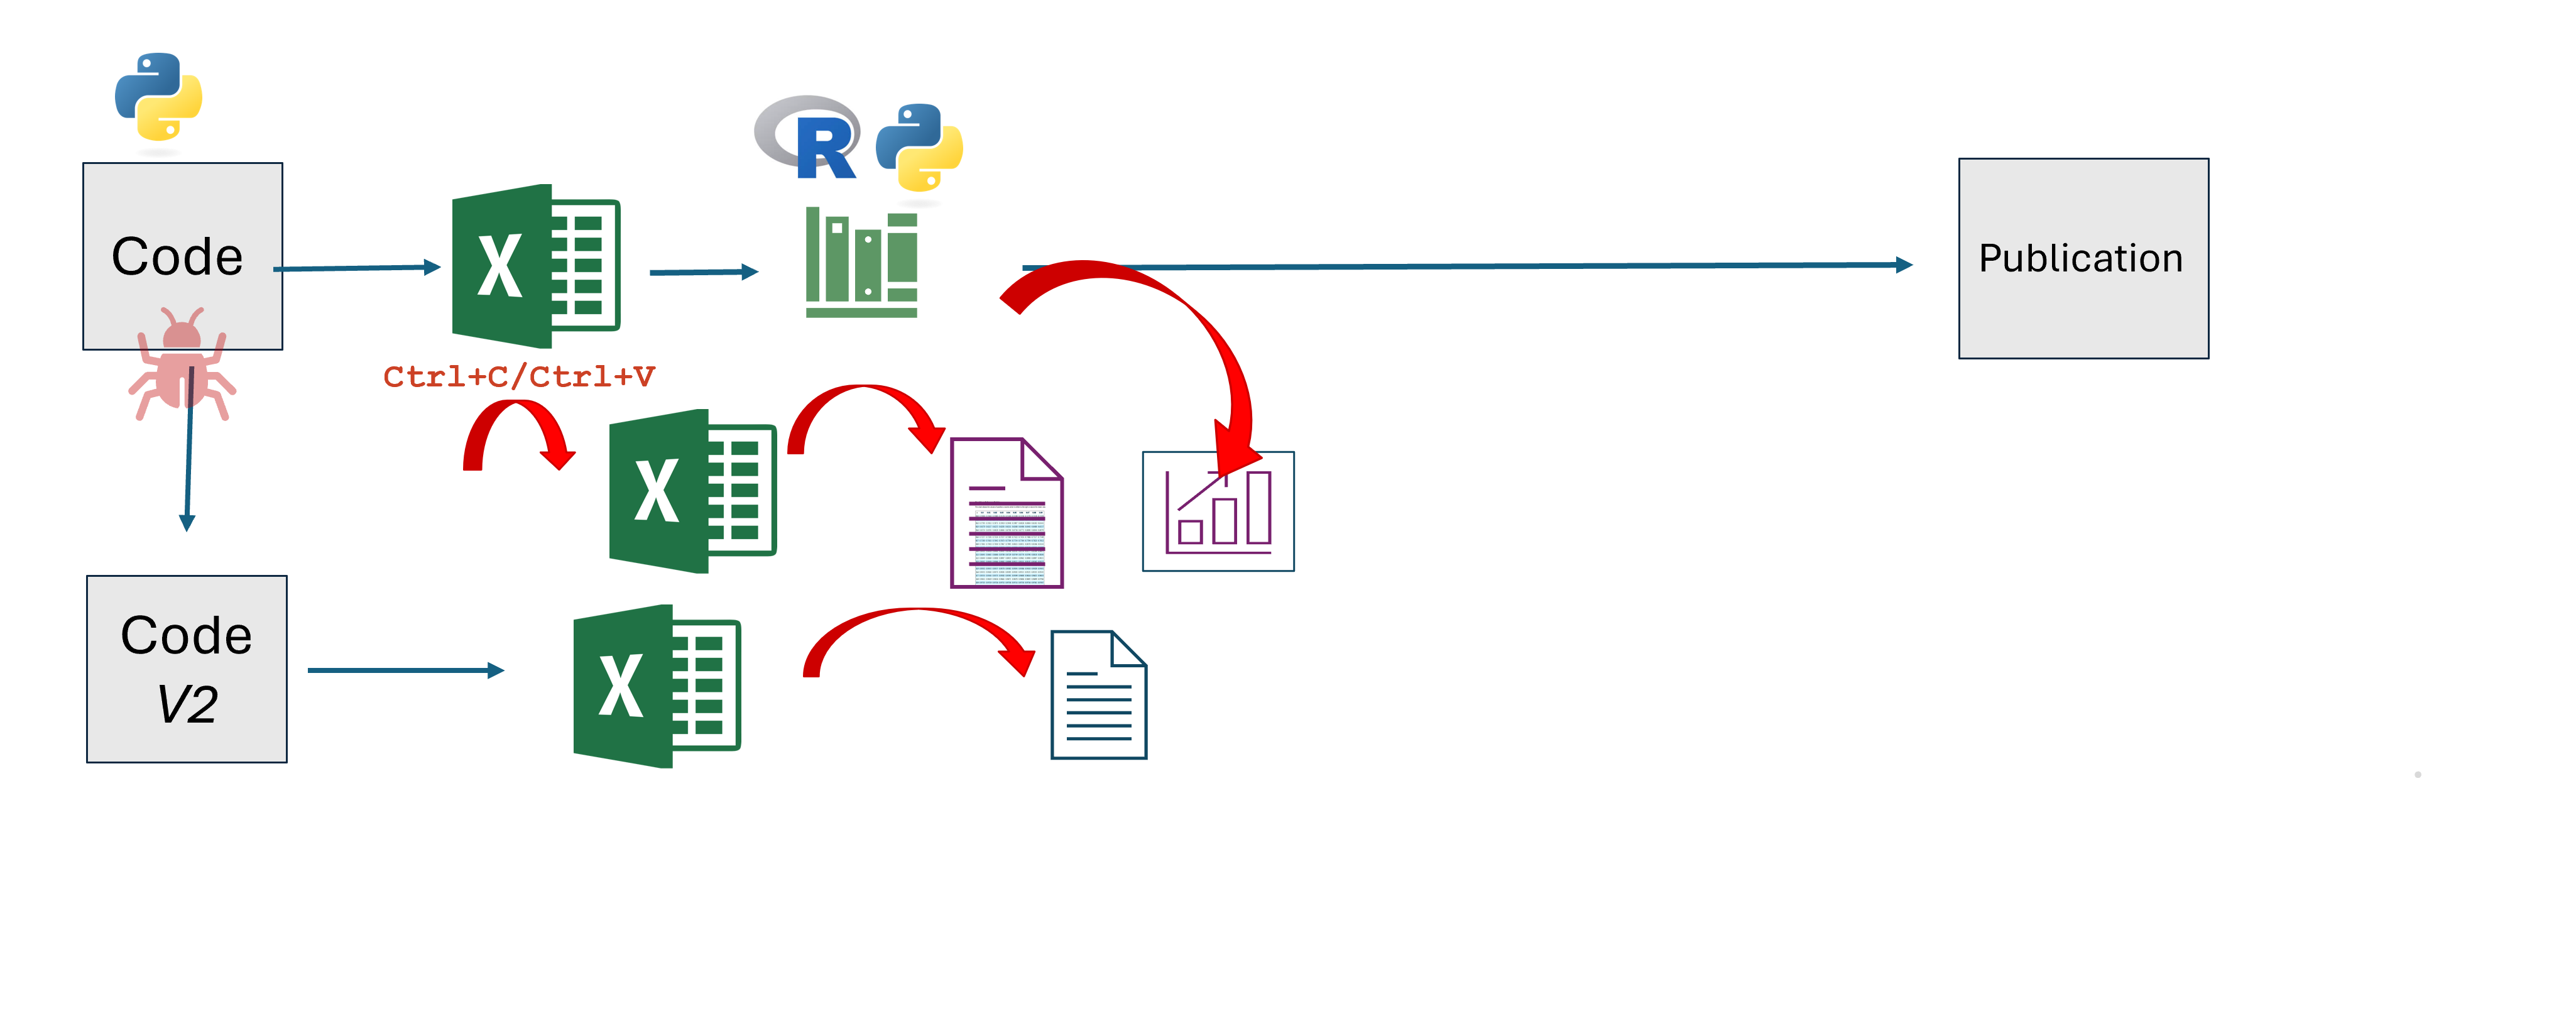
\includegraphics[width=0.8\textwidth]{Process8.png} \\ Comment 8}
        \only<9>{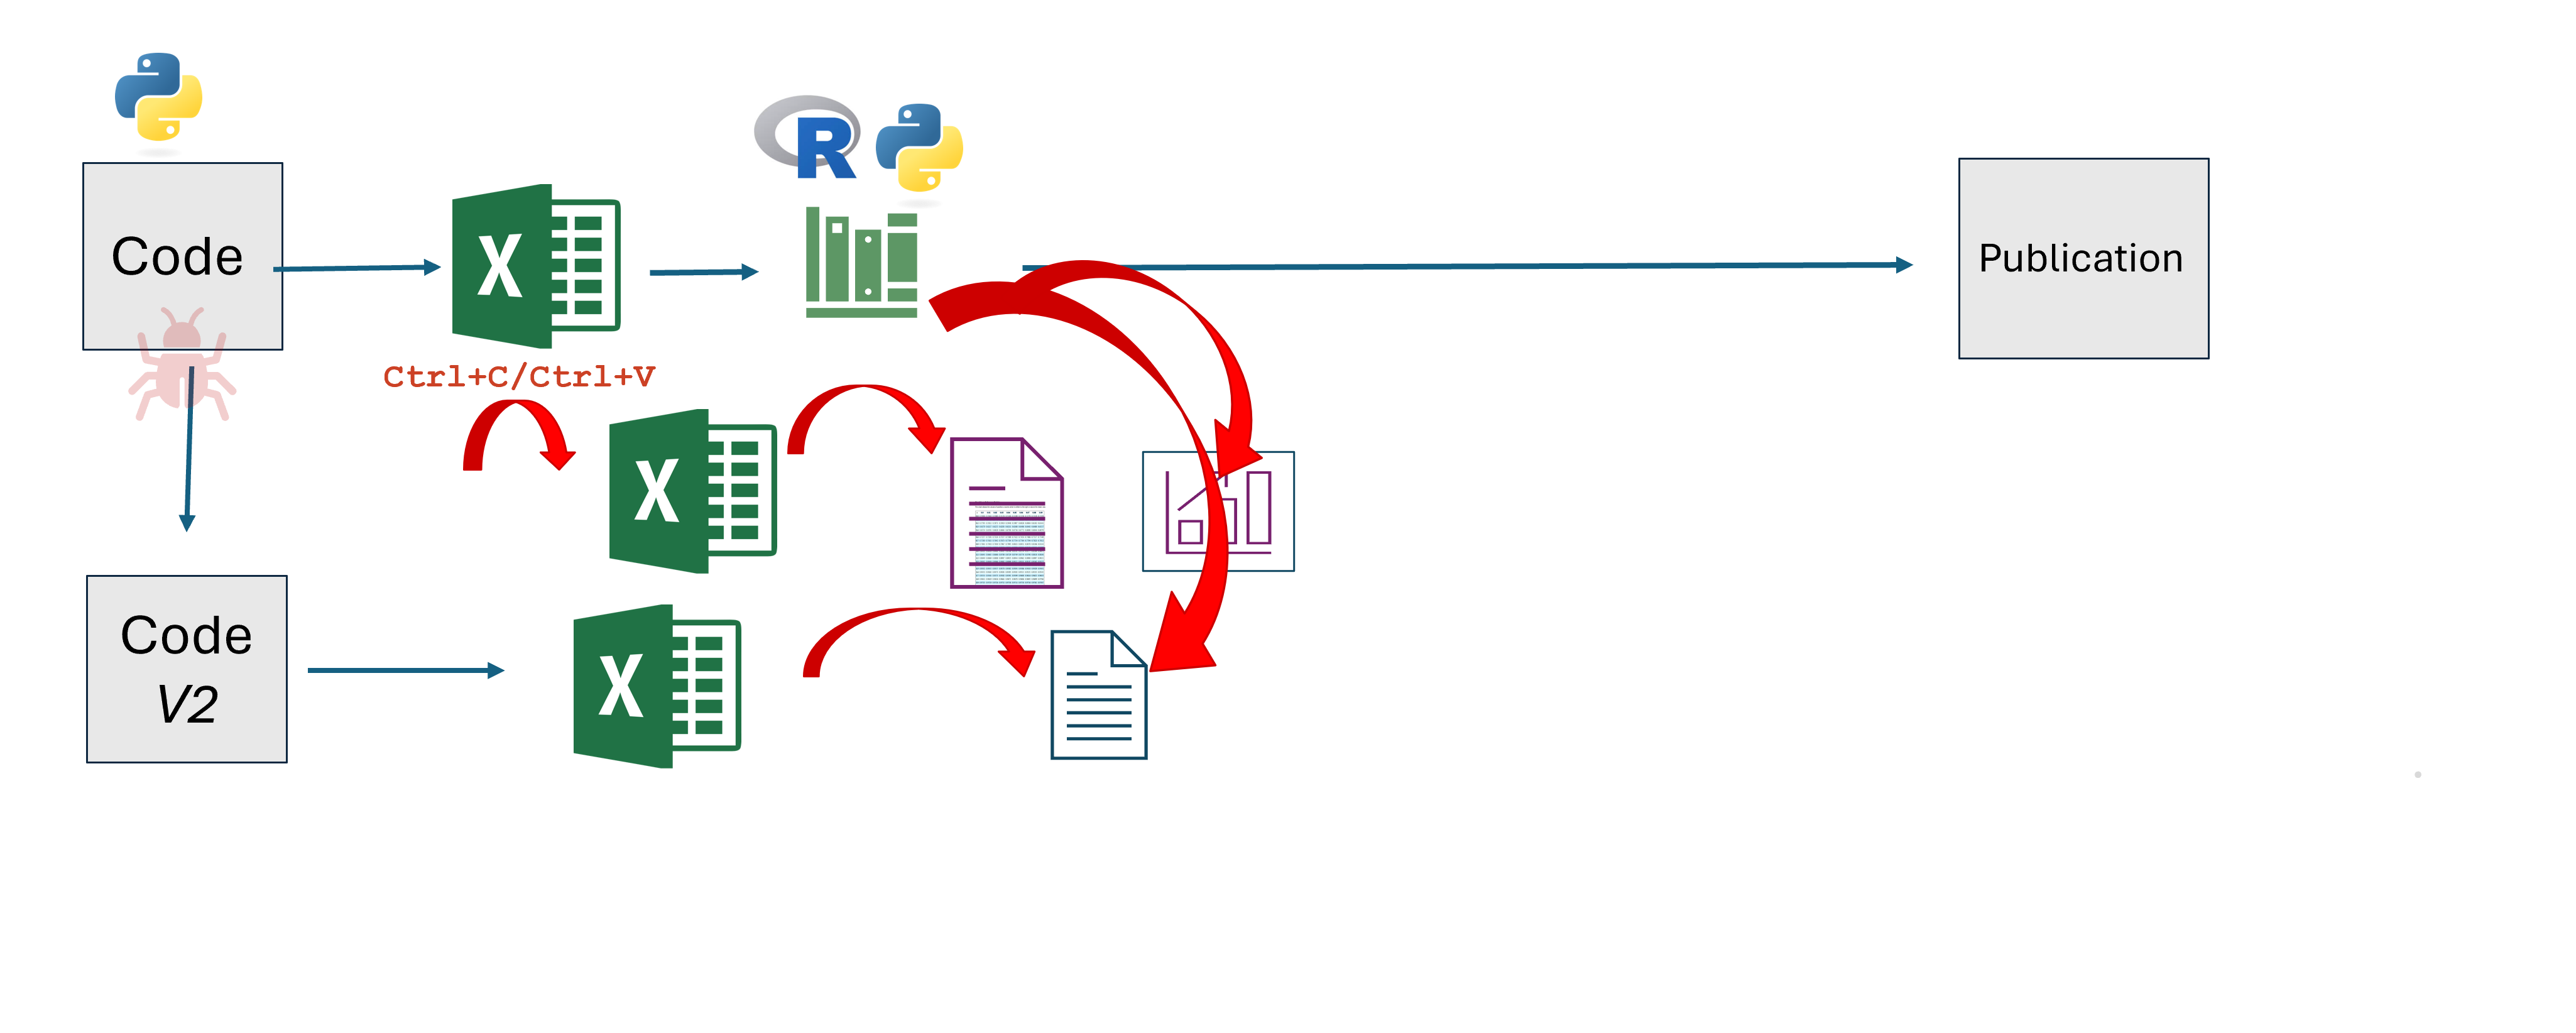
\includegraphics[width=0.8\textwidth]{Process9.png} \\ Comment 9}
        \only<10>{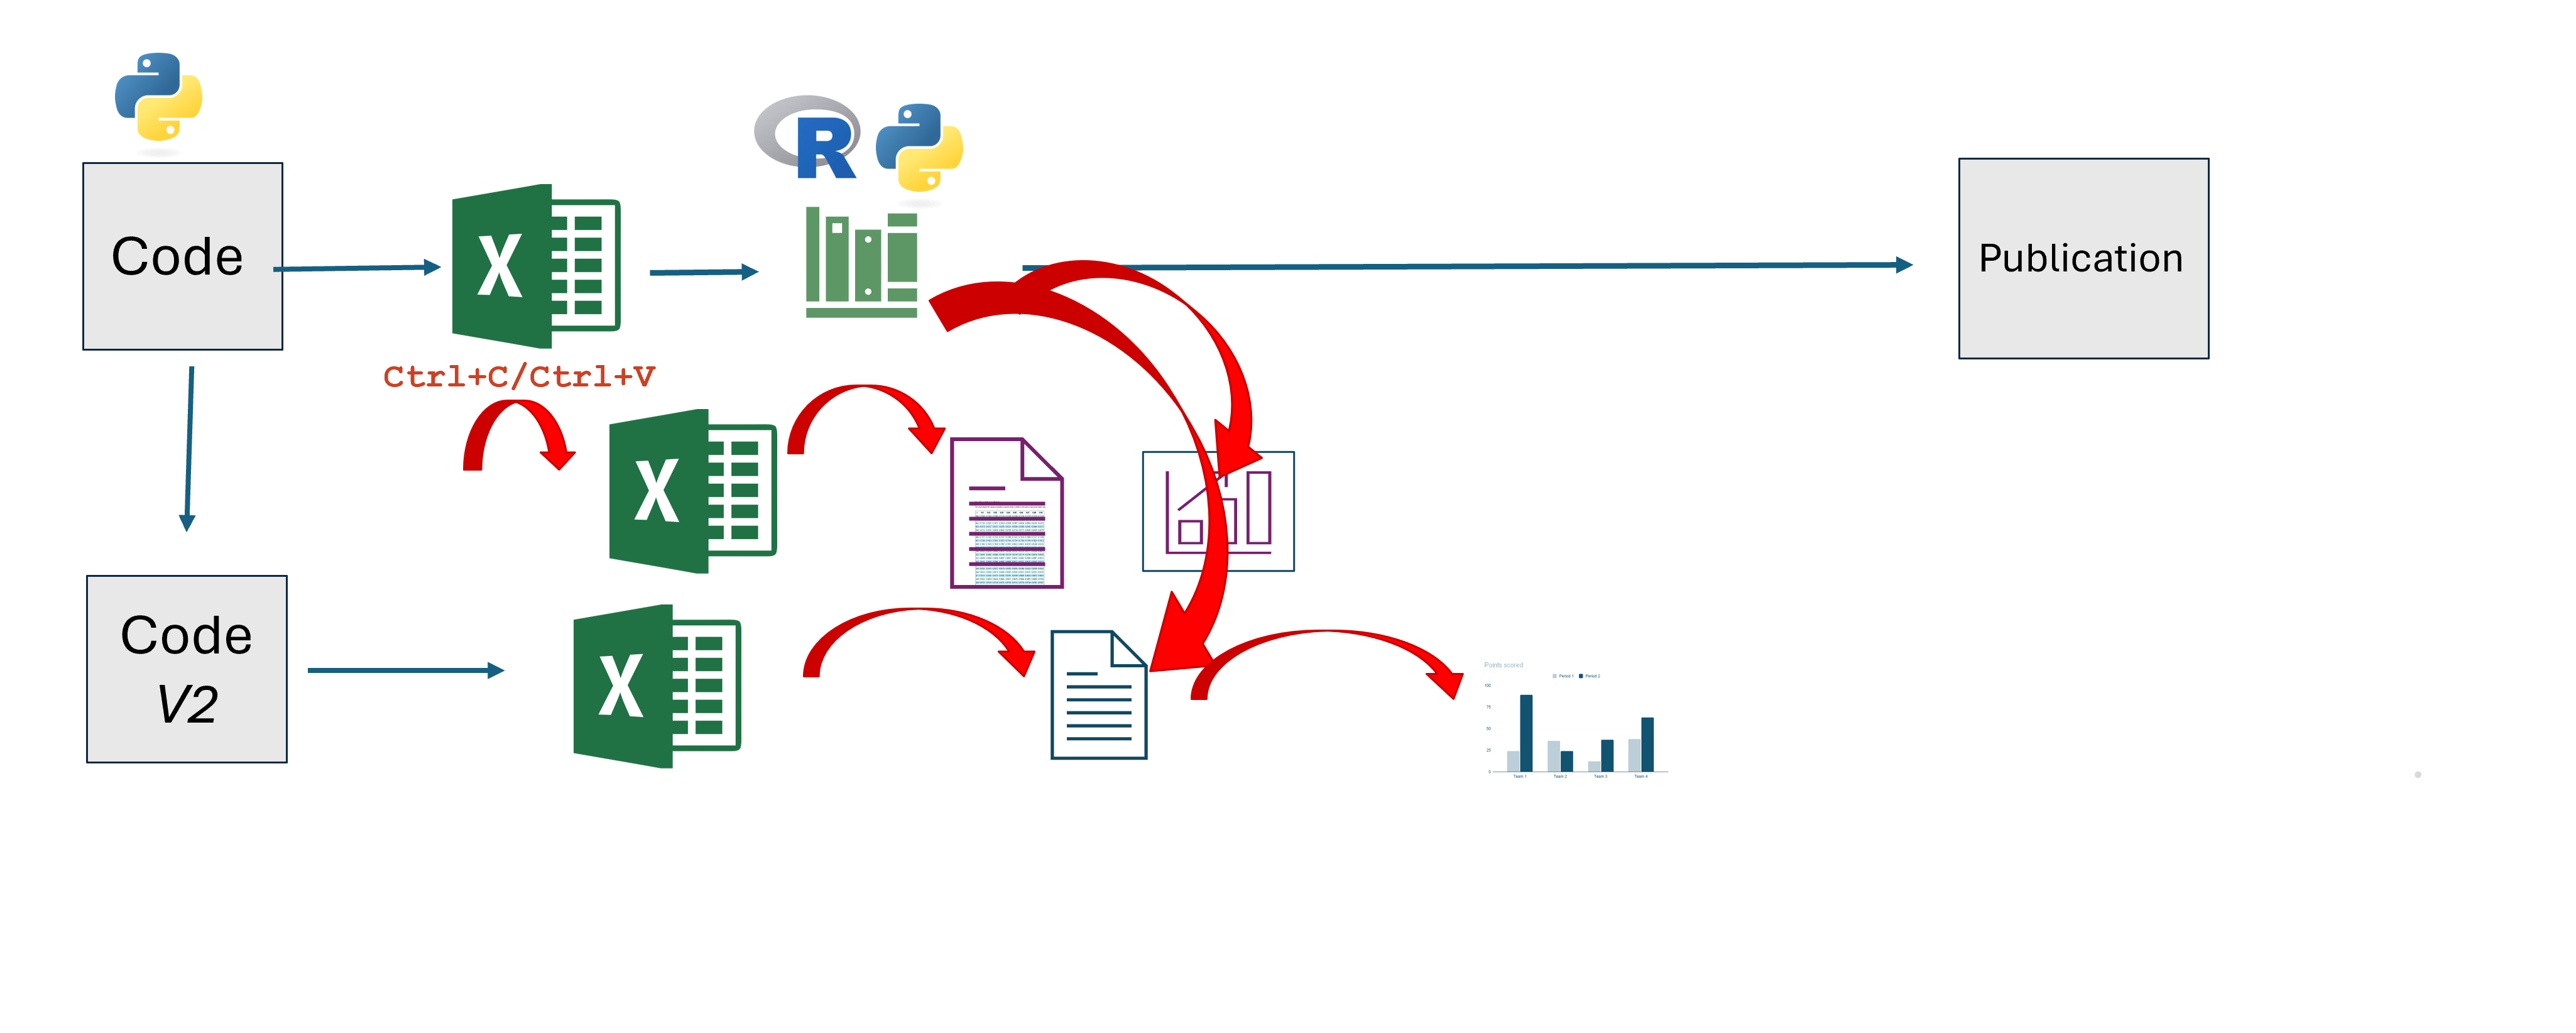
\includegraphics[width=0.8\textwidth]{Process10.png} \\ Comment 10}
        \only<11>{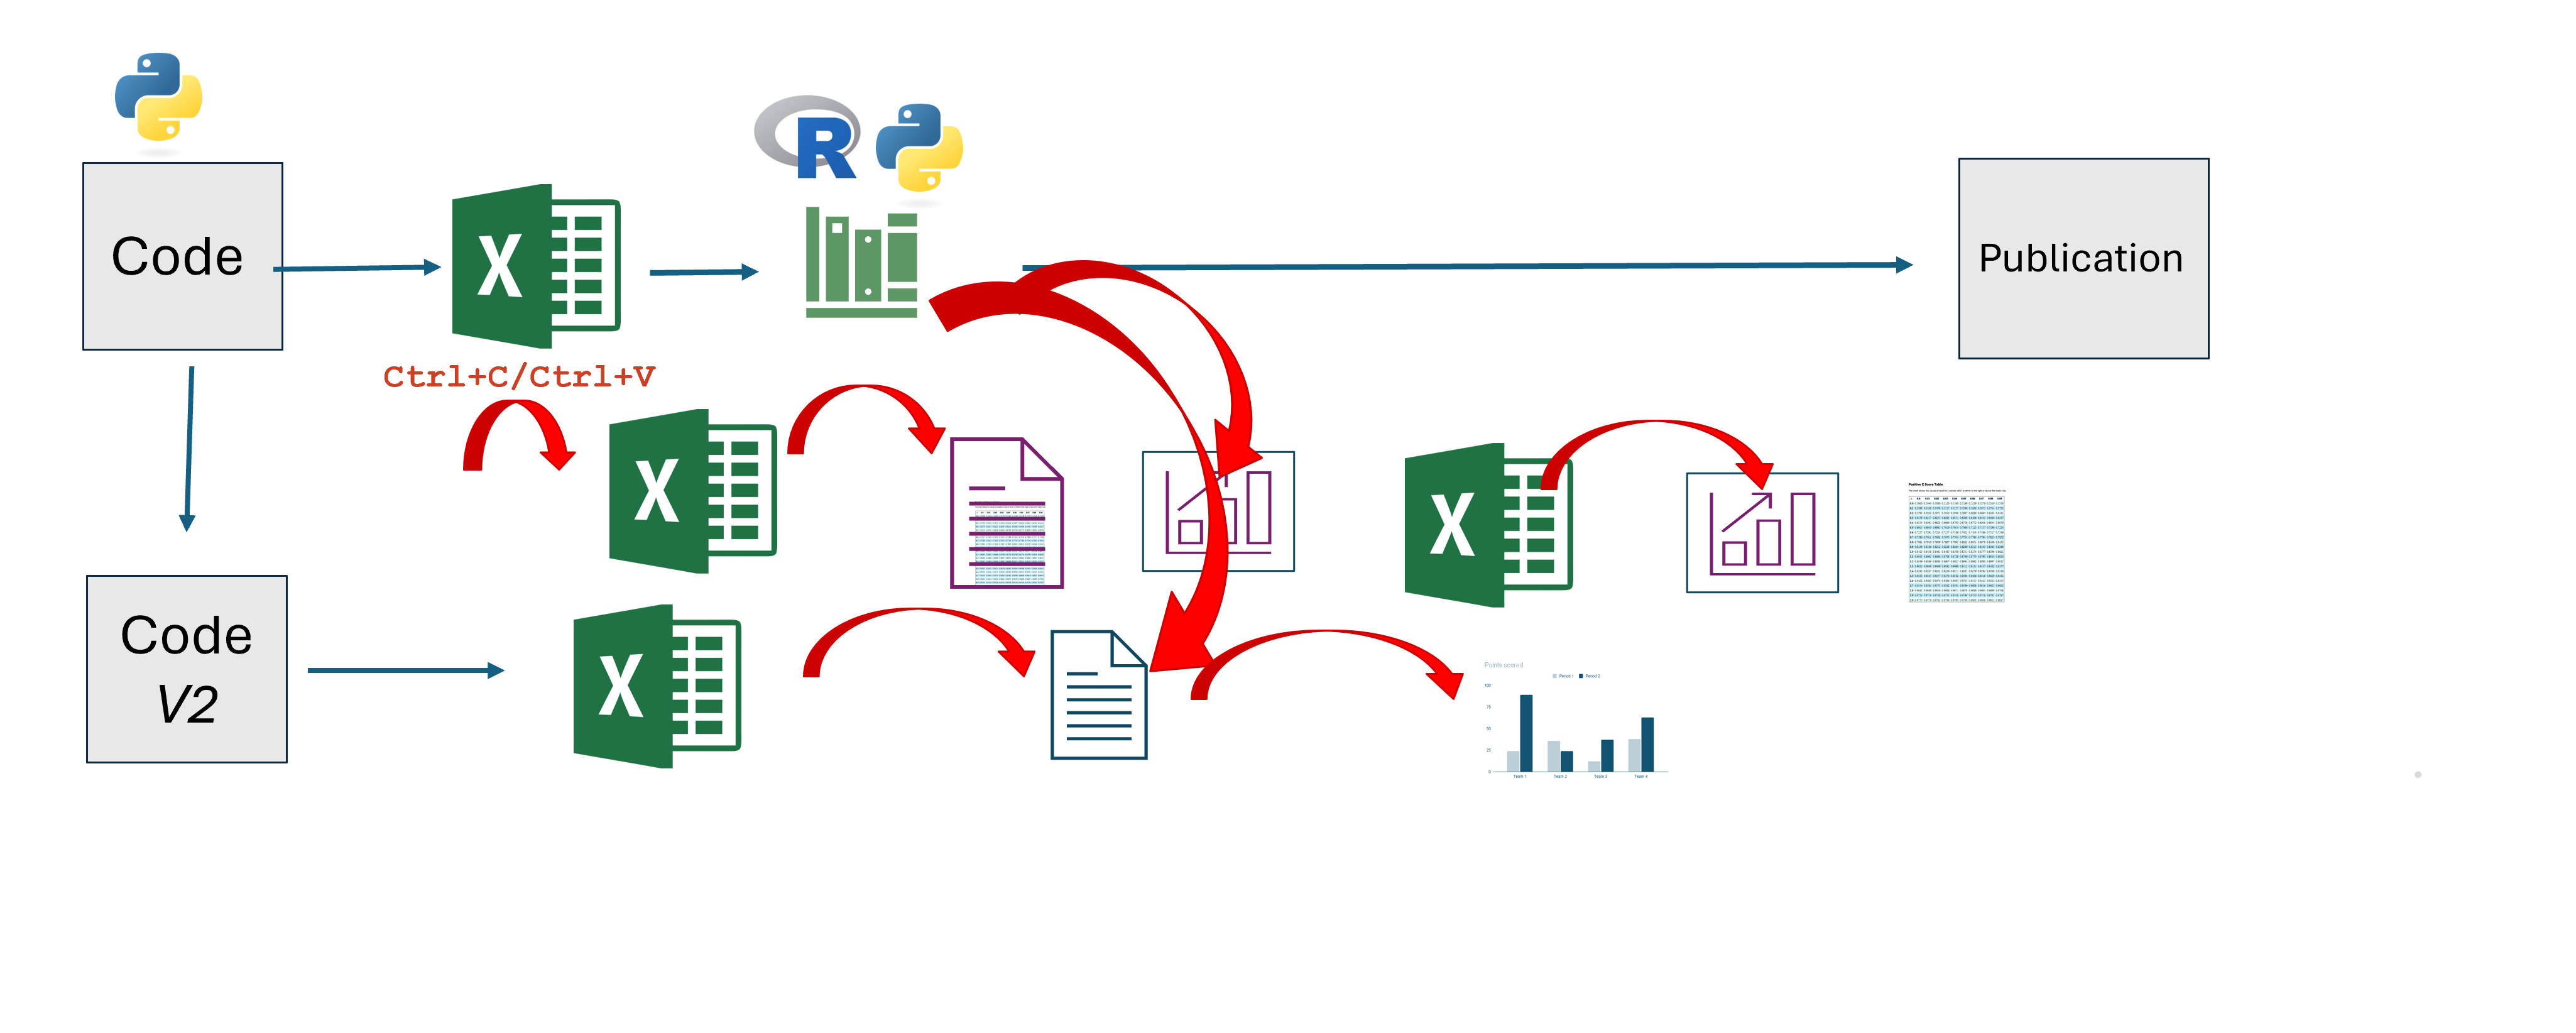
\includegraphics[width=0.8\textwidth]{Process11.png} \\ Comment 9}
        \only<12>{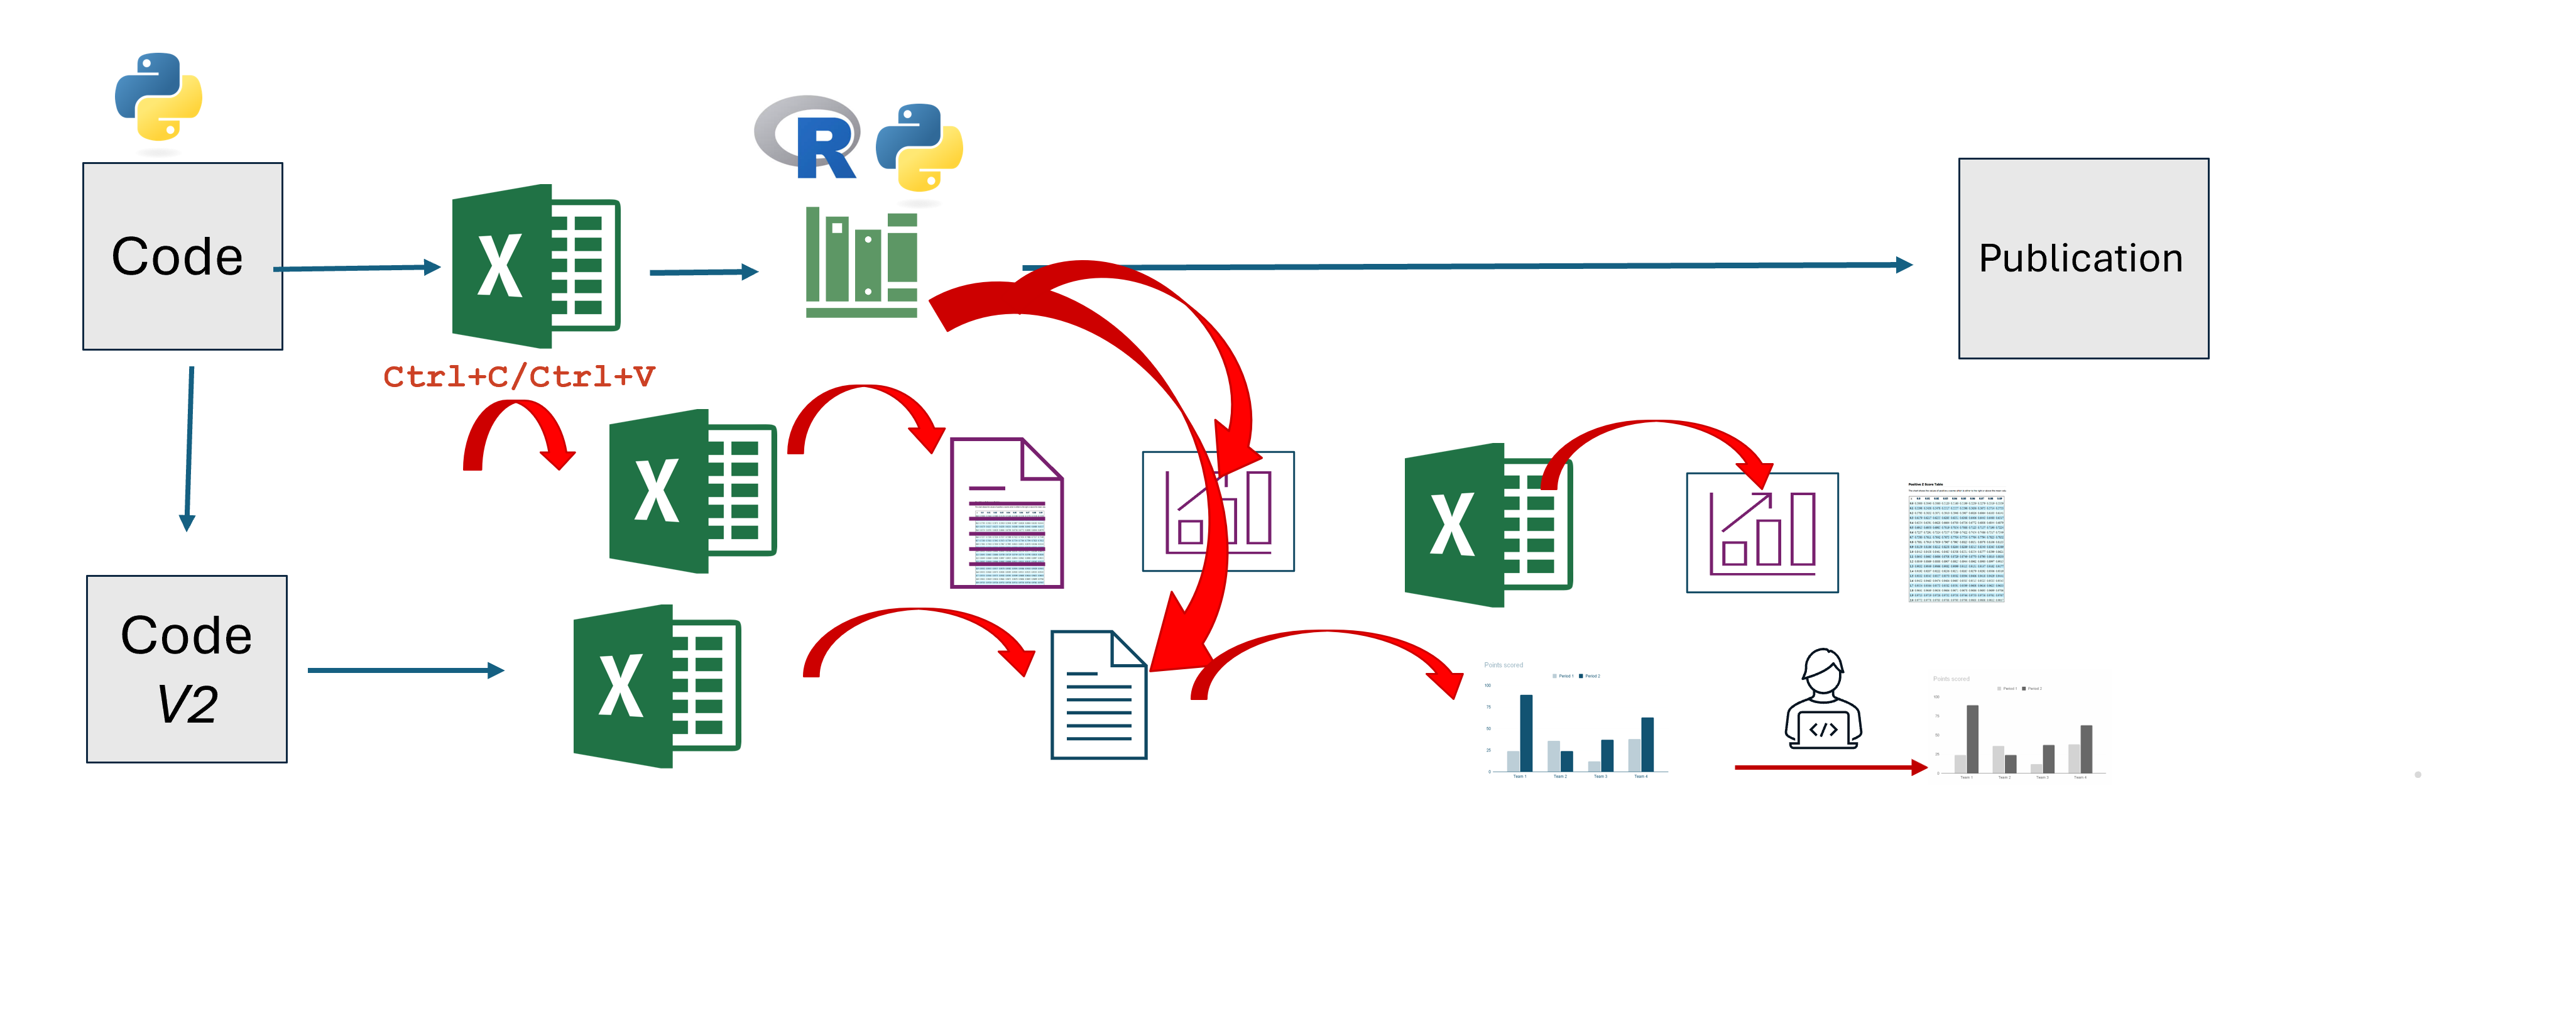
\includegraphics[width=0.8\textwidth]{Process12.png} \\ Comment 10}
        \only<13>{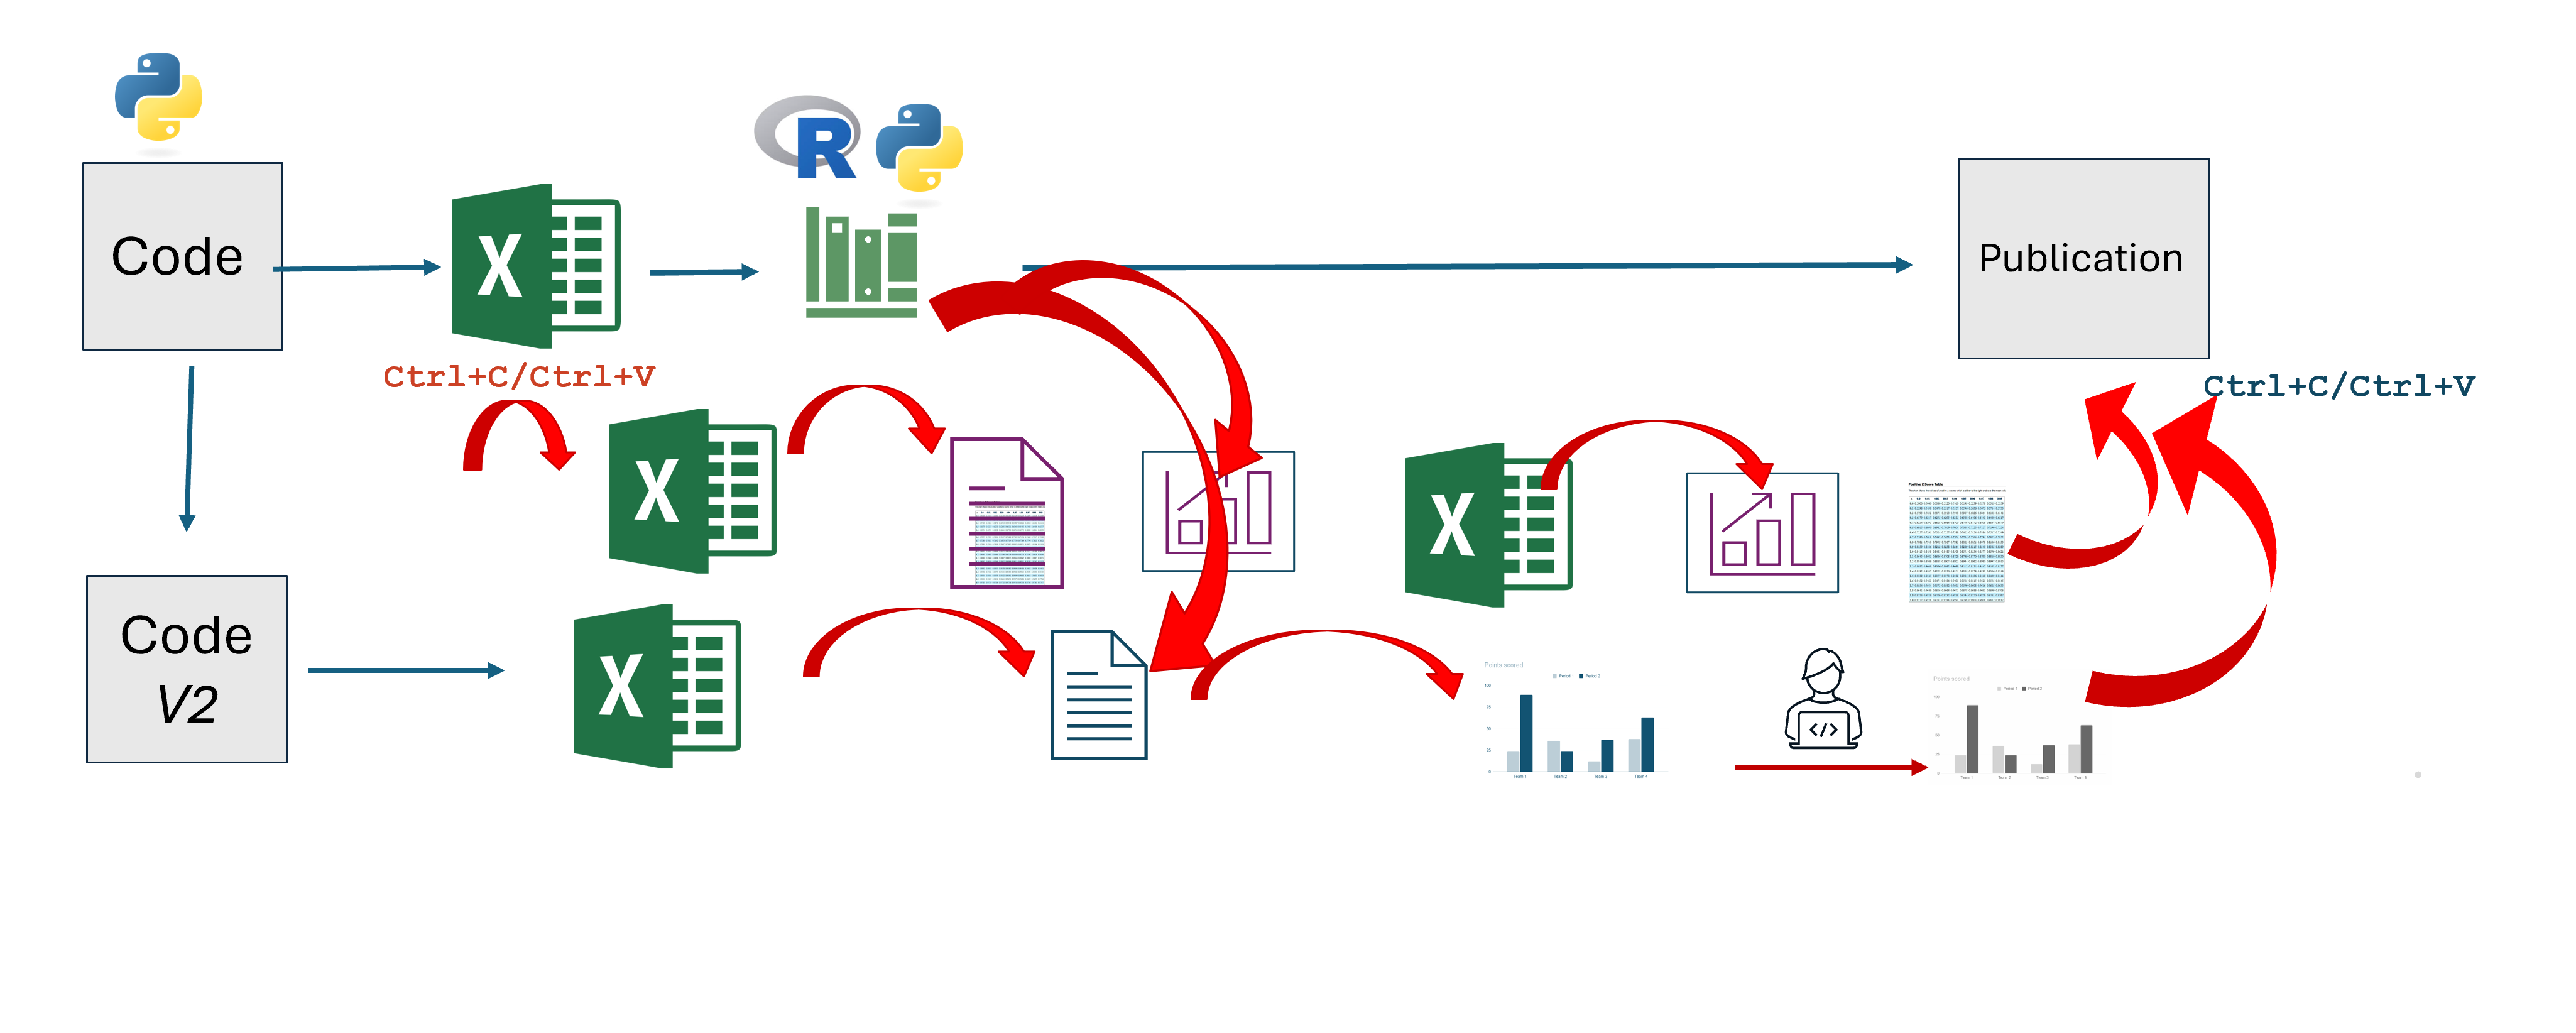
\includegraphics[width=0.8\textwidth]{Process13.png} \\ Comment 9}
        \only<14>{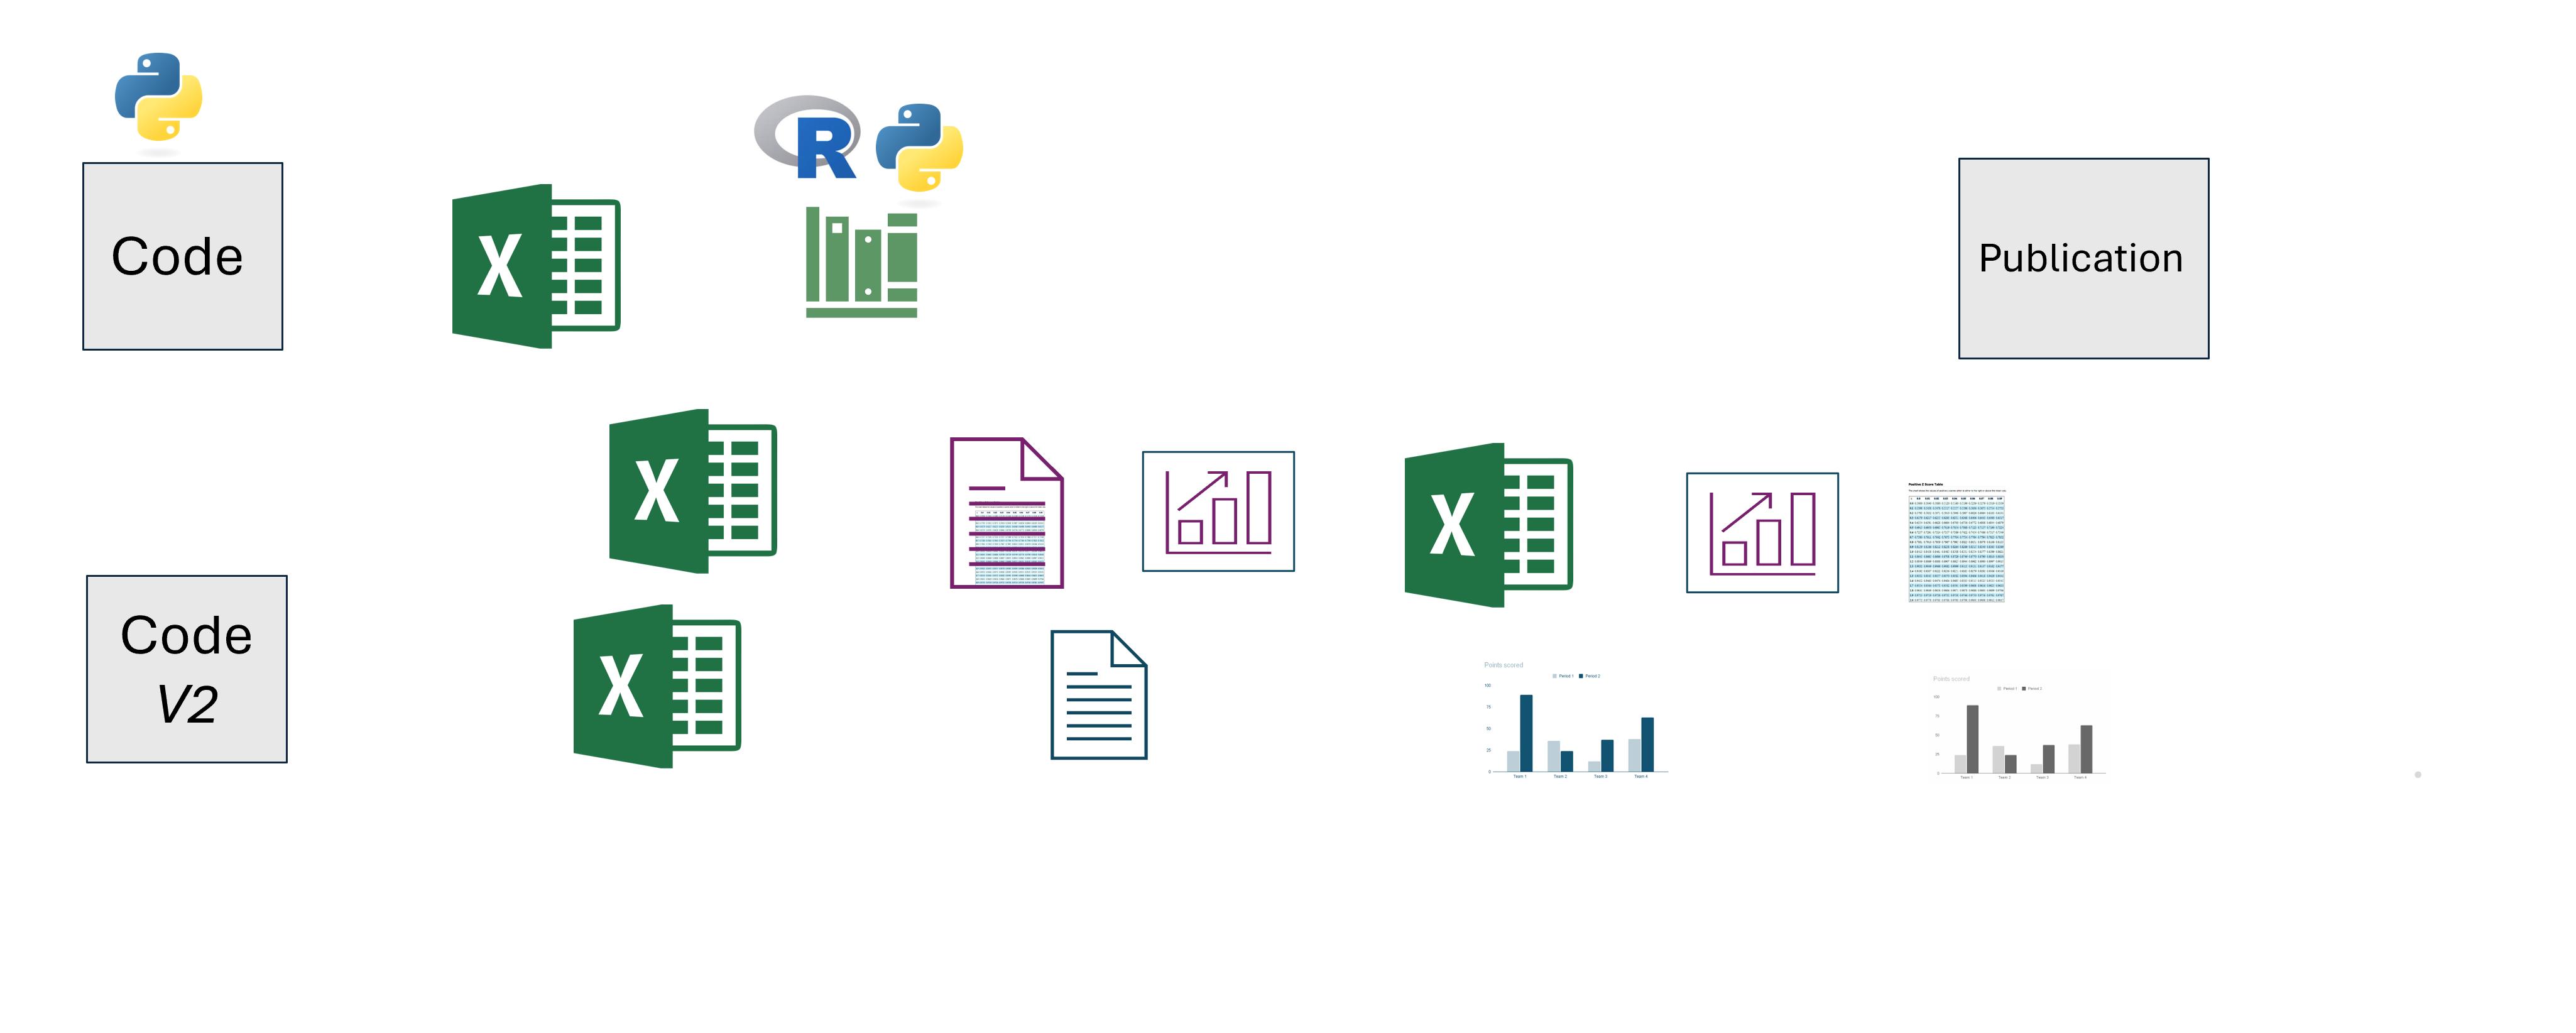
\includegraphics[width=0.8\textwidth]{Process14.png} \\ Comment 10}
    \end{itemize}
\end{center}
\end{frame}


\begin{frame}{Usual practice: In the end}

 \begin{columns}[T]
    \begin{column}{0.5\textwidth}
      \begin{itemize}[<+->]
        \item Lots of files
        \item Cut and paste is not a reliable, reproducible approach!
        \item Your brain may remember..
        \item[] ...all the steps...
        \item[] .. in the right order..
        \item[]...all of them !
        \item Or use (bad) "\emph{tools}"
      \end{itemize}
    \end{column}
    \begin{column}{0.5\textwidth}
       \begin{itemize}
       \item[] \only<1>{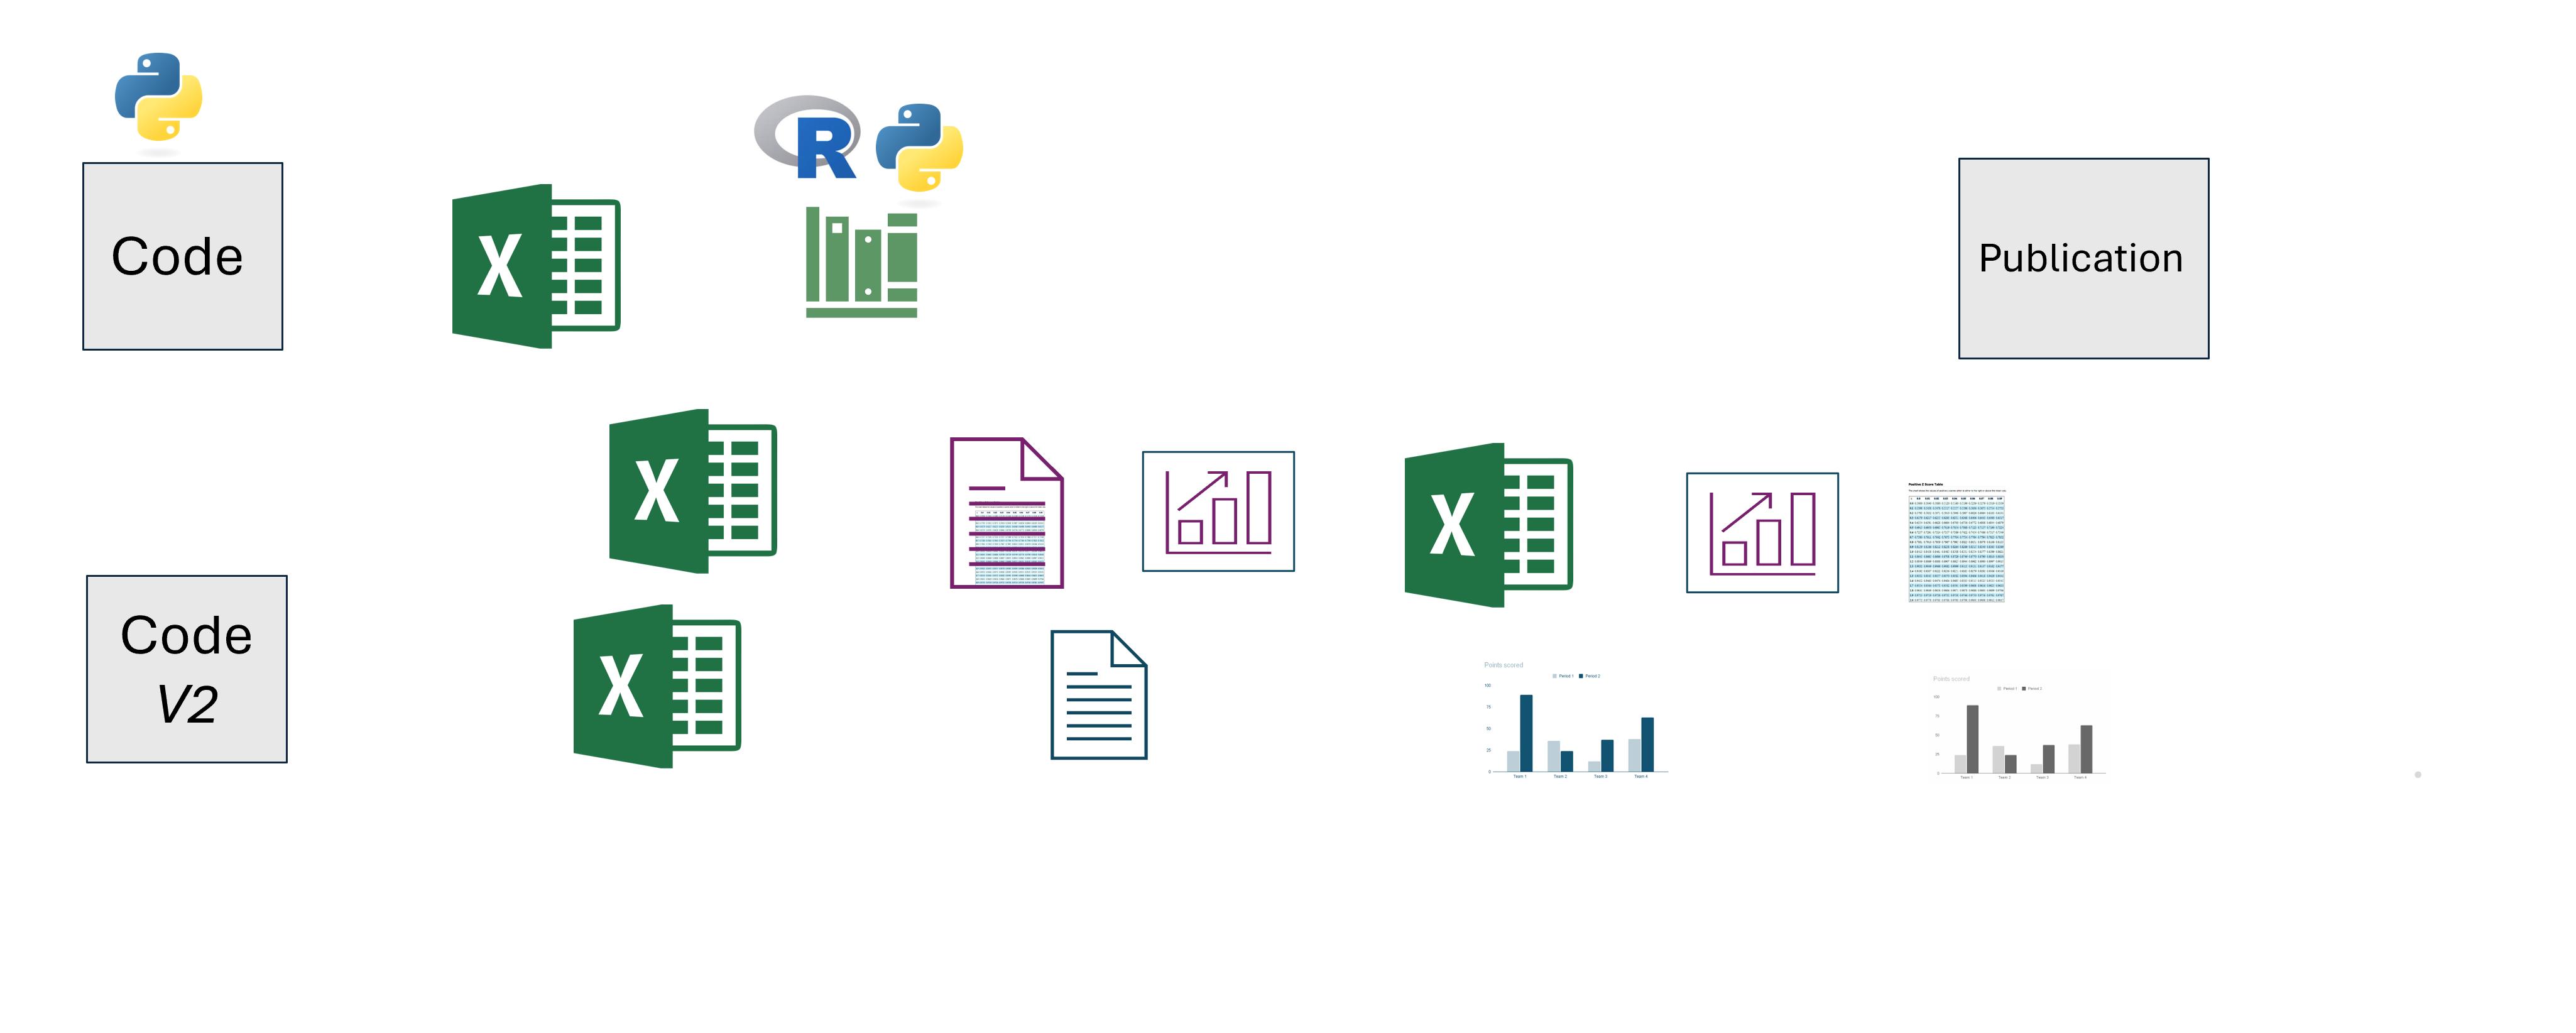
\includegraphics[width=0.8\textwidth]{Process14.png} }
        \only<2>{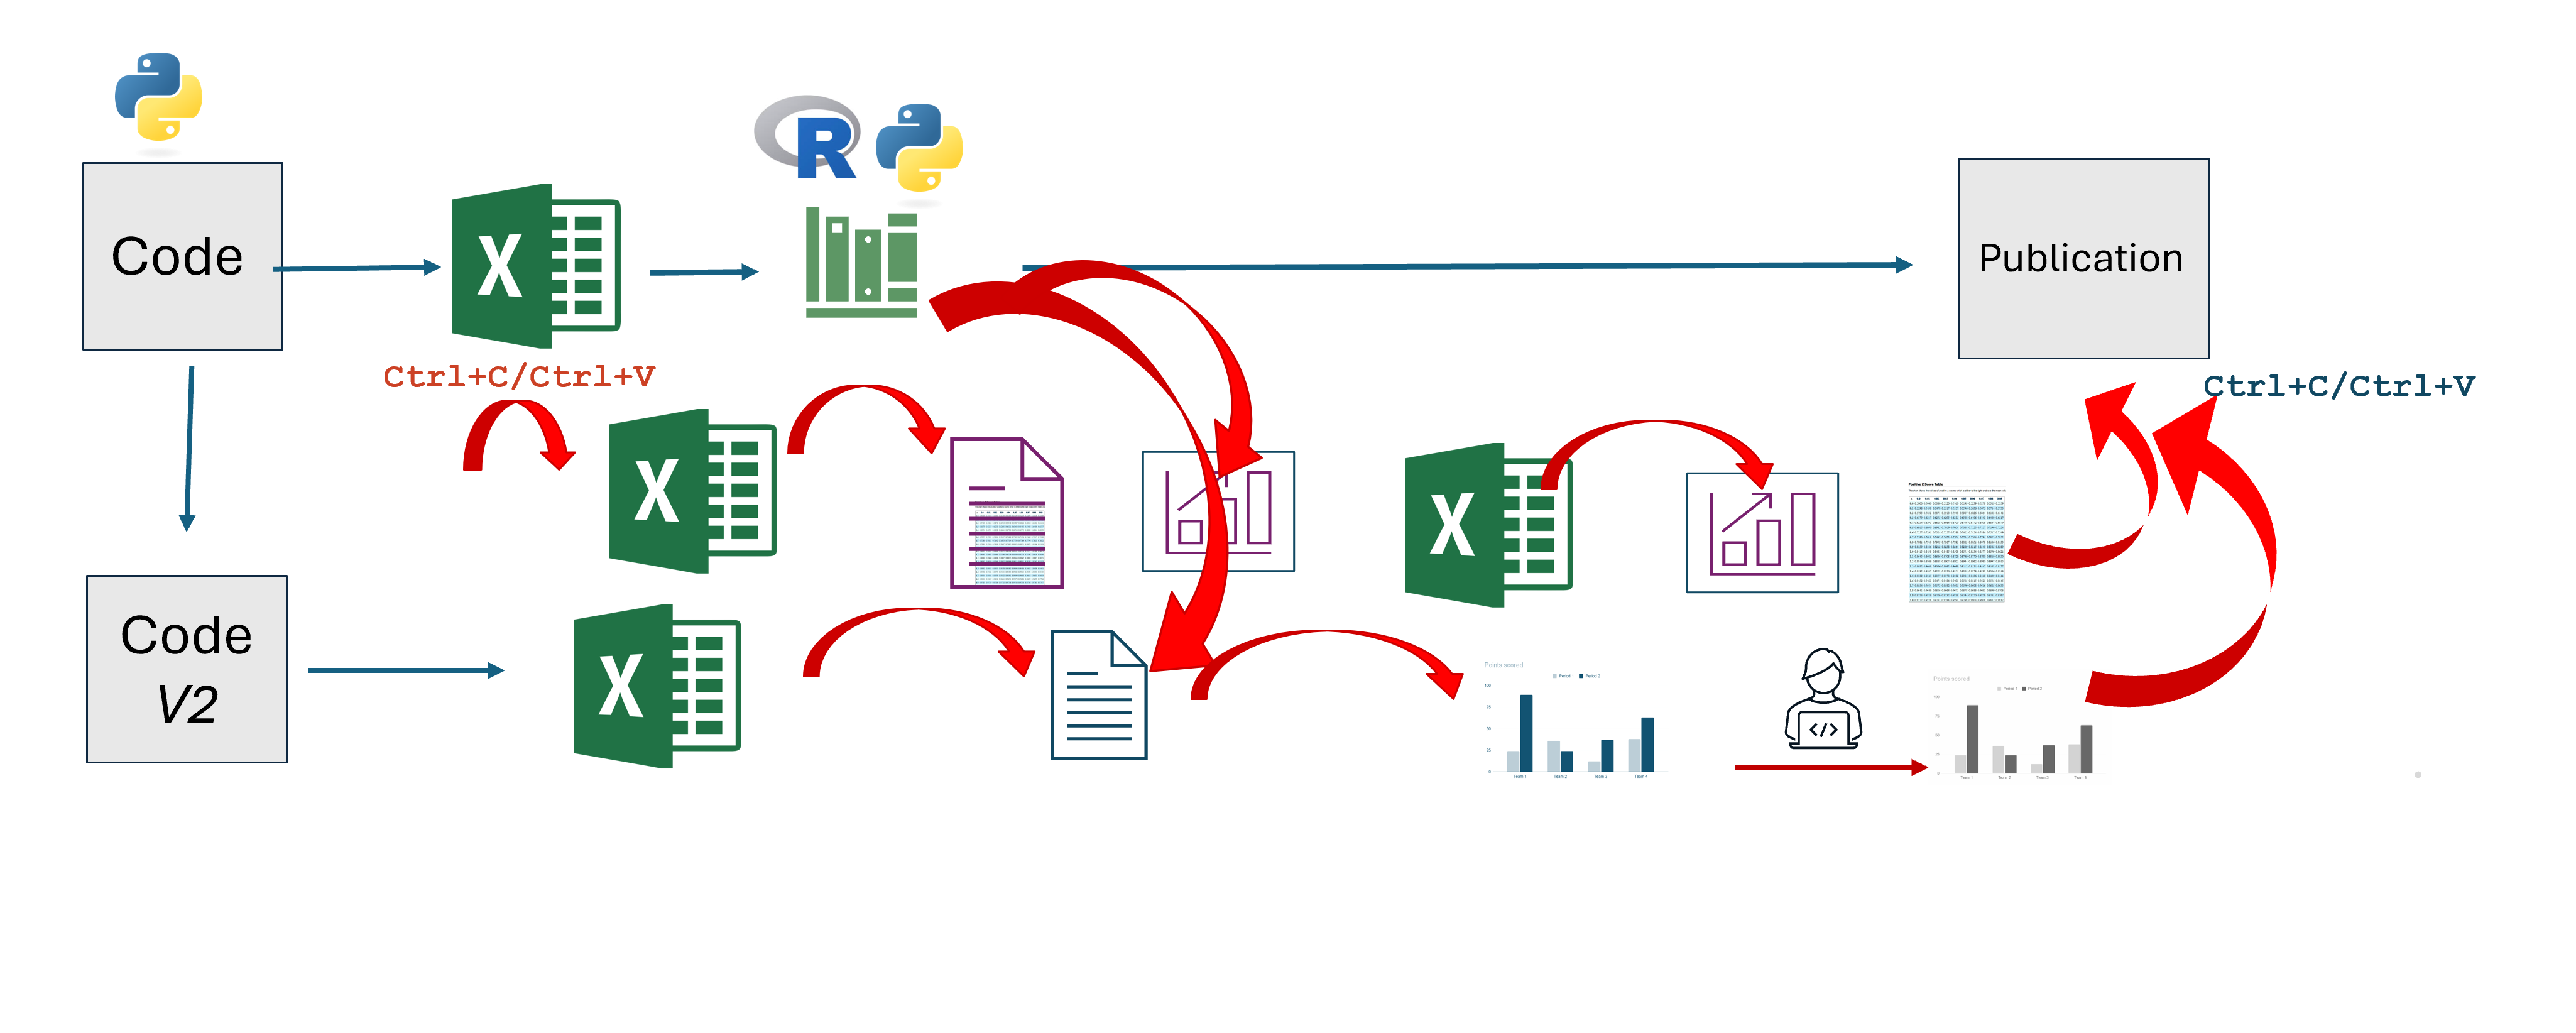
\includegraphics[width=1.0\textwidth]{Process13.png} }
        \only<3>{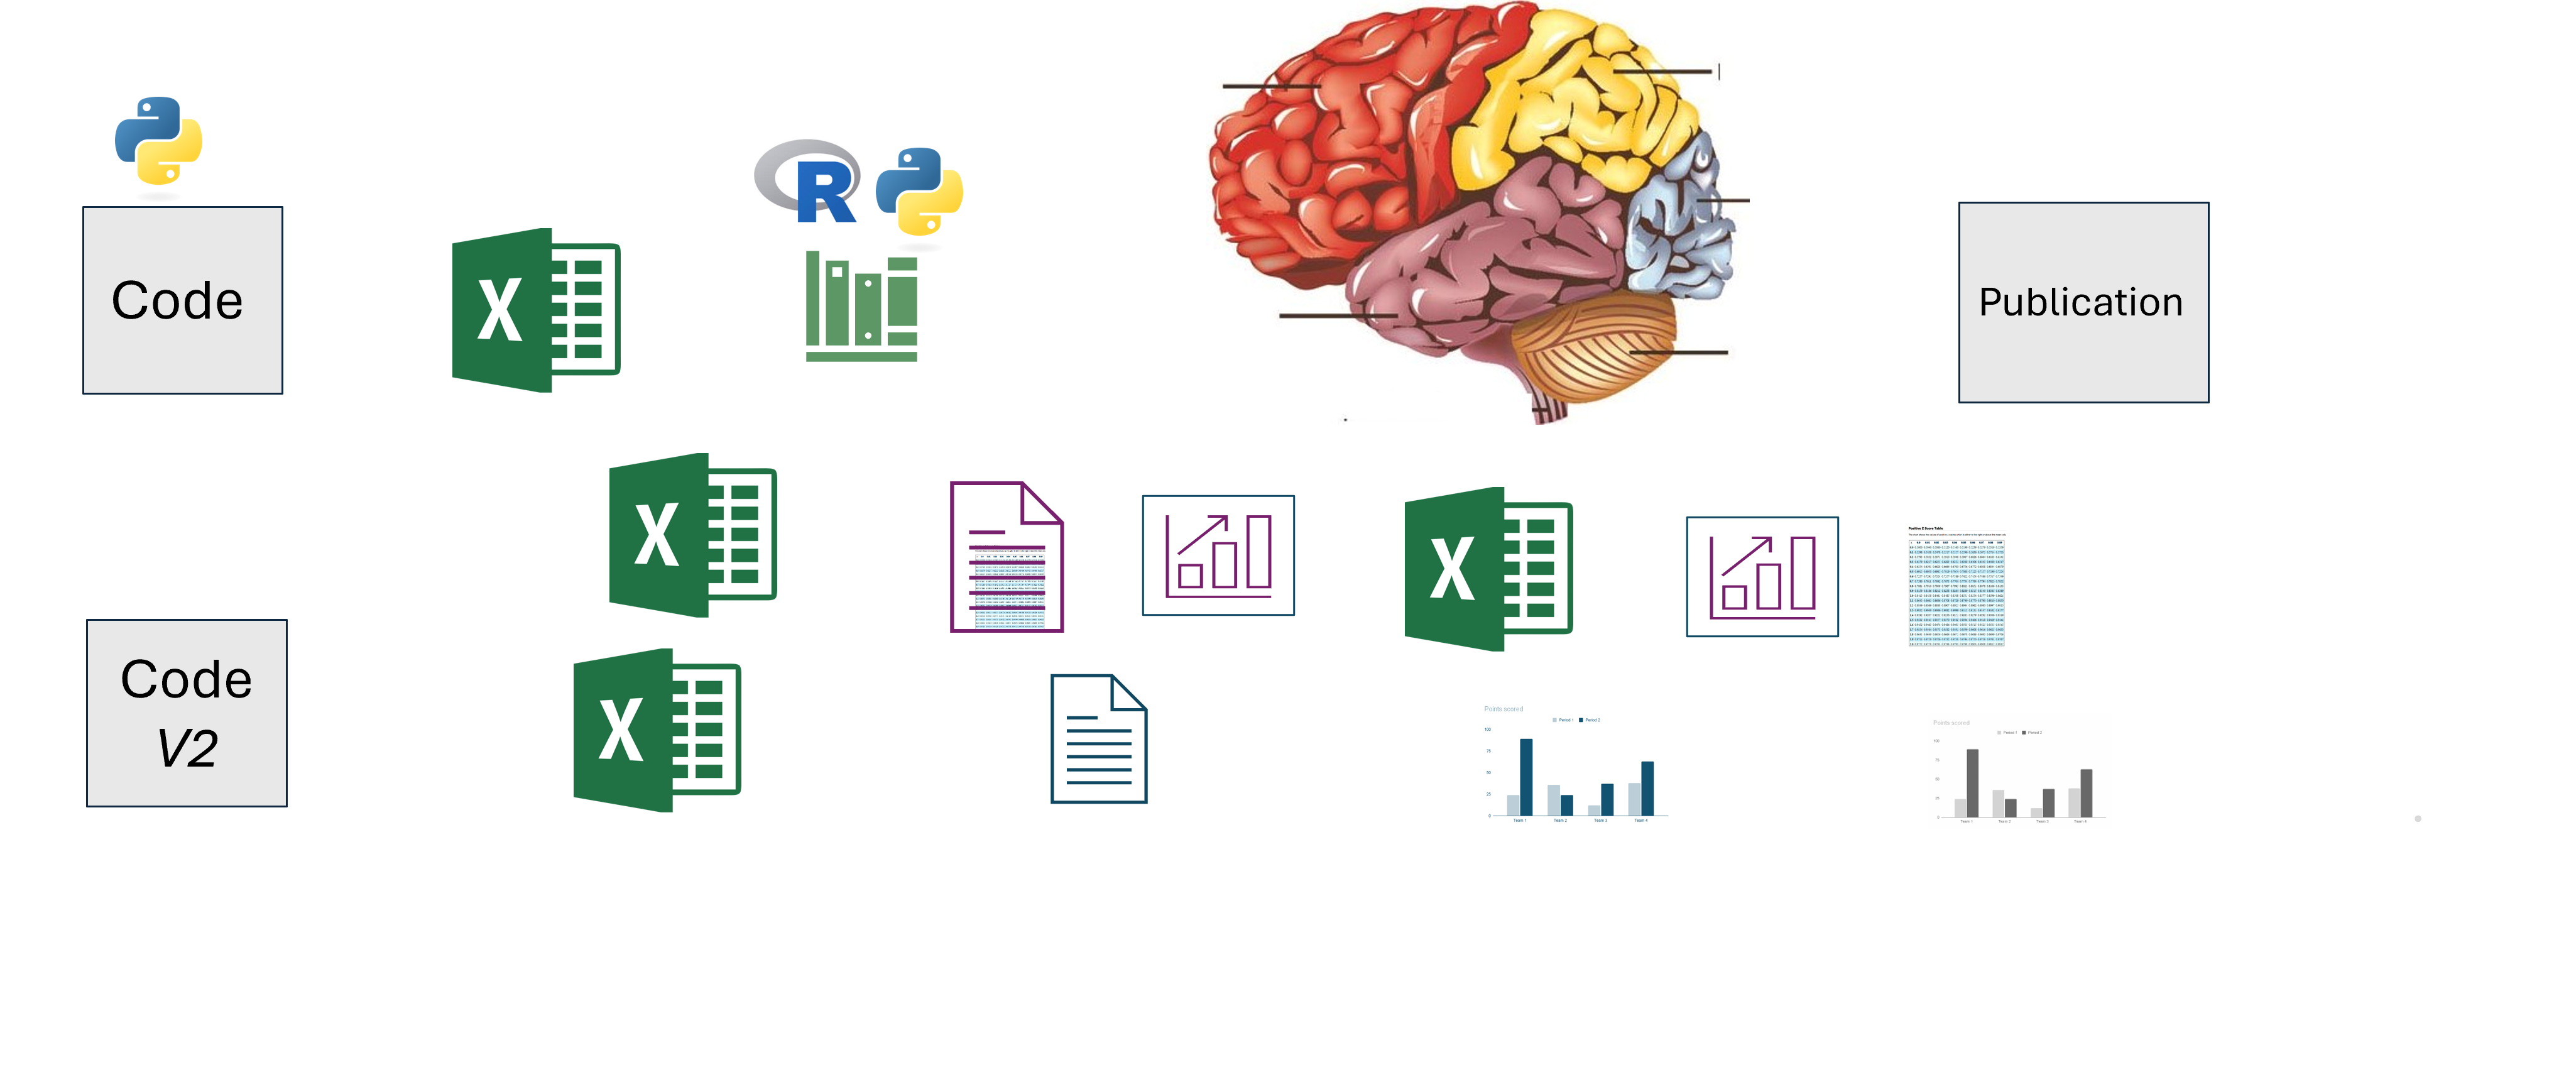
\includegraphics[width=1.0\textwidth]{Process15.png} }
        \only<4>{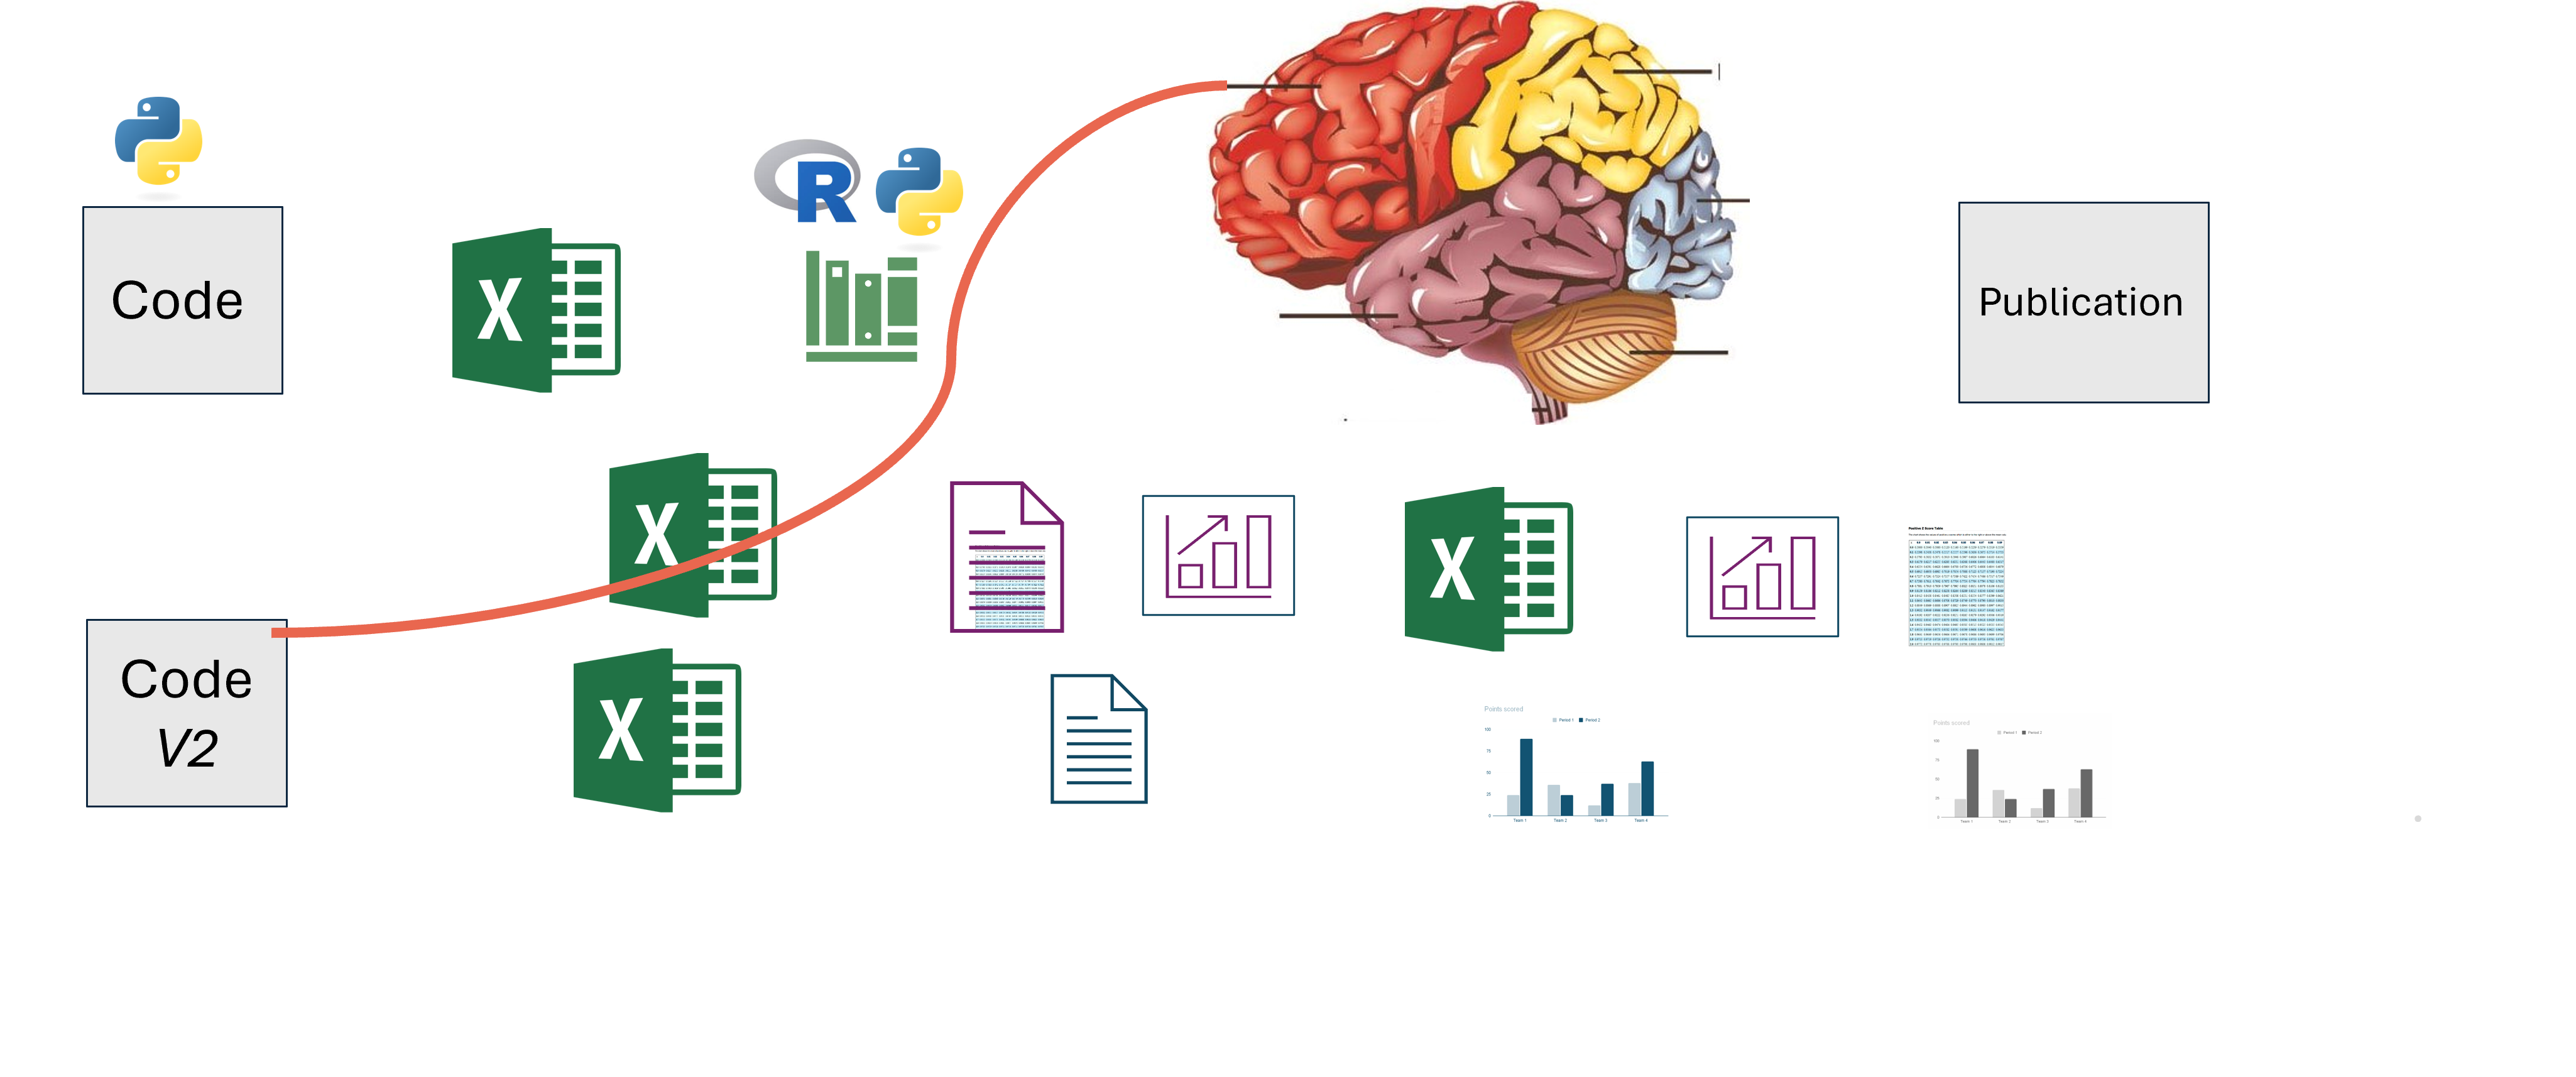
\includegraphics[width=1.0\textwidth]{Process16.png} }
        \only<5>{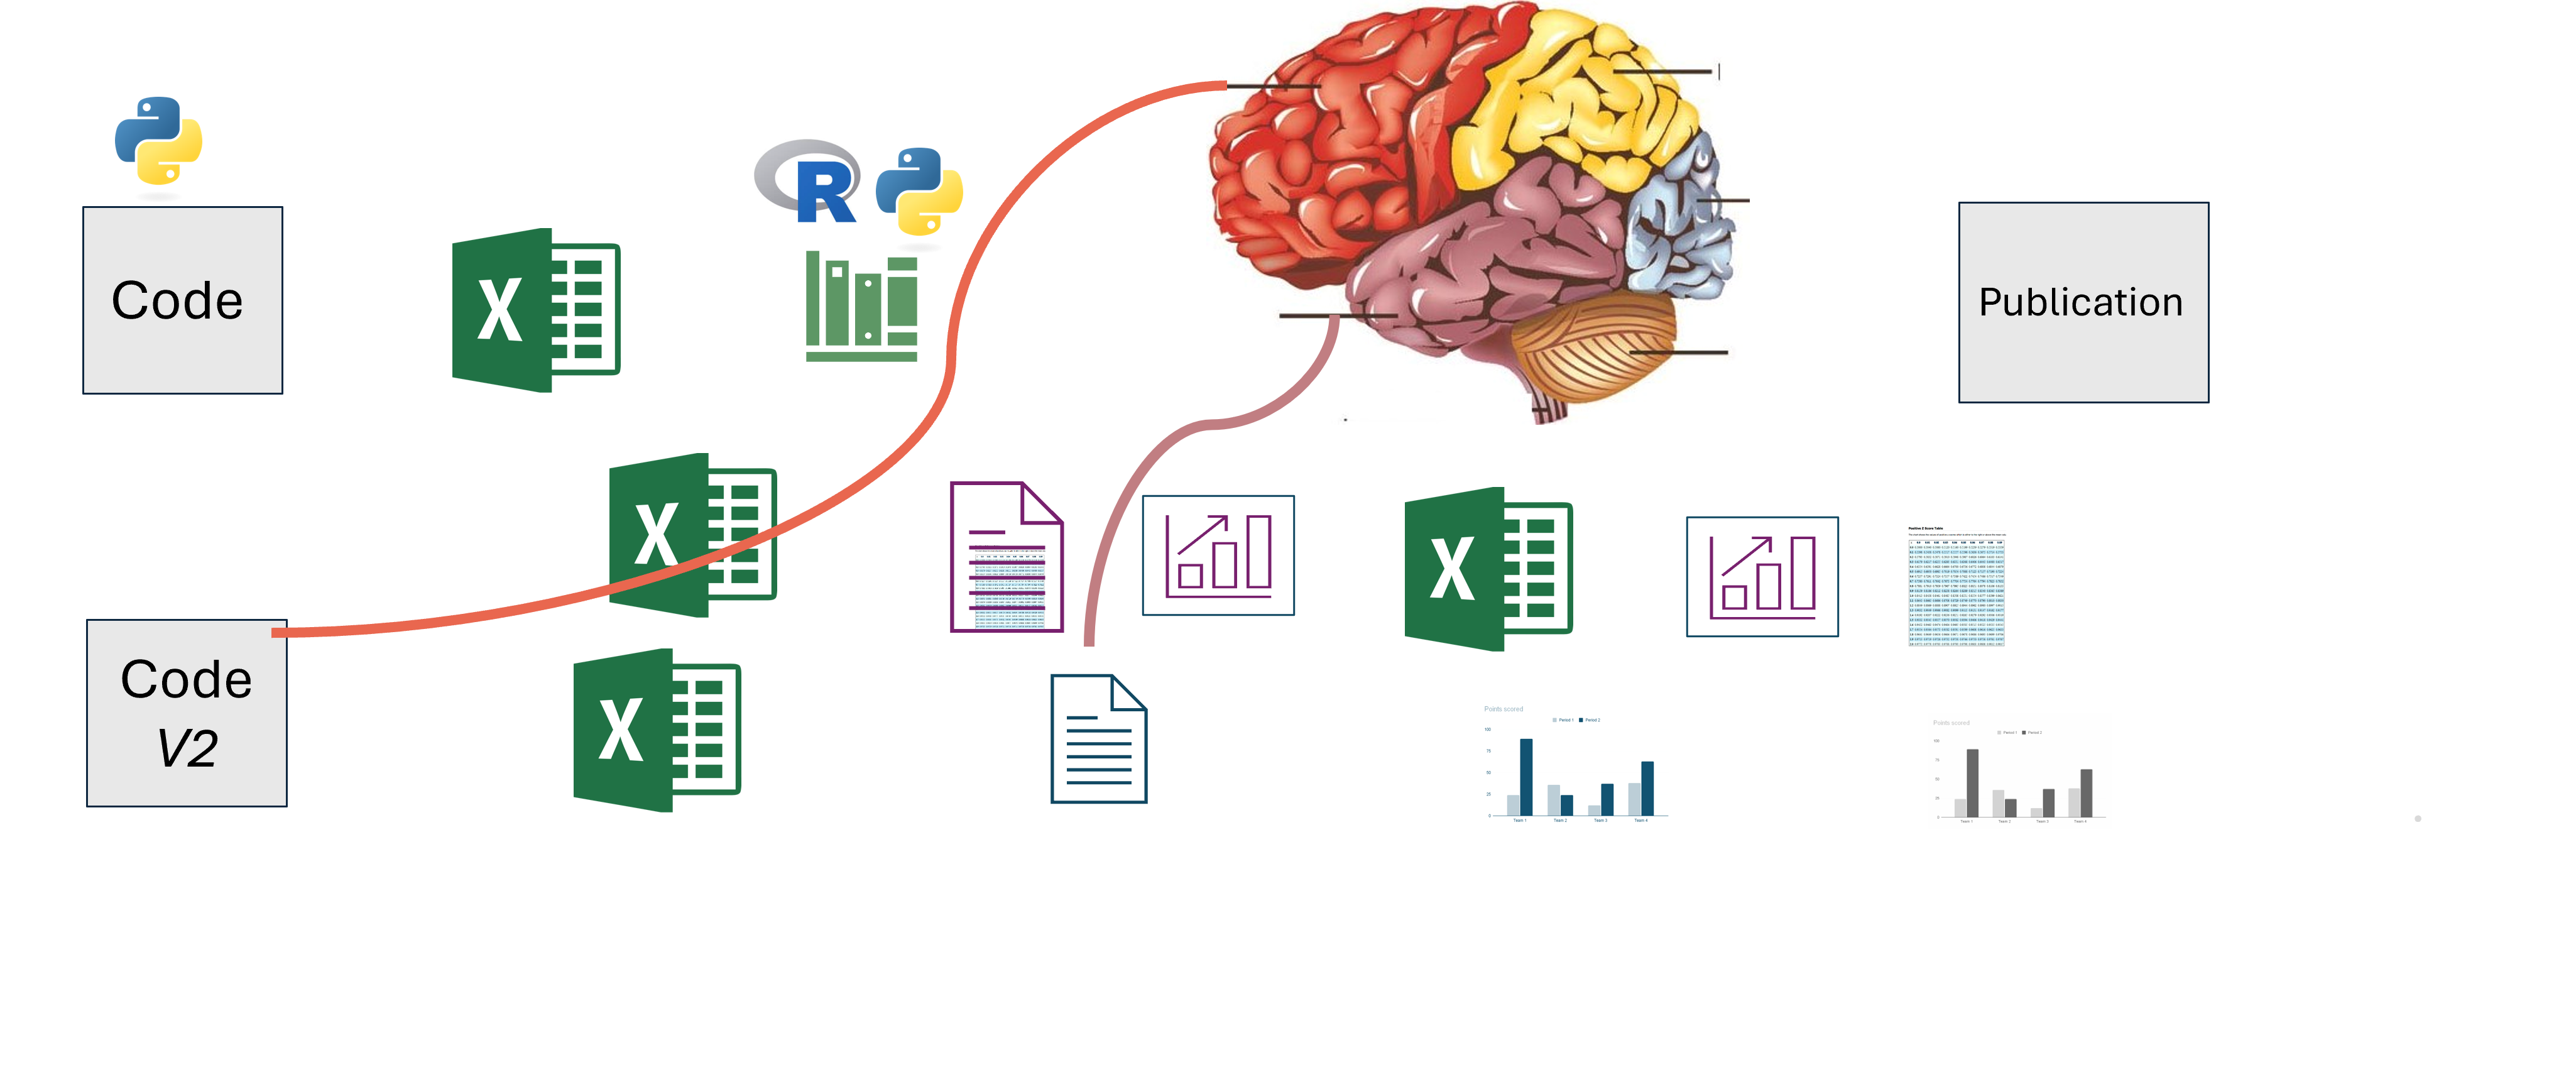
\includegraphics[width=1.0\textwidth]{Process17.png}}
        \only<6>{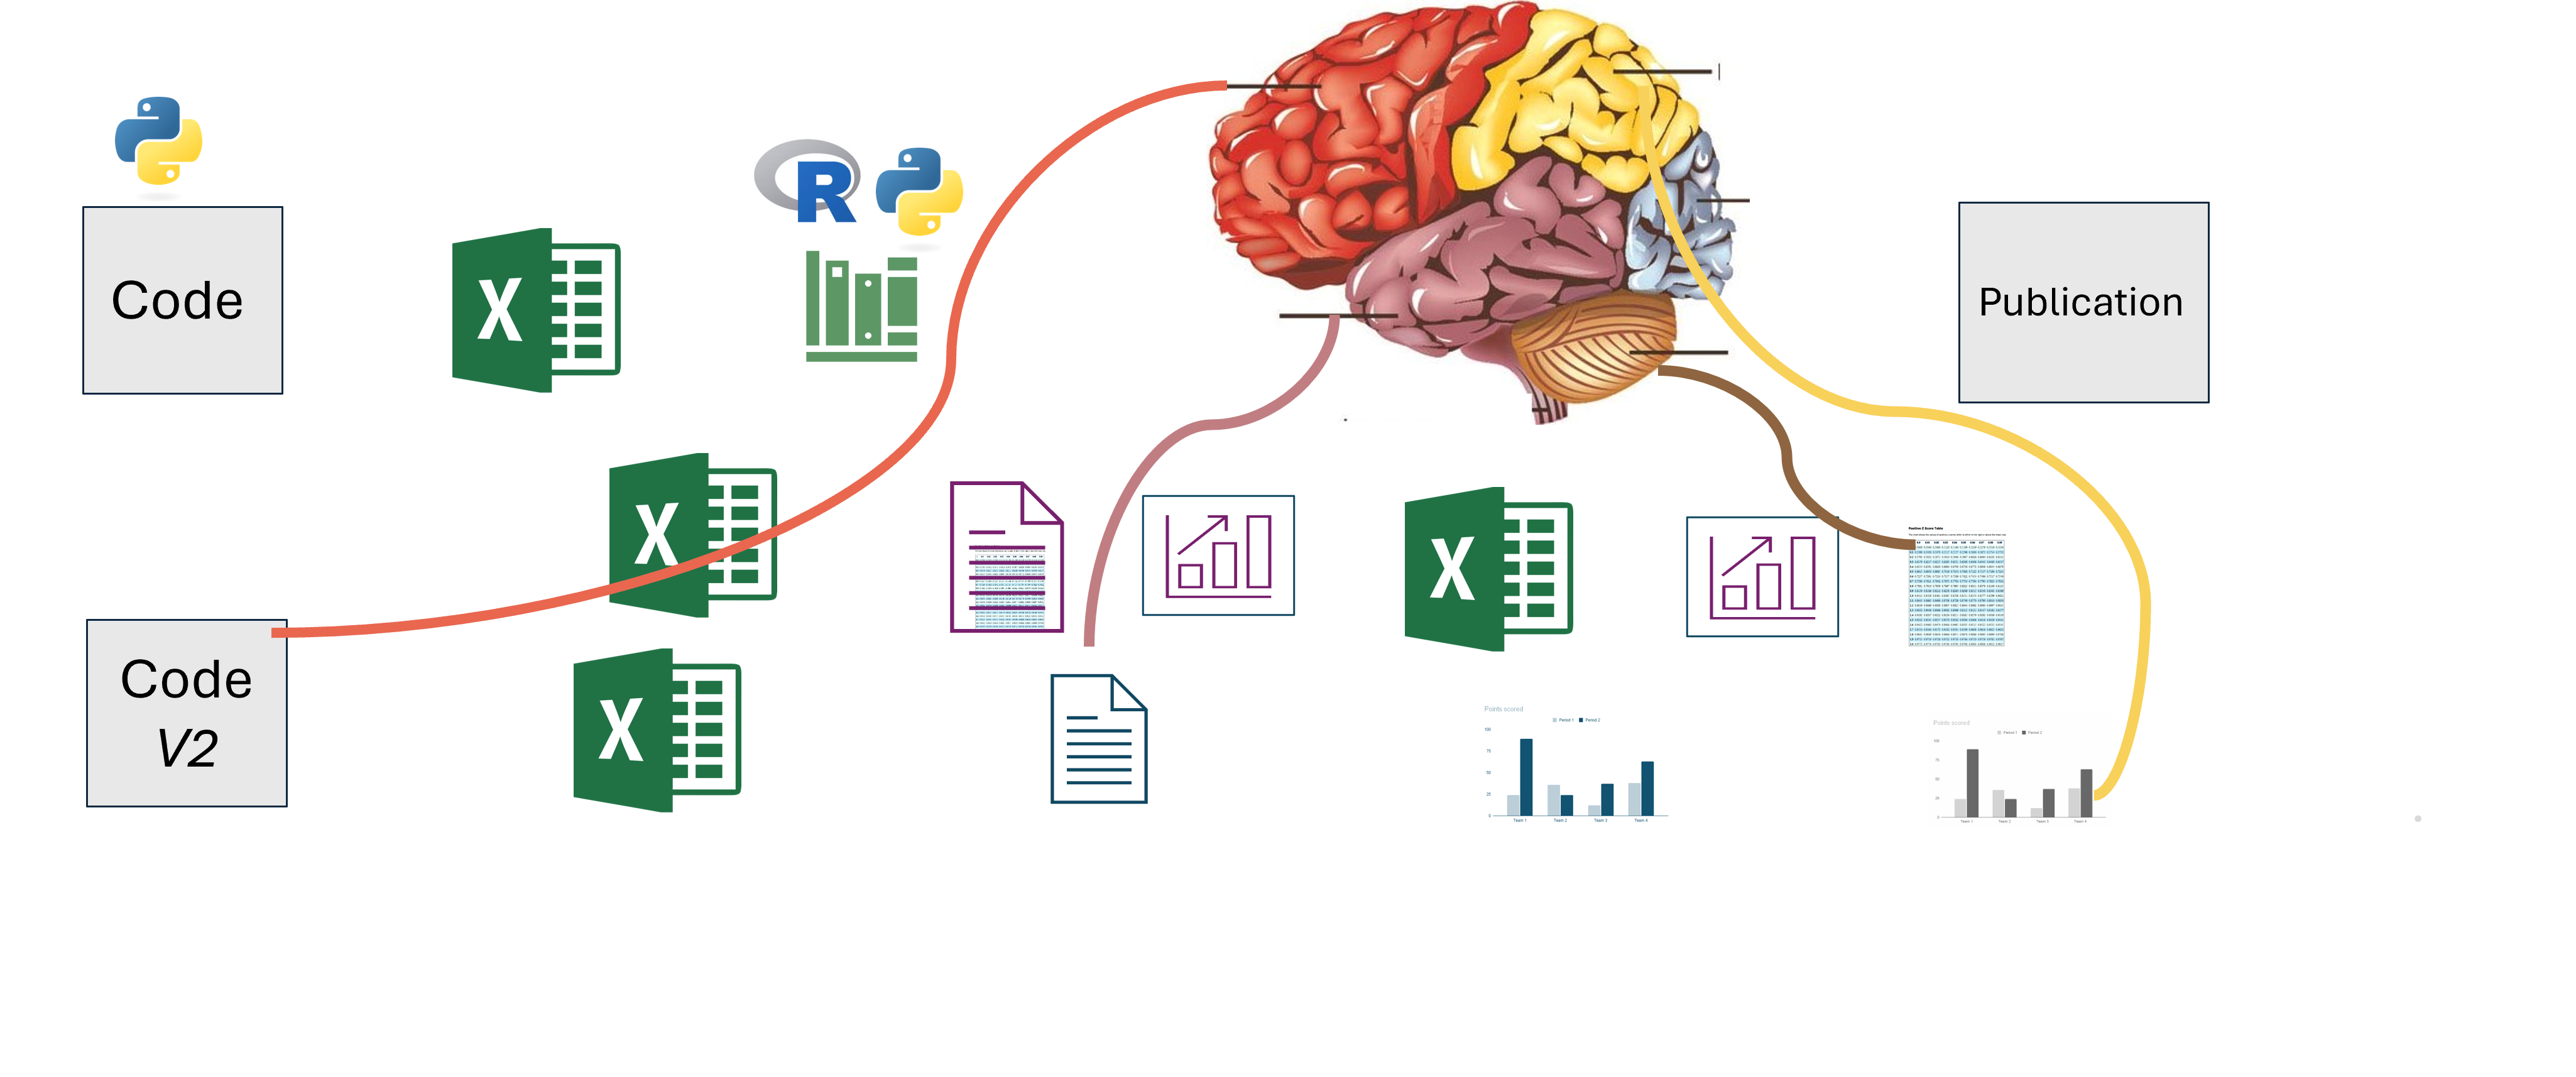
\includegraphics[width=1.0\textwidth]{Process18.png}}
        \only<7>{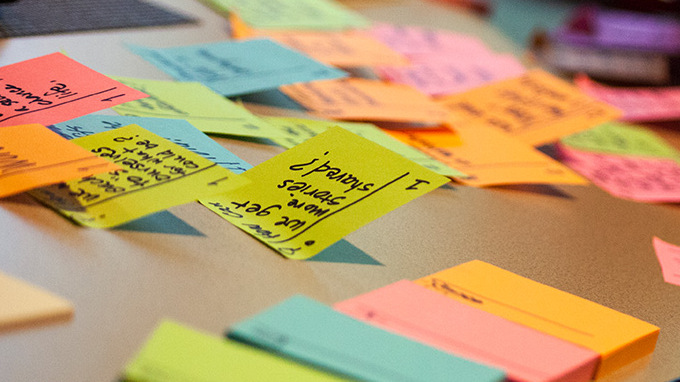
\includegraphics[width=1.0\textwidth]{Post-it.jpg} }
    \end{itemize}
    \end{column}
  \end{columns}
\end{frame}

\section{Issues}

\begin{frame}{What are the issues?}
  \begin{columns}[T]
    \begin{column}{0.5\textwidth}
      \begin{itemize}[<+->]
        \item Errors due to cut and paste
        \item Errors are difficult to track
        \item Each operator has his/her own approach
        \item Several versions of code may coexist
        \item The steps aren't recorded
        \item Reproducibility is not granted
       % \item Quality control is hard
      \end{itemize}
    \end{column}
    \begin{column}{0.5\textwidth}
    \begin{itemize}
        \item[]  \only<1-2>{\href{https://www.bbc.com/news/technology-54423988}{ 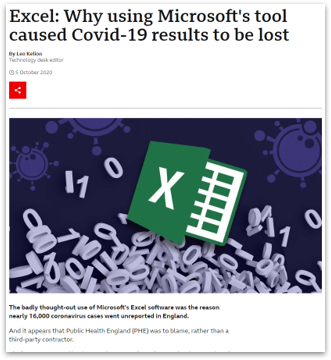
\includegraphics[width=1.0\textwidth]{ExcelUK.png}}}
         \only<3>{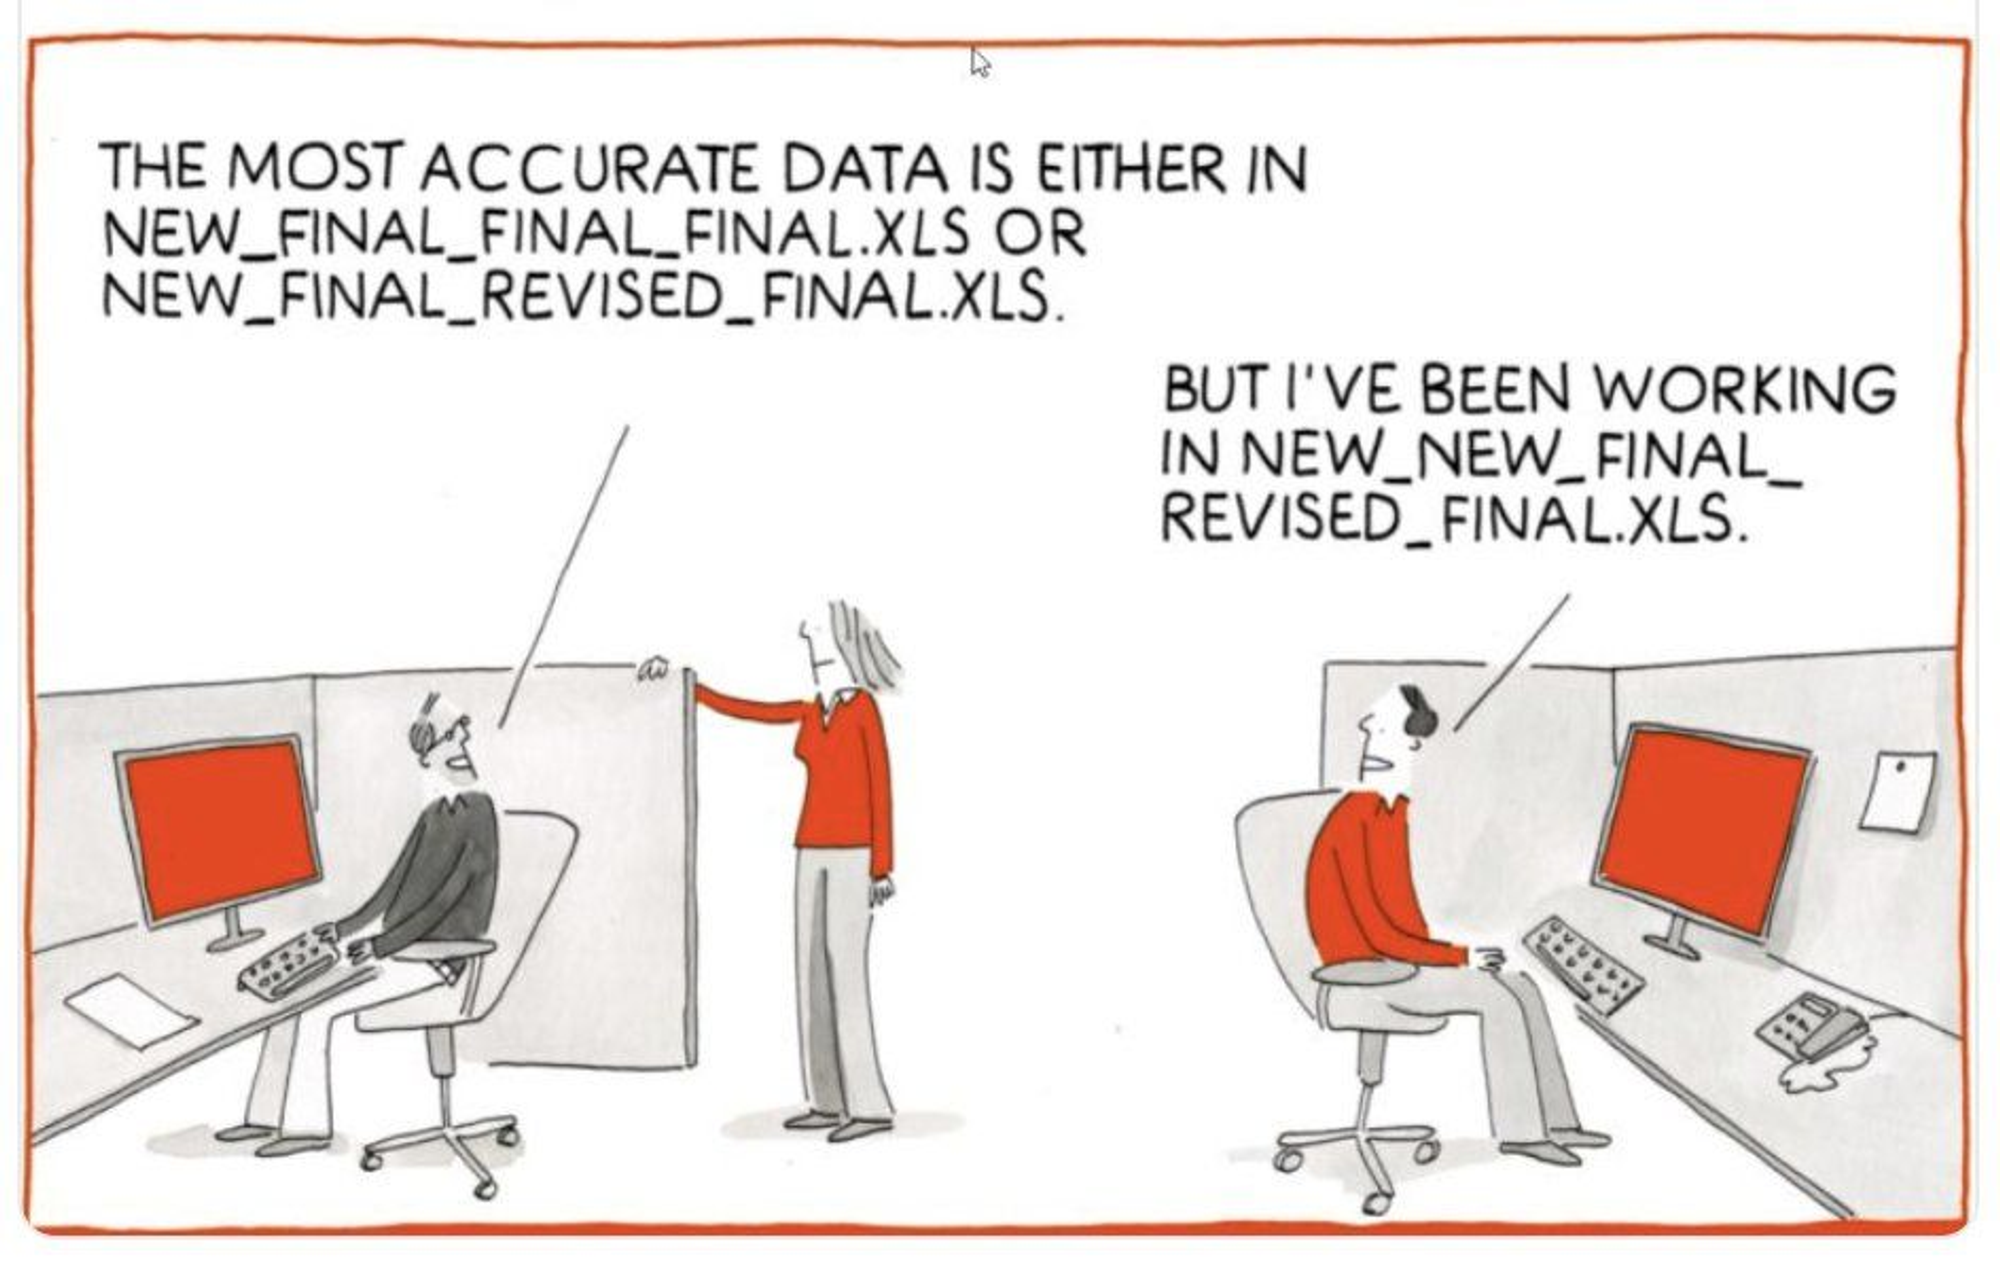
\includegraphics[width=1.0\textwidth]{FinalFinalVersion.png}}
         \only<4-5>{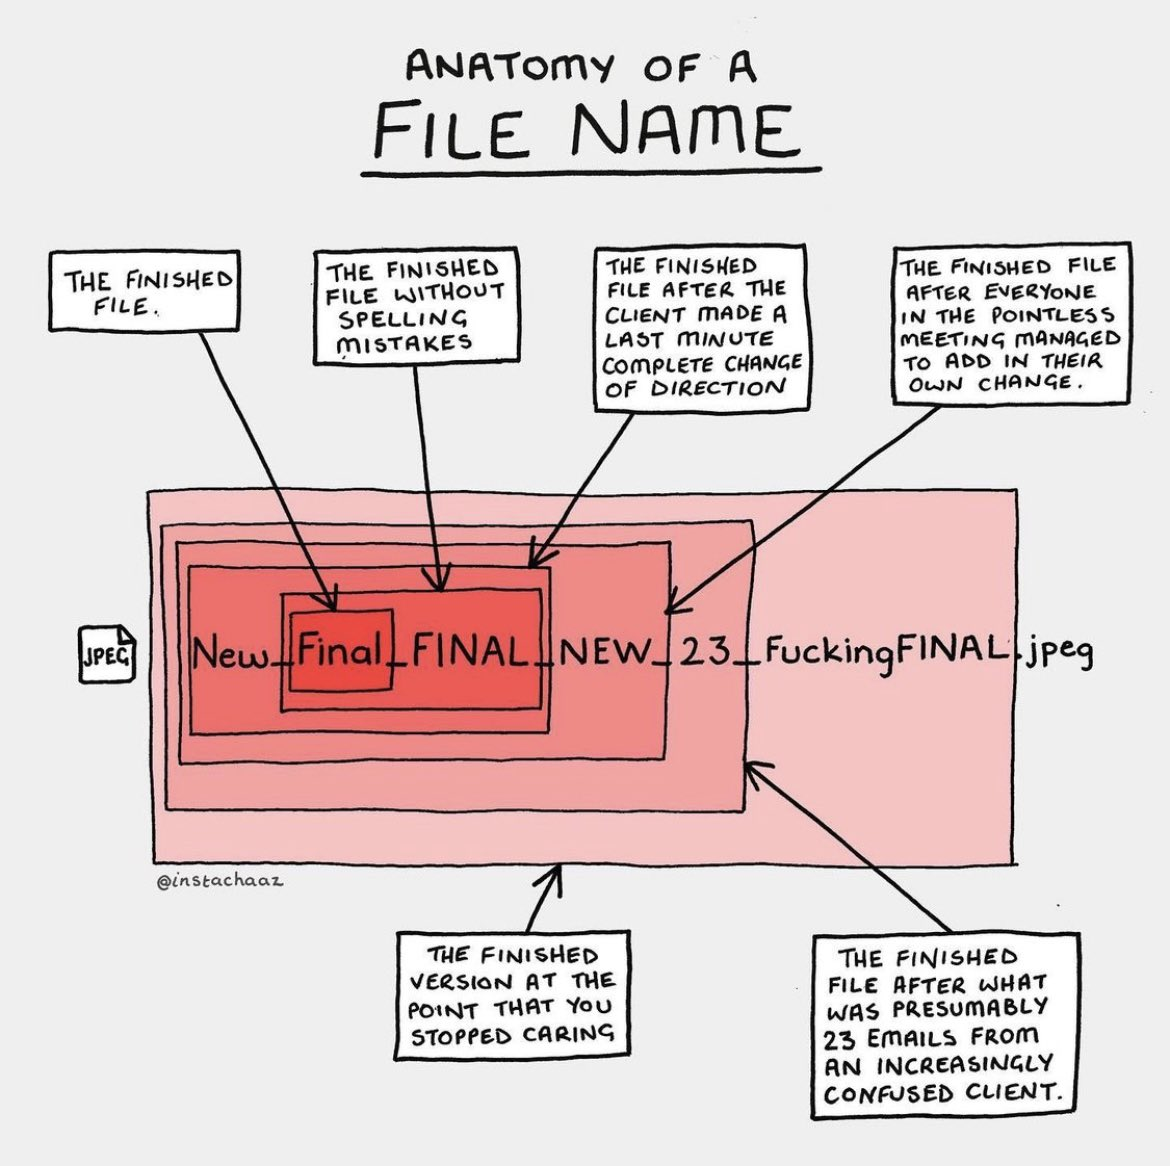
\includegraphics[width=1.0\textwidth]{AnatomyOfaFile.png}}
         \only<6>{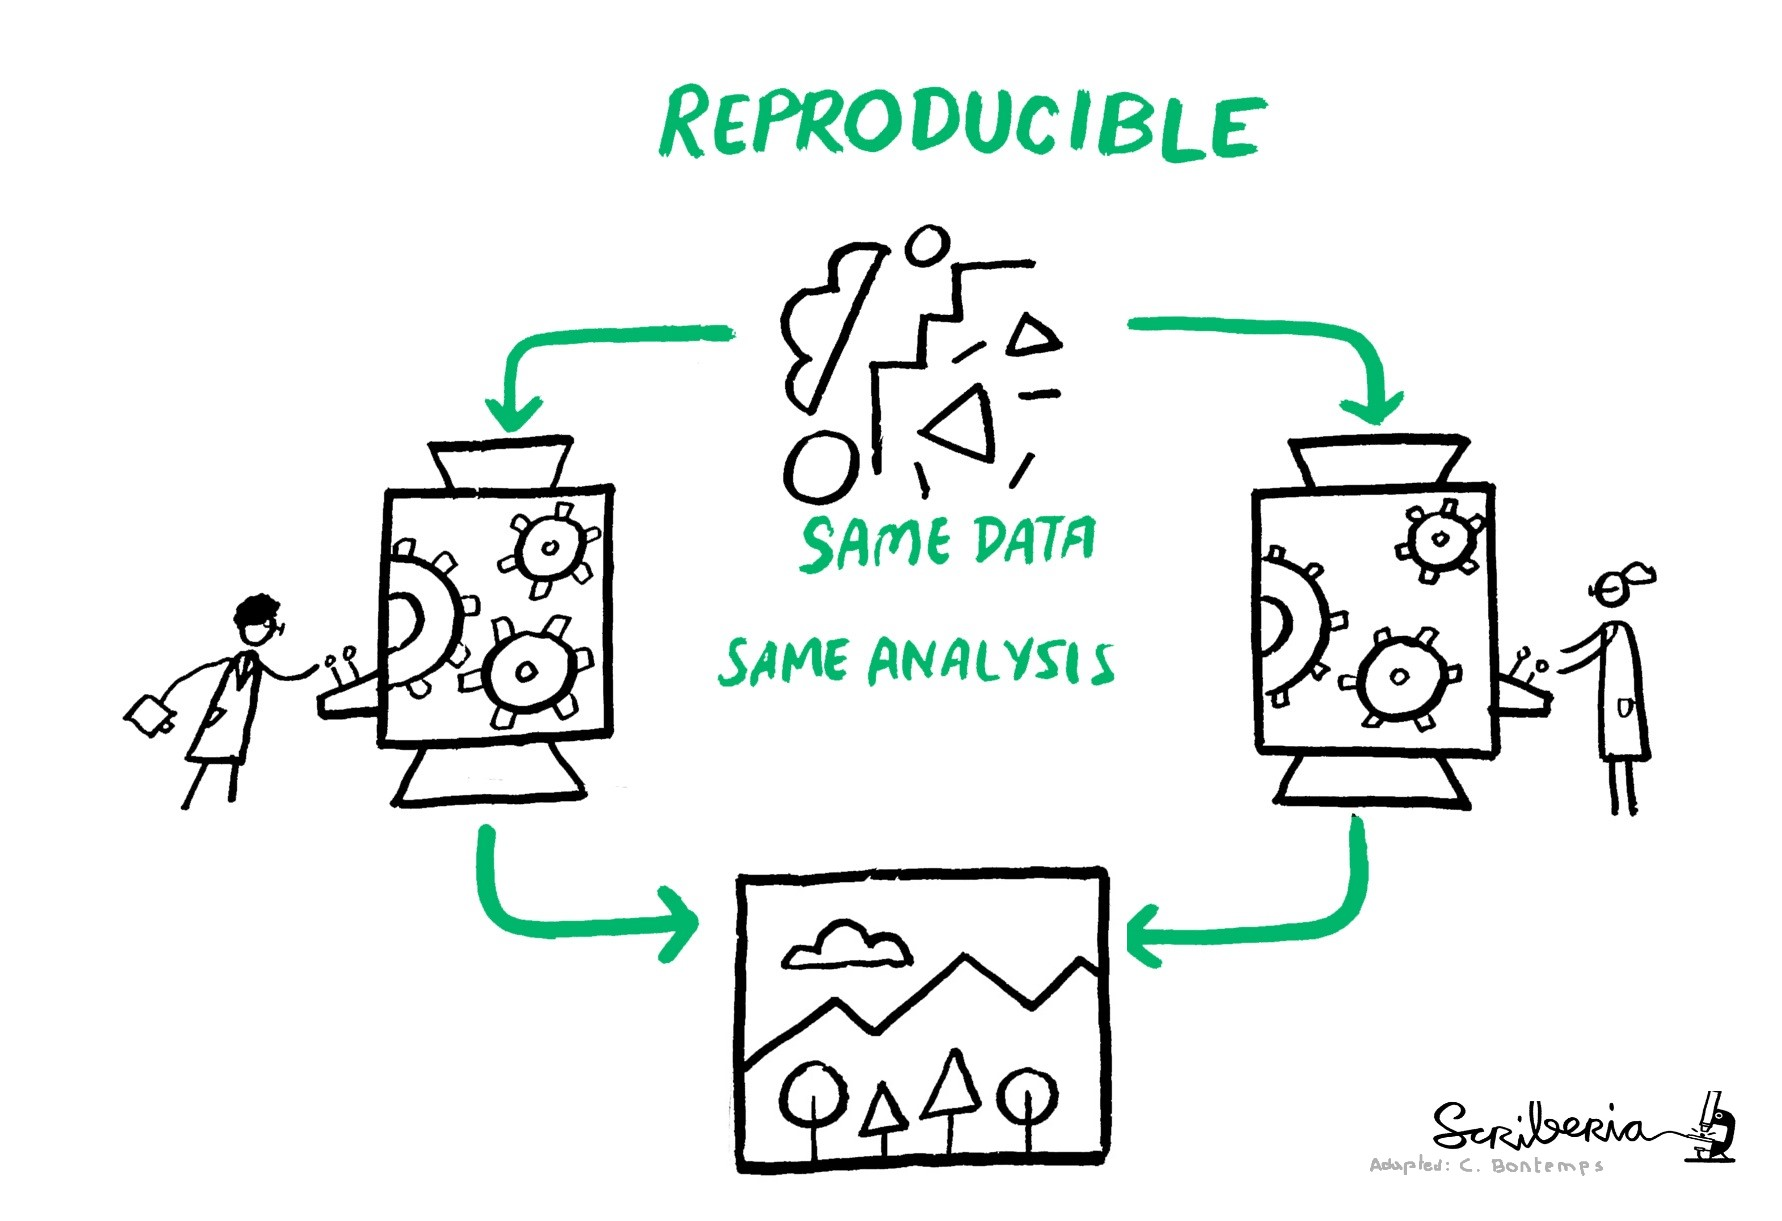
\includegraphics[width=1.0\textwidth]{Reproducible.jpg}}
         \end{itemize}
    \end{column}
  \end{columns}
\end{frame}

% Other slides should go here...

\section{RAP}  % Better practices

\begin{frame}{What is A Reproducible Analytical Pipeline?}
  \begin{columns}[T]
    \begin{column}{0.5\textwidth}
      \begin{itemize}[<+->]
        \item It is a process % or a way to think a process 
        \item It is automated 
        \item It is easily reproducible                 
        \item It minimises mistakes      
        \item It is fast                 
        \item It builds trust            
      \end{itemize}
    \end{column}
    \begin{column}{0.5\textwidth}
    \begin{itemize}
        \item[] 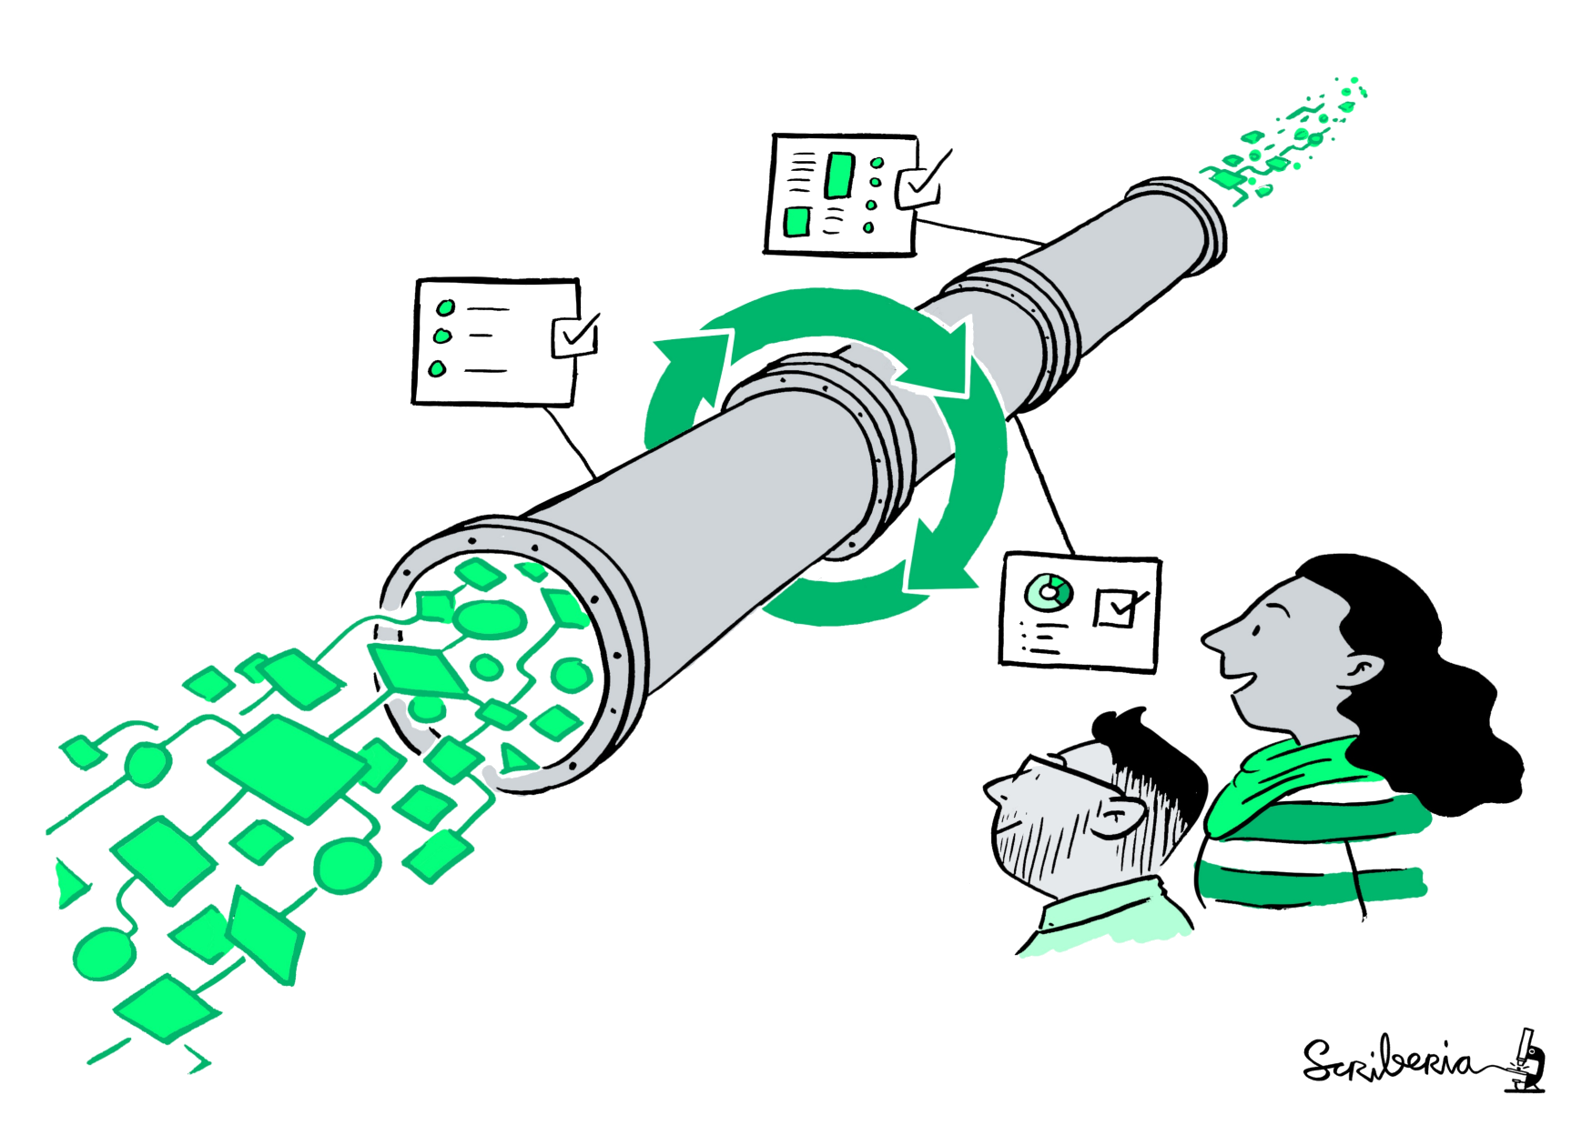
\includegraphics[width=1.0\textwidth]{ReusablePipeline.png}
    \end{itemize}
    \end{column}
  \end{columns}
\end{frame}

\begin{frame}{What does a RAP look like?}
 \begin{center}
  \begin{itemize}
        \only<1>{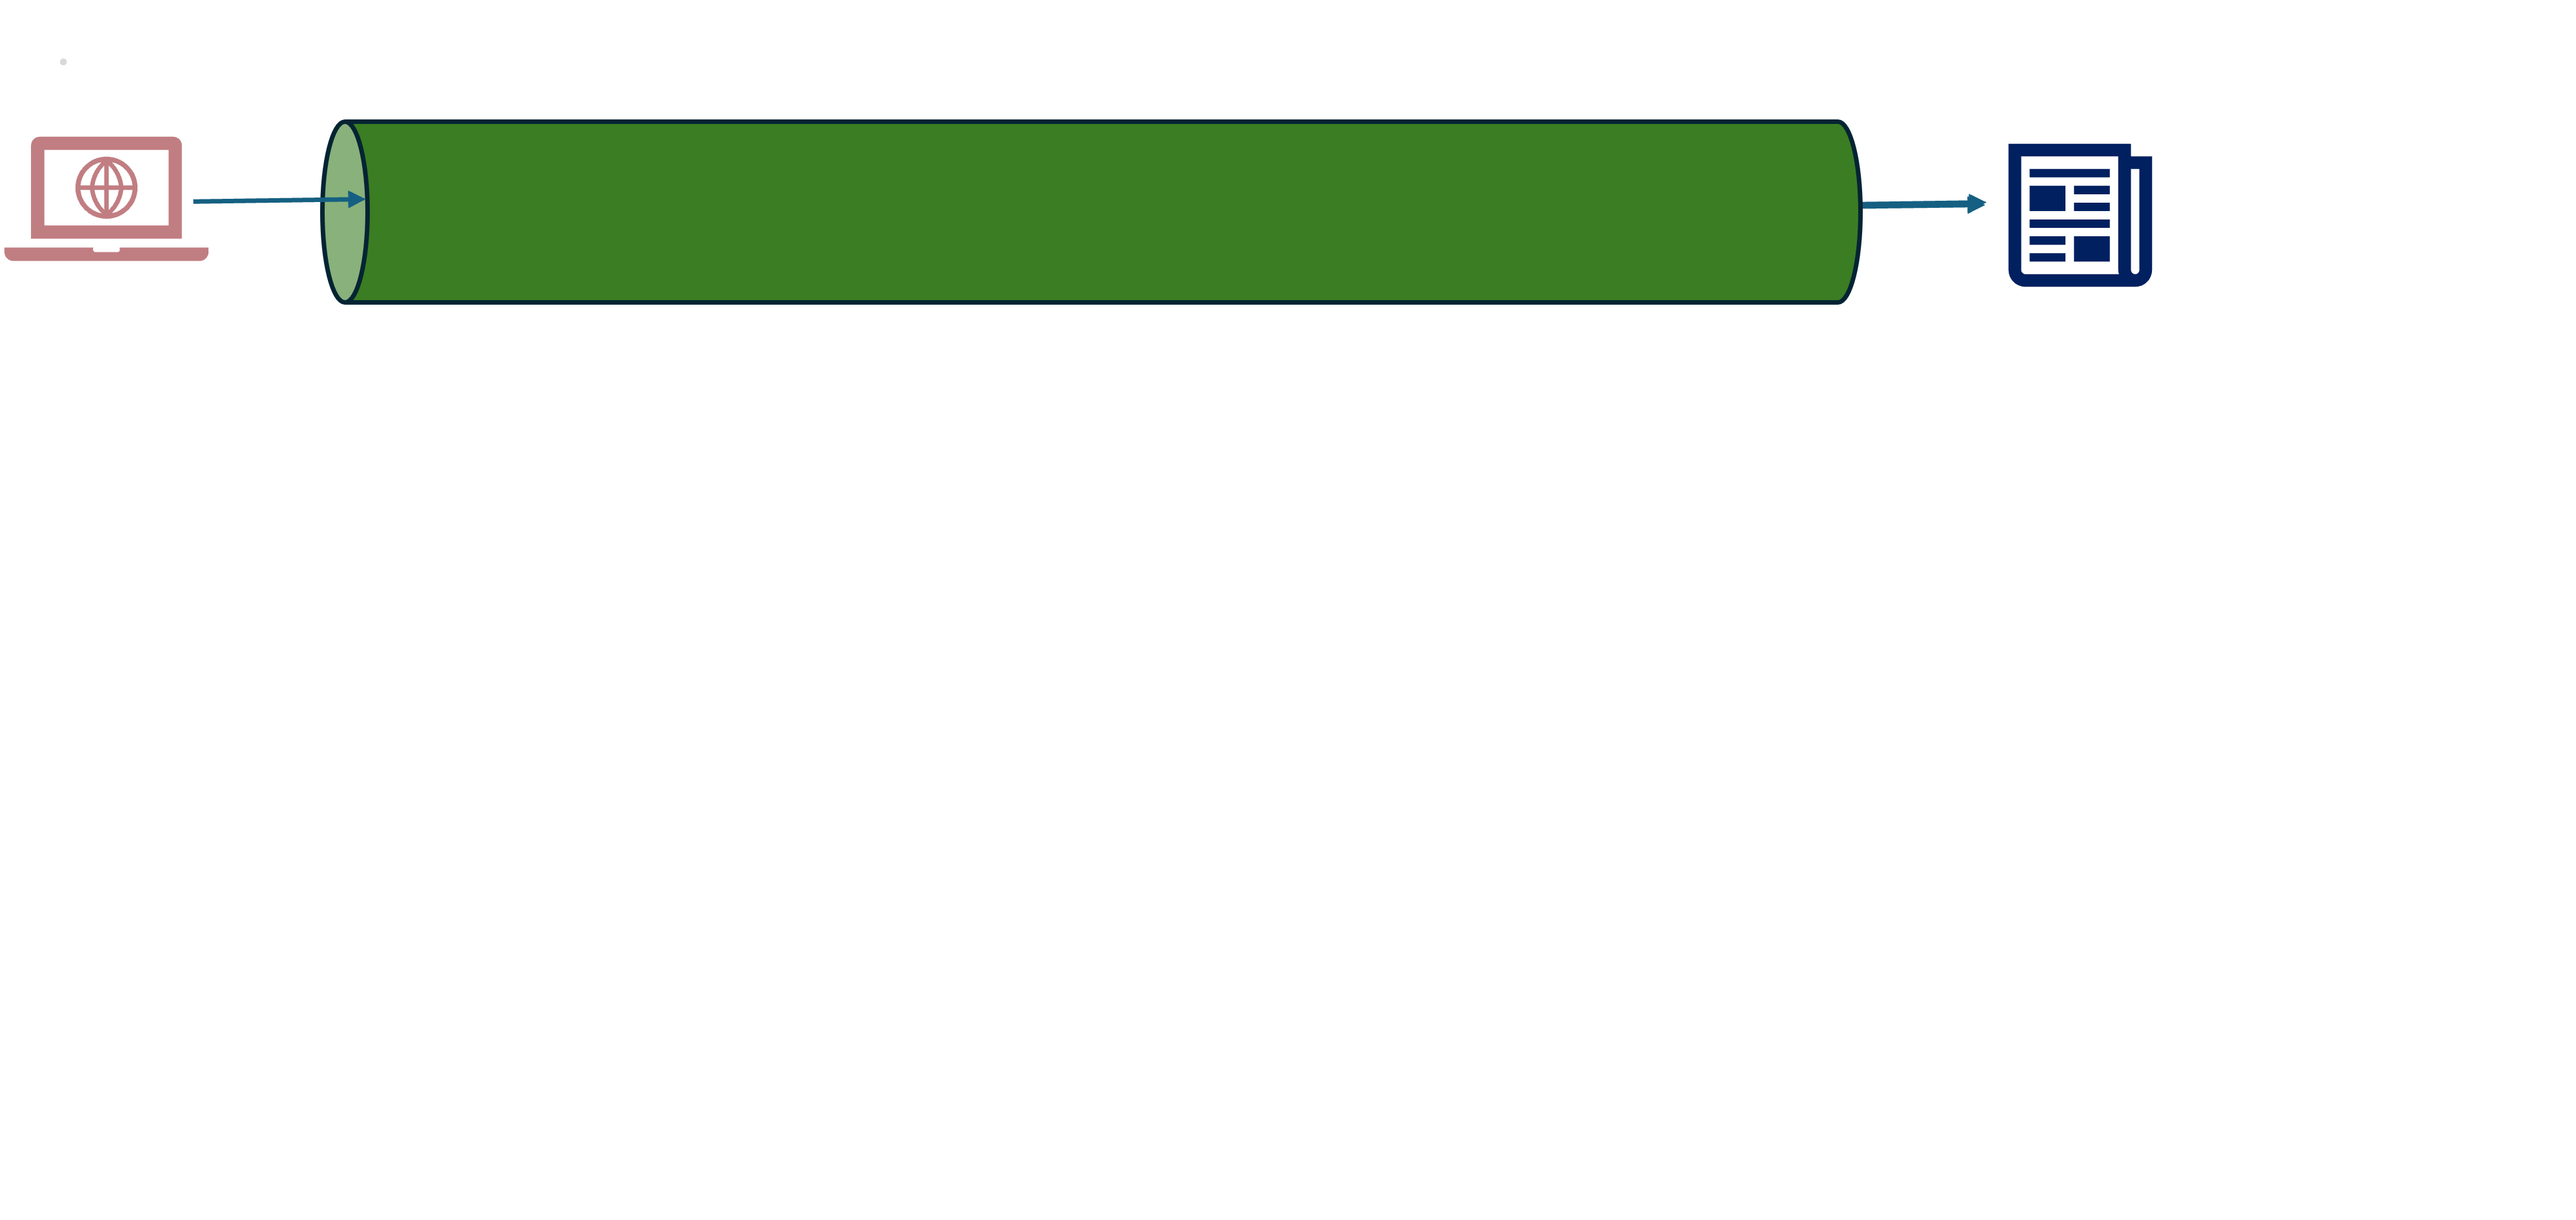
\includegraphics[width=0.8\textwidth]{Pipeline1.png} \\ Comment 1}
        \only<2>{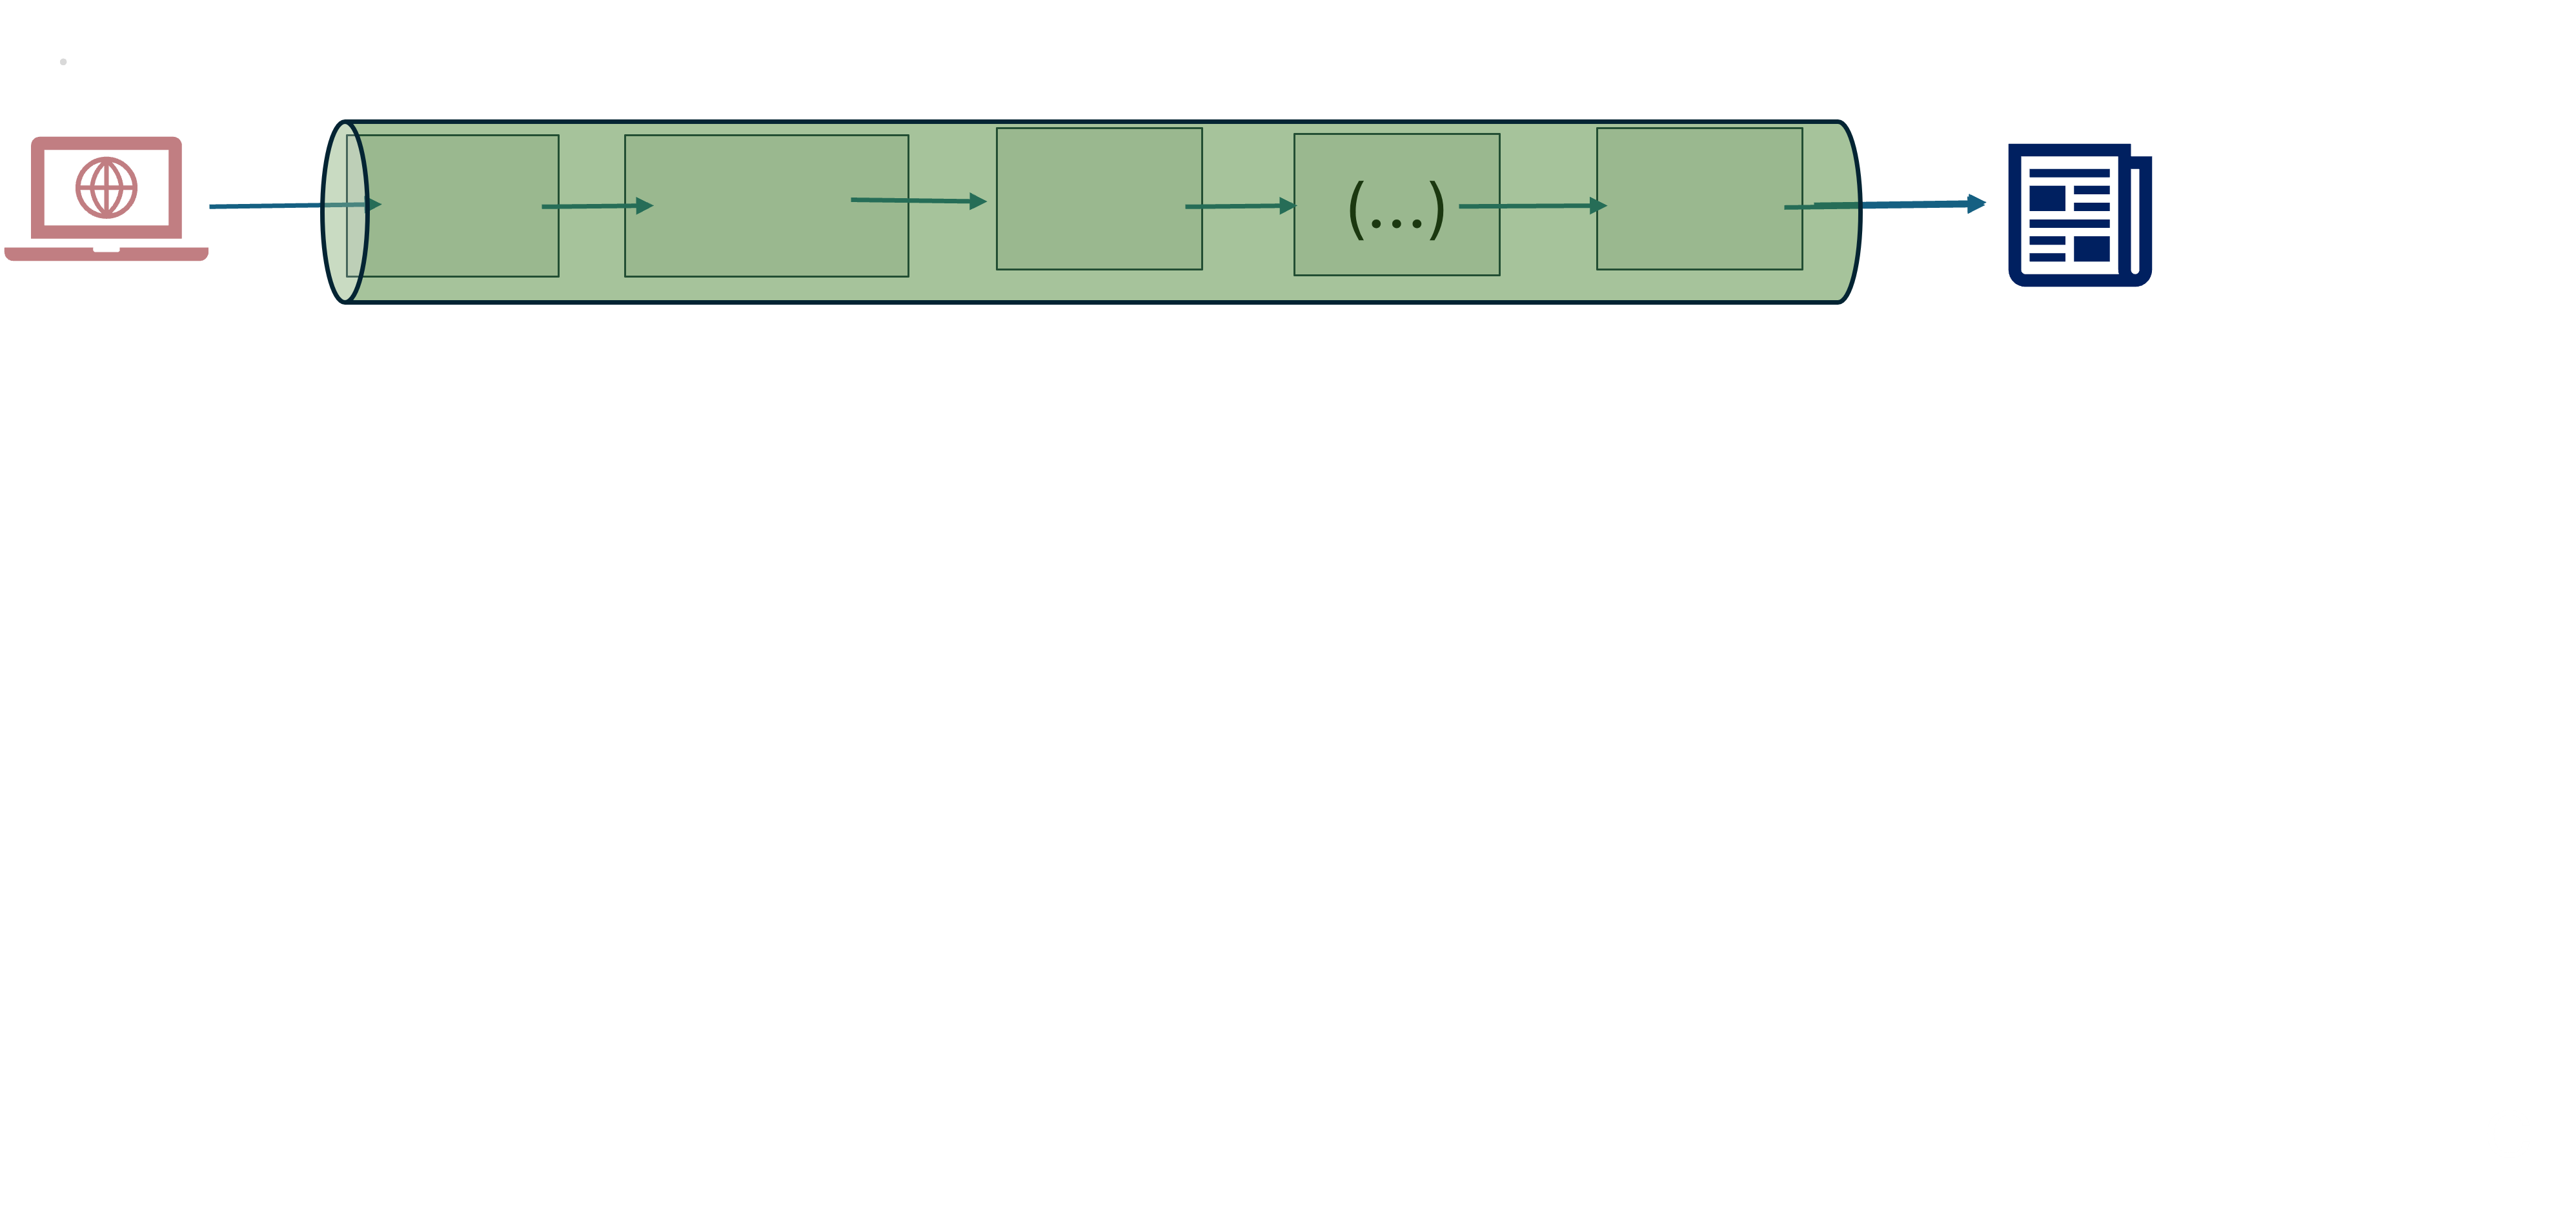
\includegraphics[width=0.8\textwidth]{Pipeline2.png} \\ Comment 2}
        \only<3>{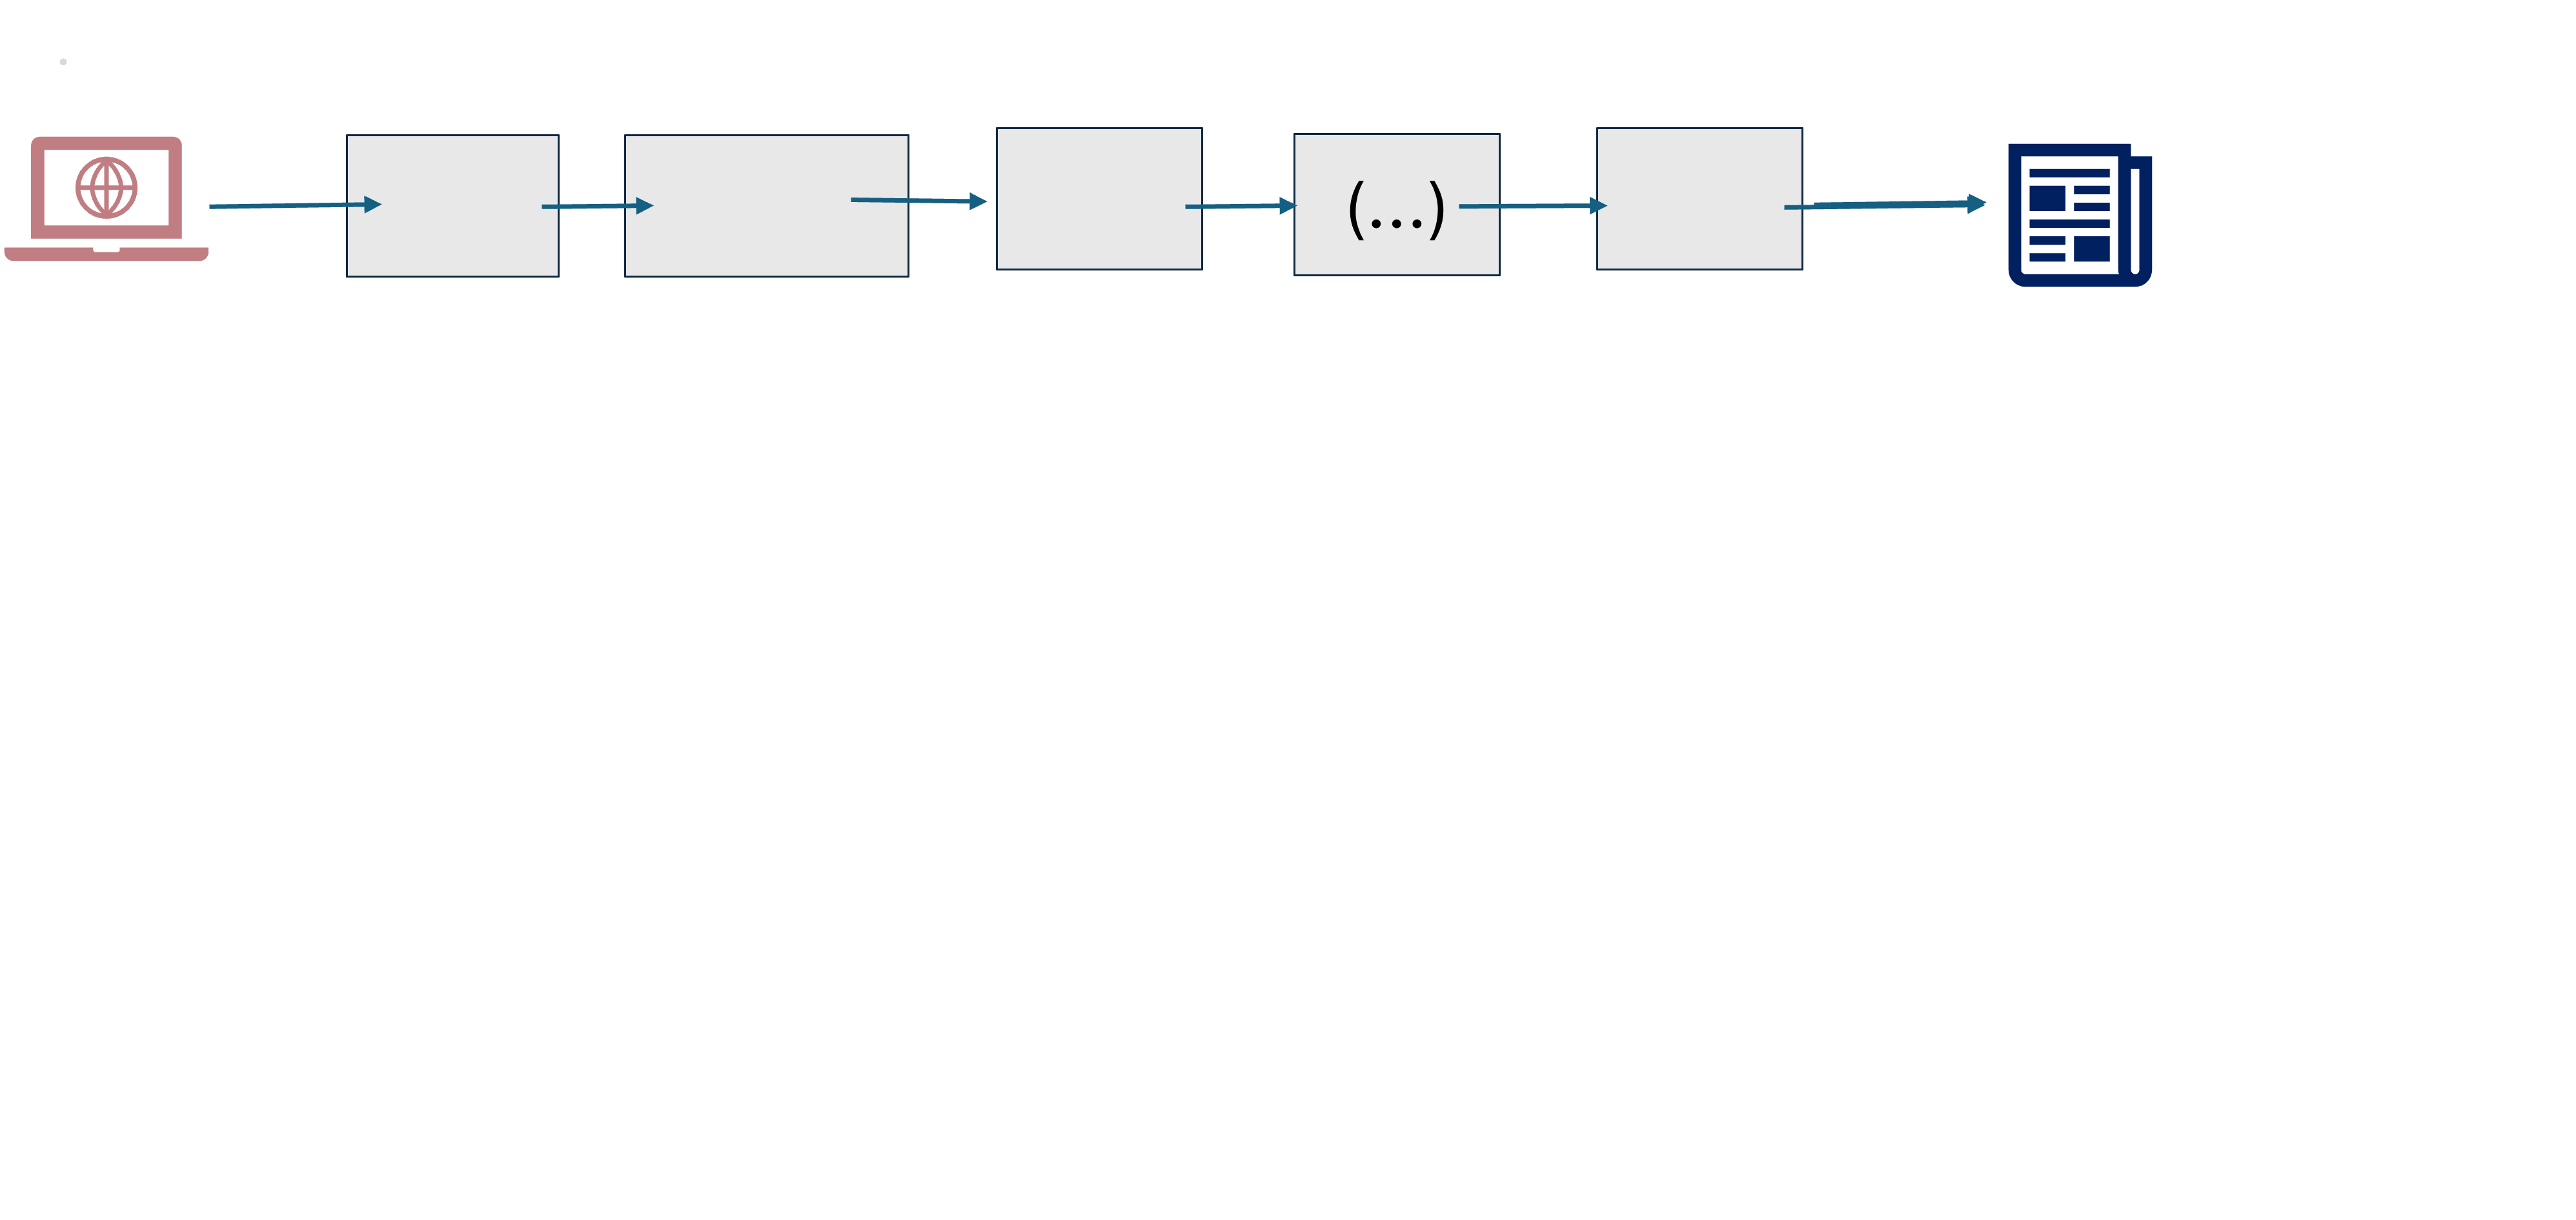
\includegraphics[width=0.8\textwidth]{Pipeline3.png} \\ Comment 3}
        \only<4>{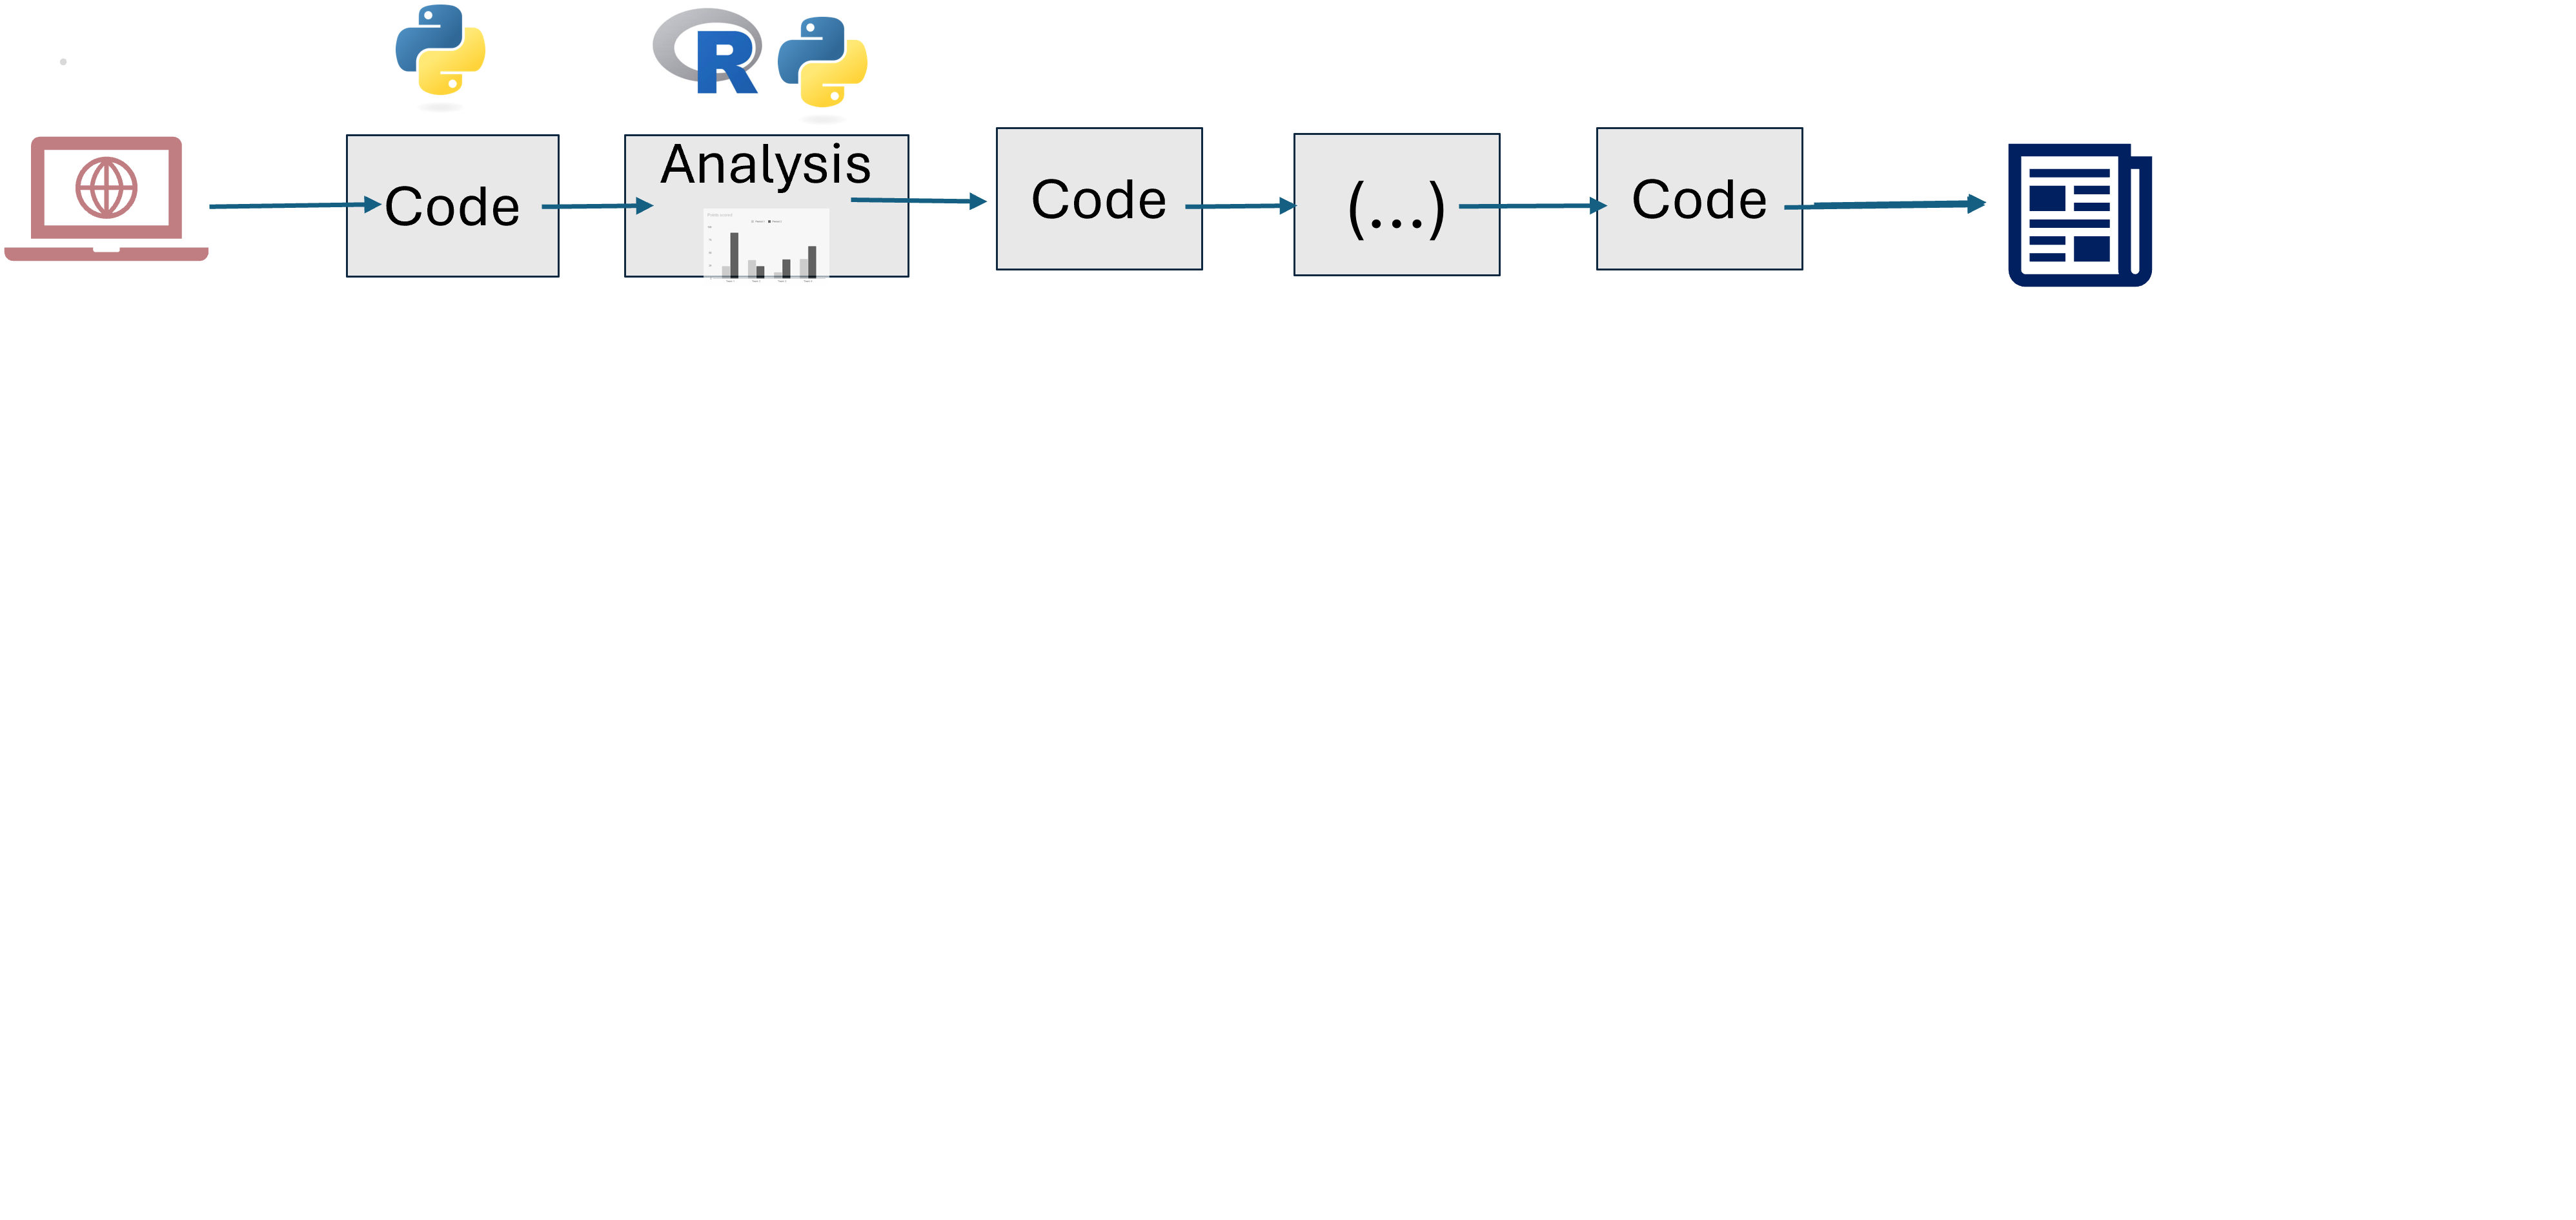
\includegraphics[width=0.8\textwidth]{Pipeline4.png} \\ Comment 4}
        \only<5>{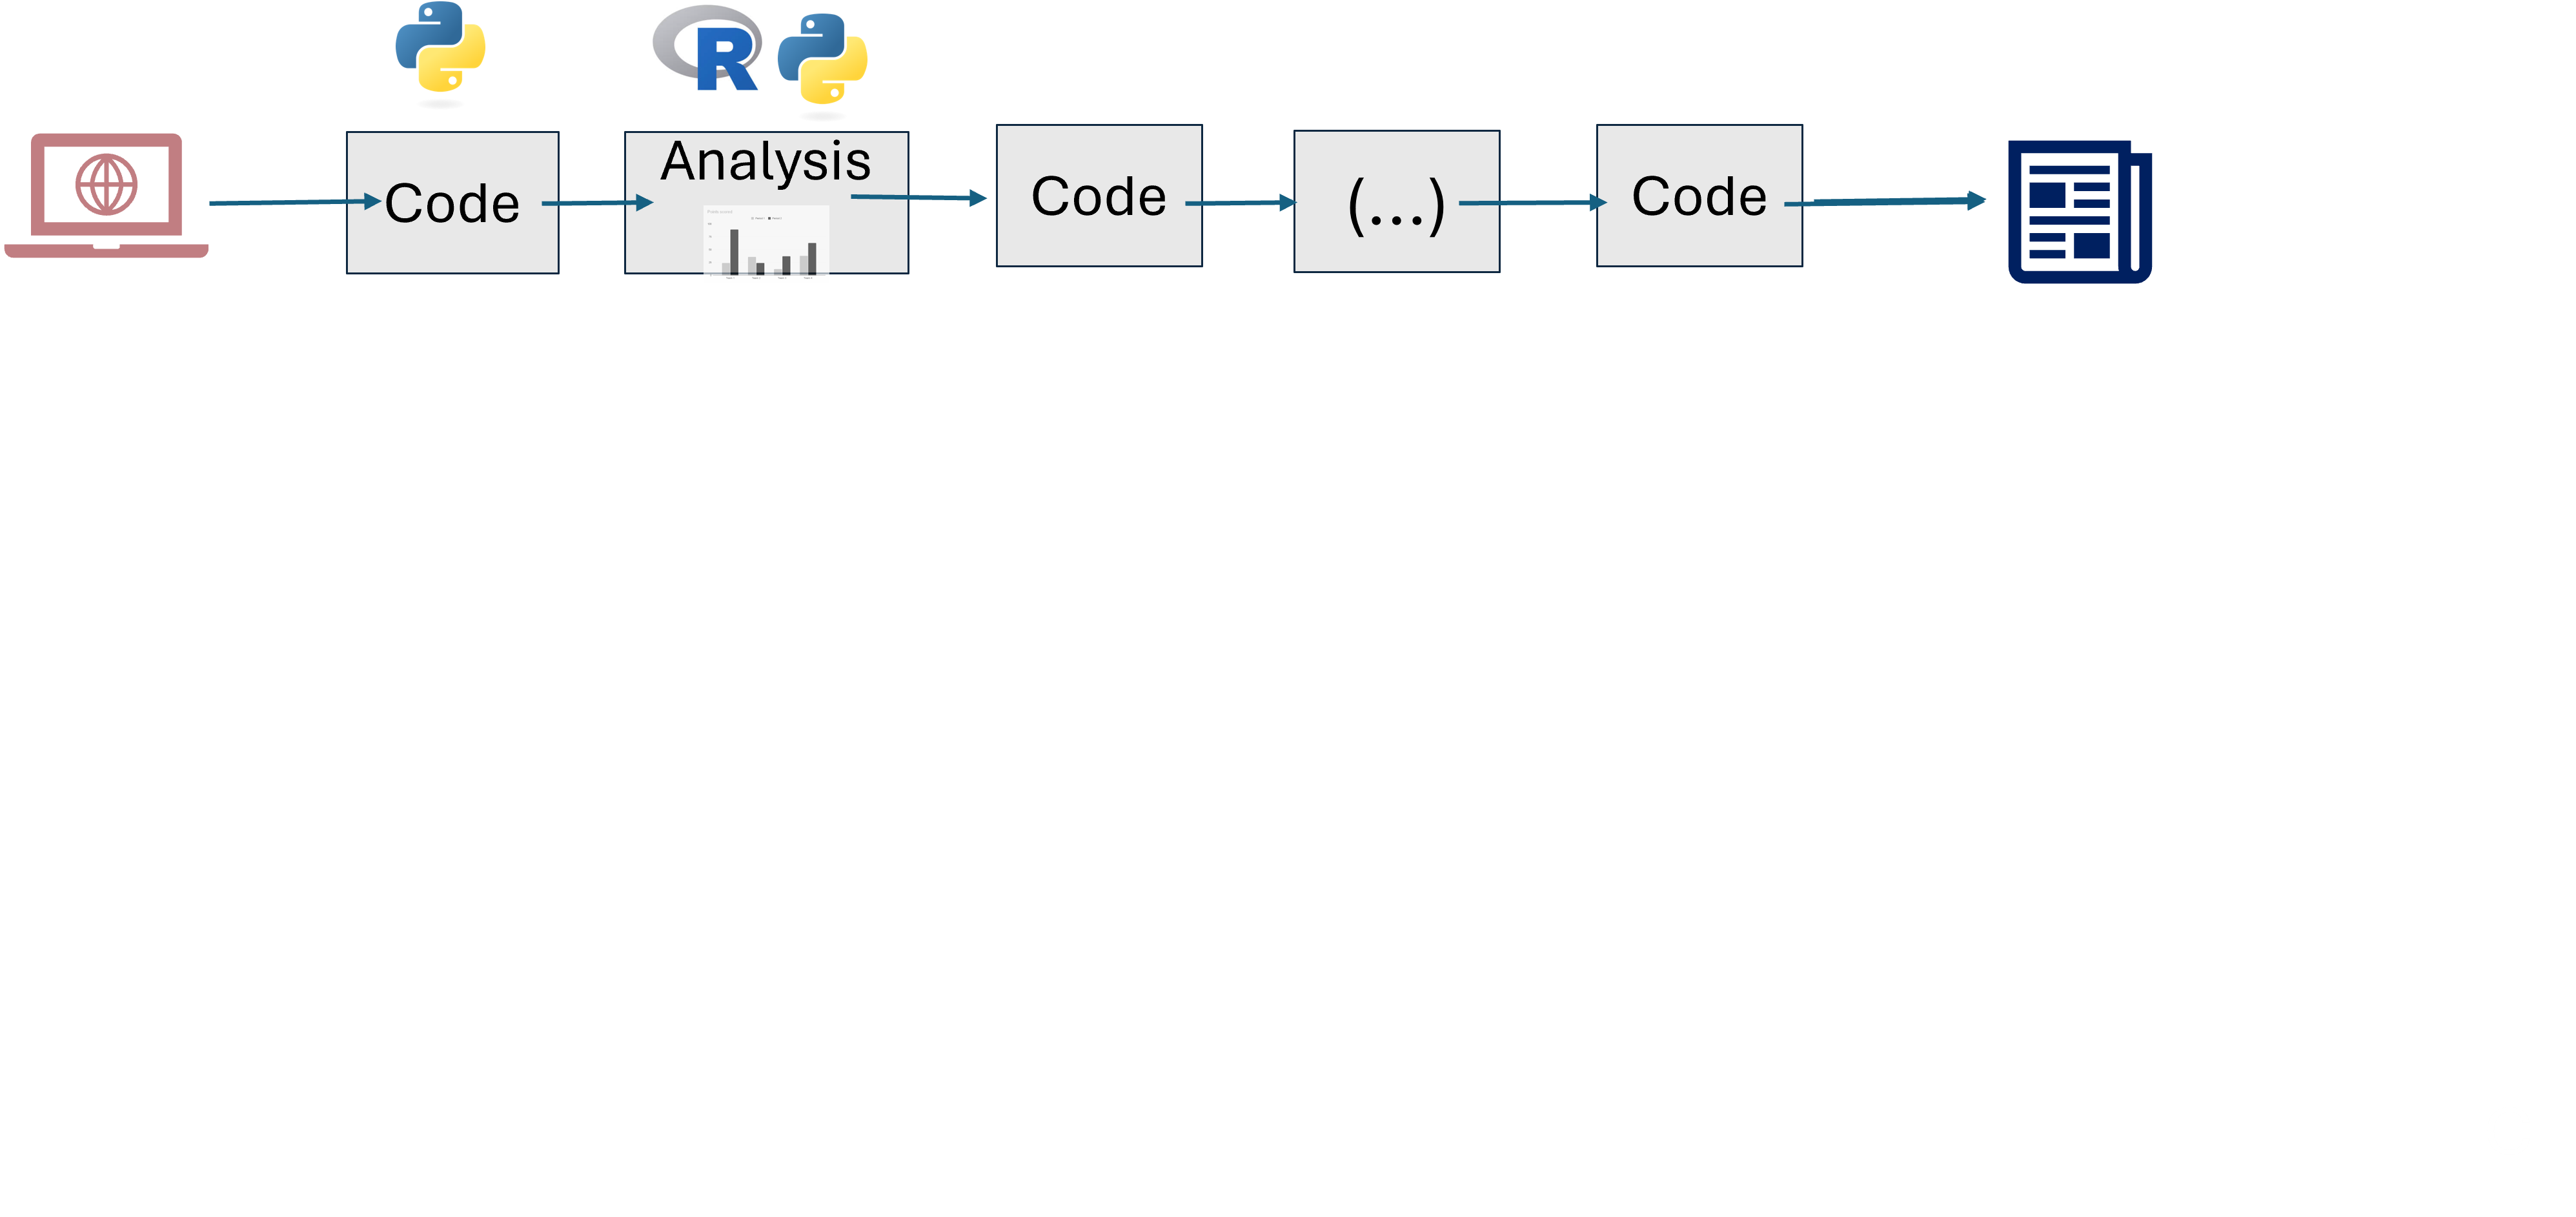
\includegraphics[width=0.8\textwidth]{Pipeline5.png} \\ Comment 5}
        \only<6>{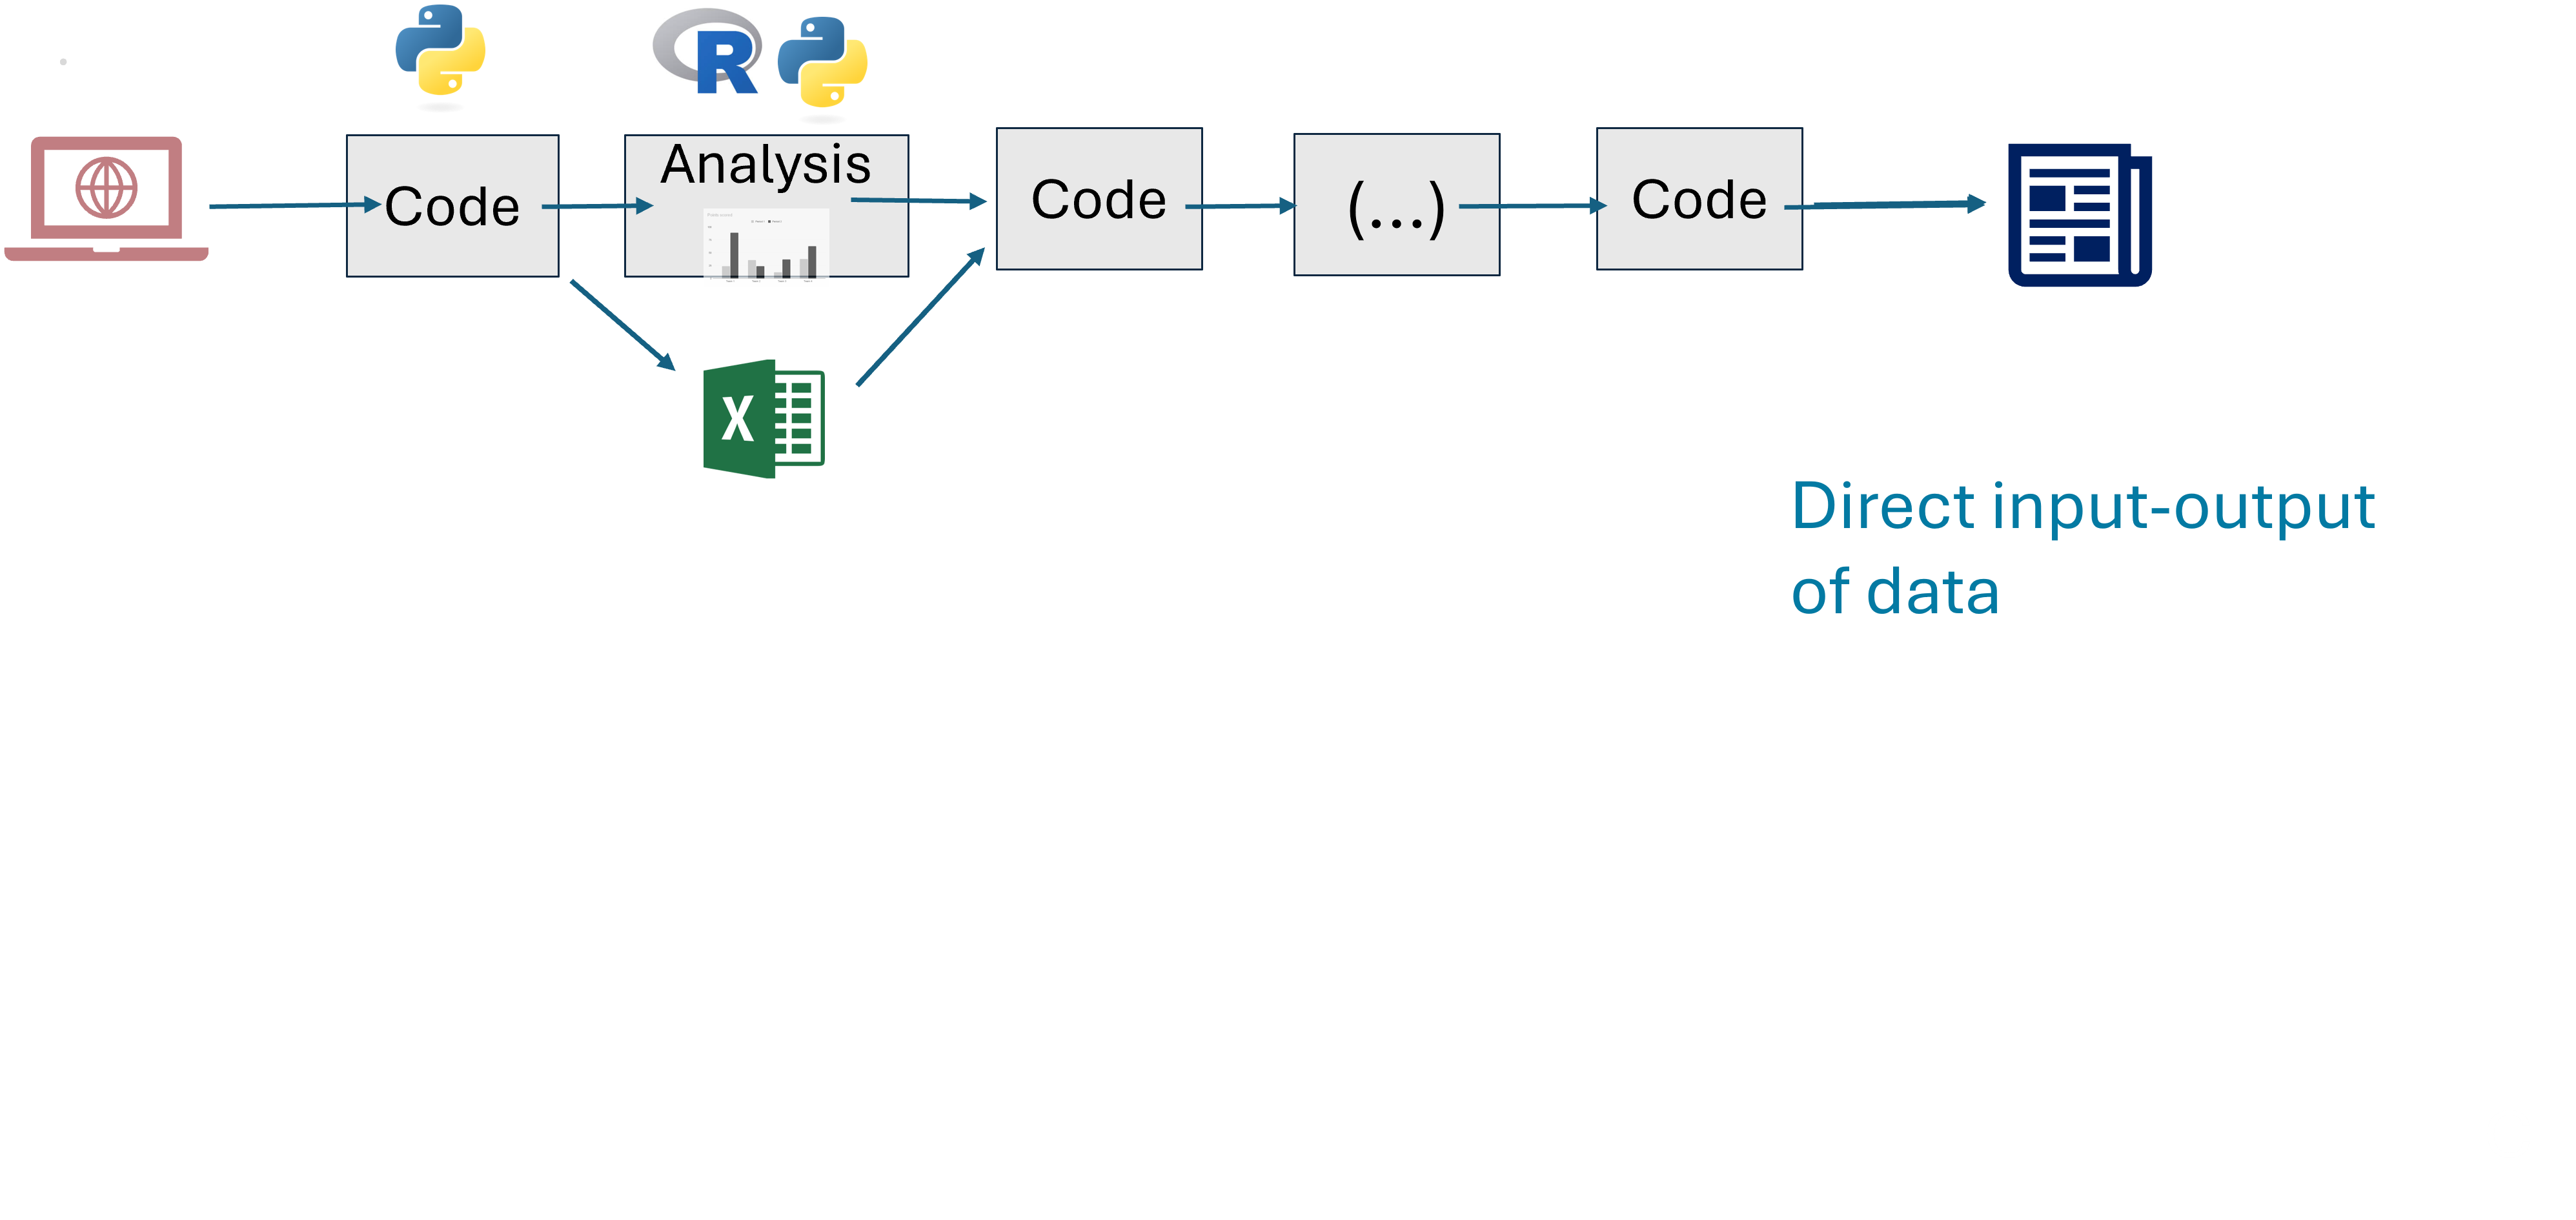
\includegraphics[width=0.8\textwidth]{Pipeline6.png} \\ Comment 6}
        \only<7>{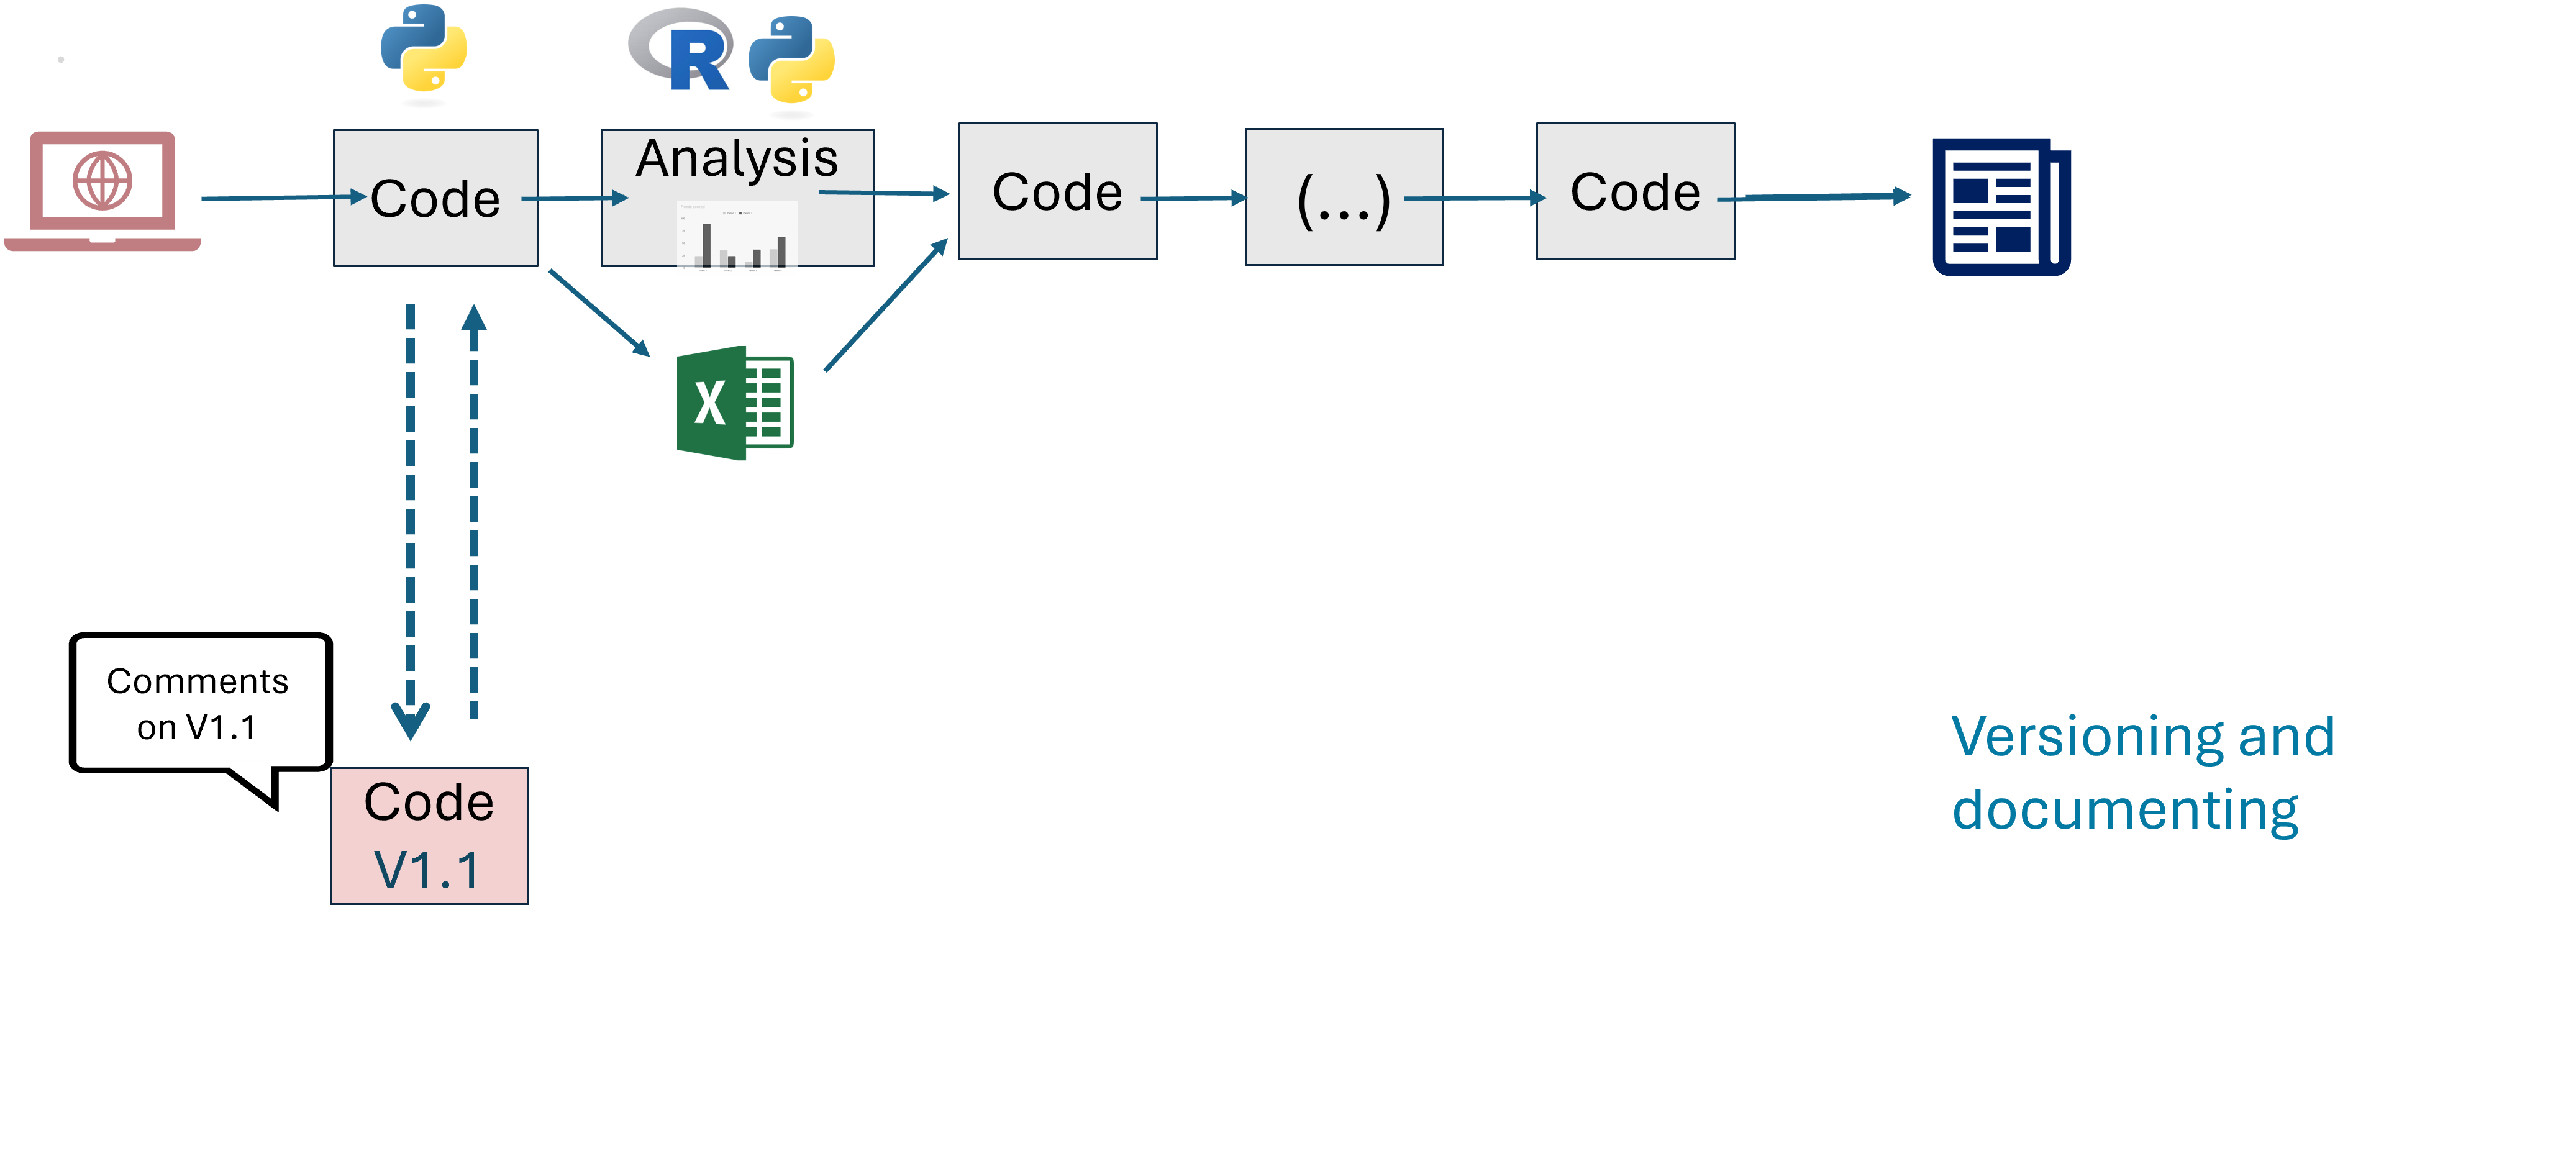
\includegraphics[width=0.8\textwidth]{Pipeline7.png} \\ Comment 7}
        \only<8>{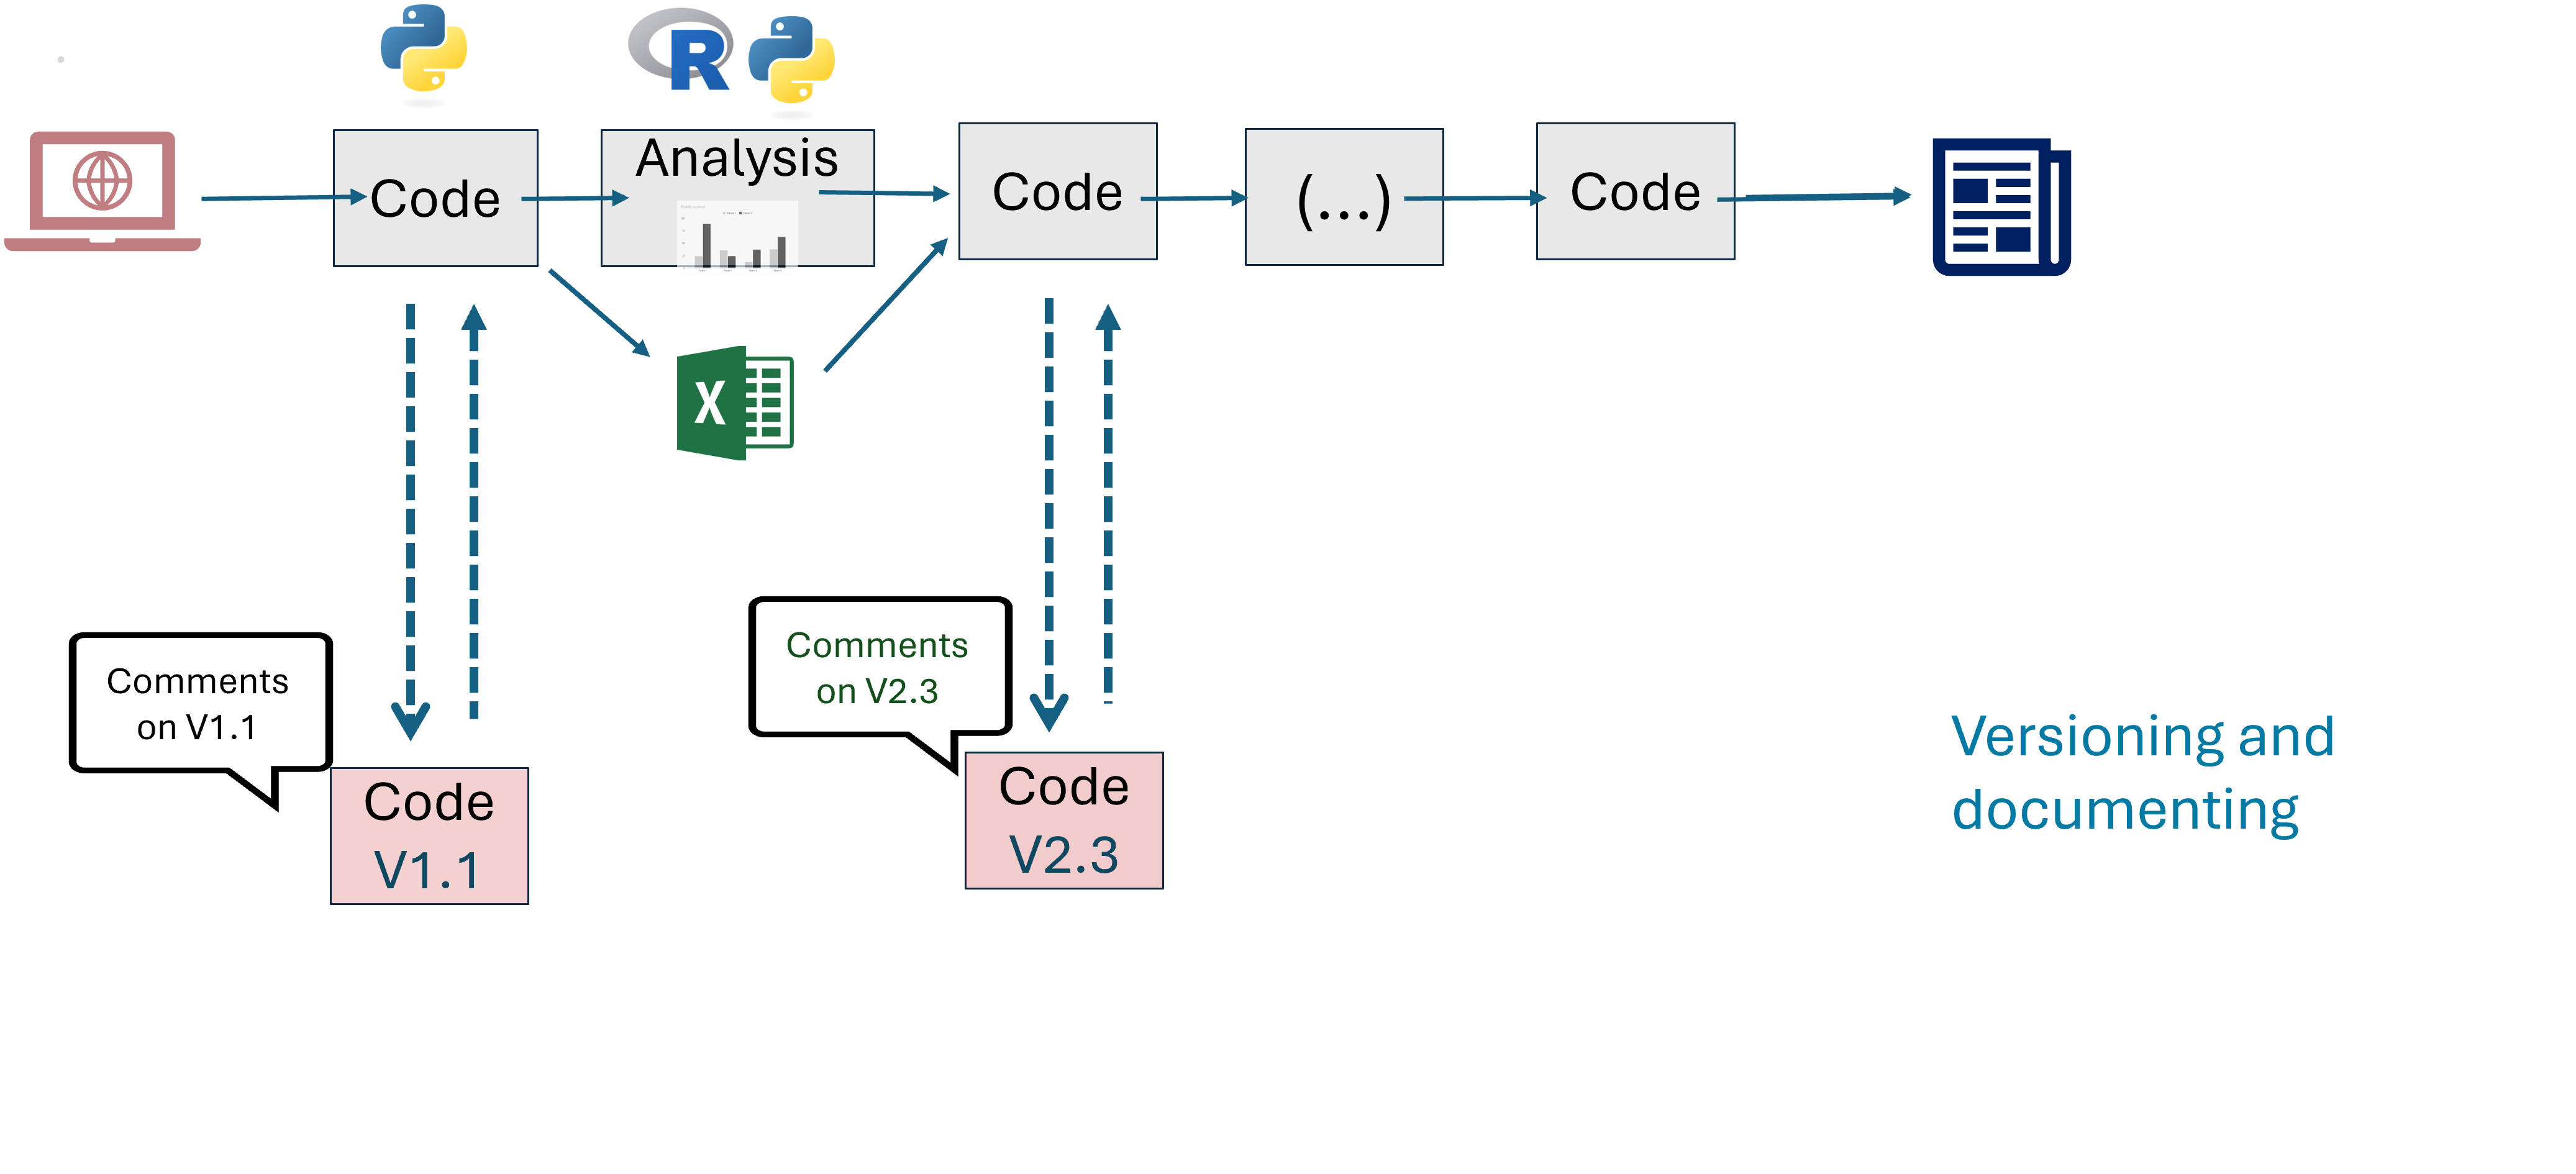
\includegraphics[width=0.8\textwidth]{Pipeline8.png} \\ Comment 8}
        \only<9>{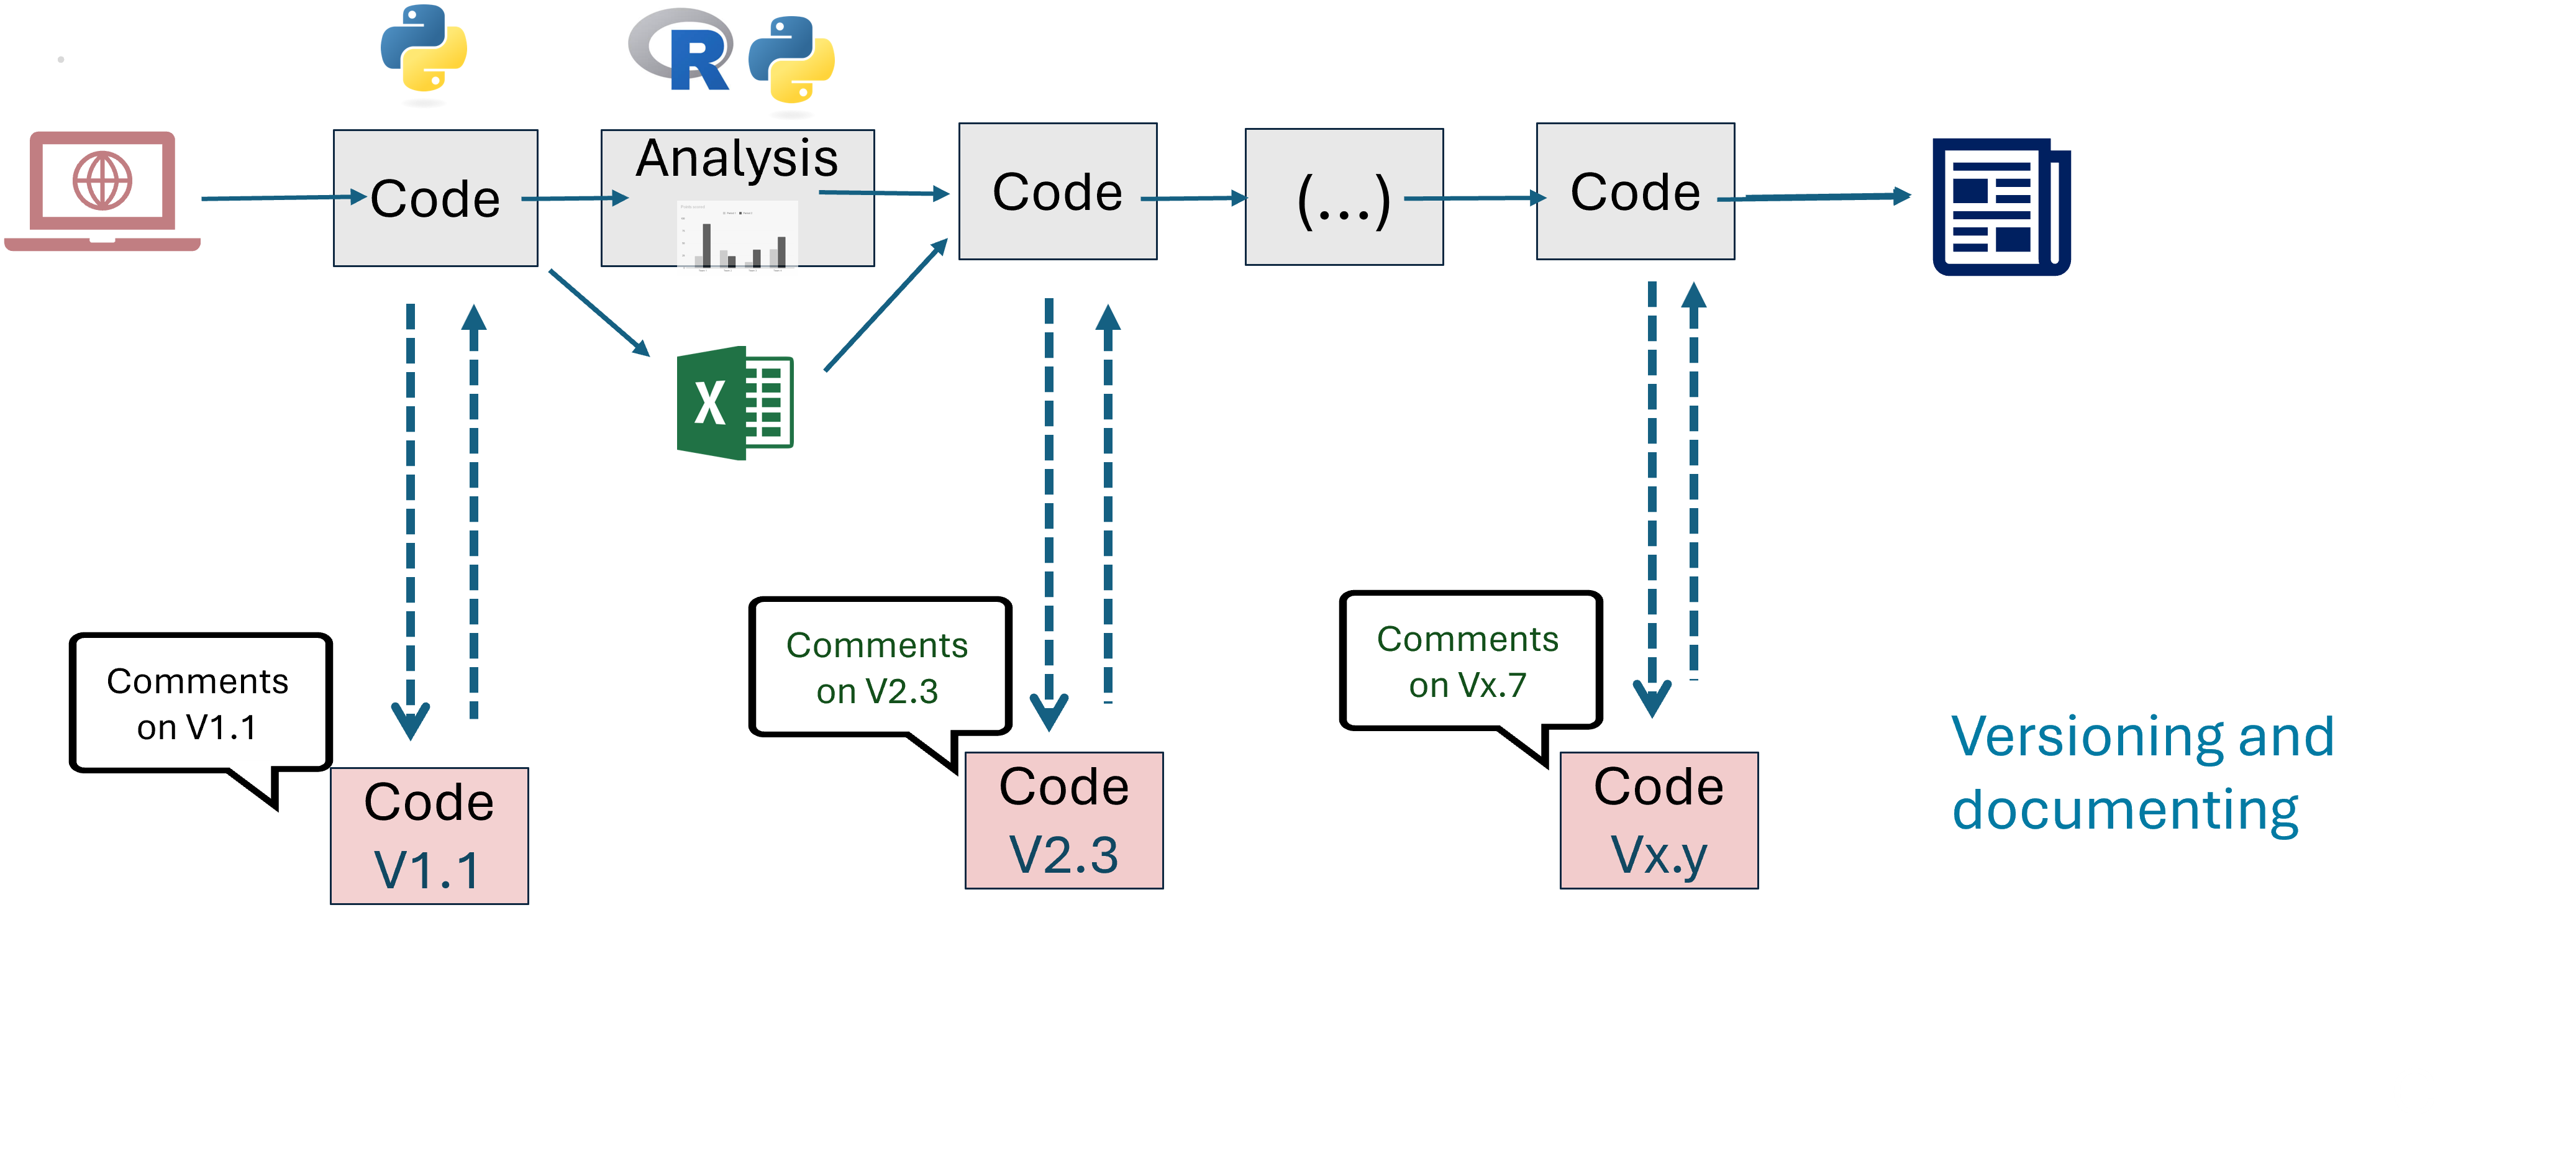
\includegraphics[width=0.8\textwidth]{Pipeline9.png} \\ Comment 9}
        \only<10>{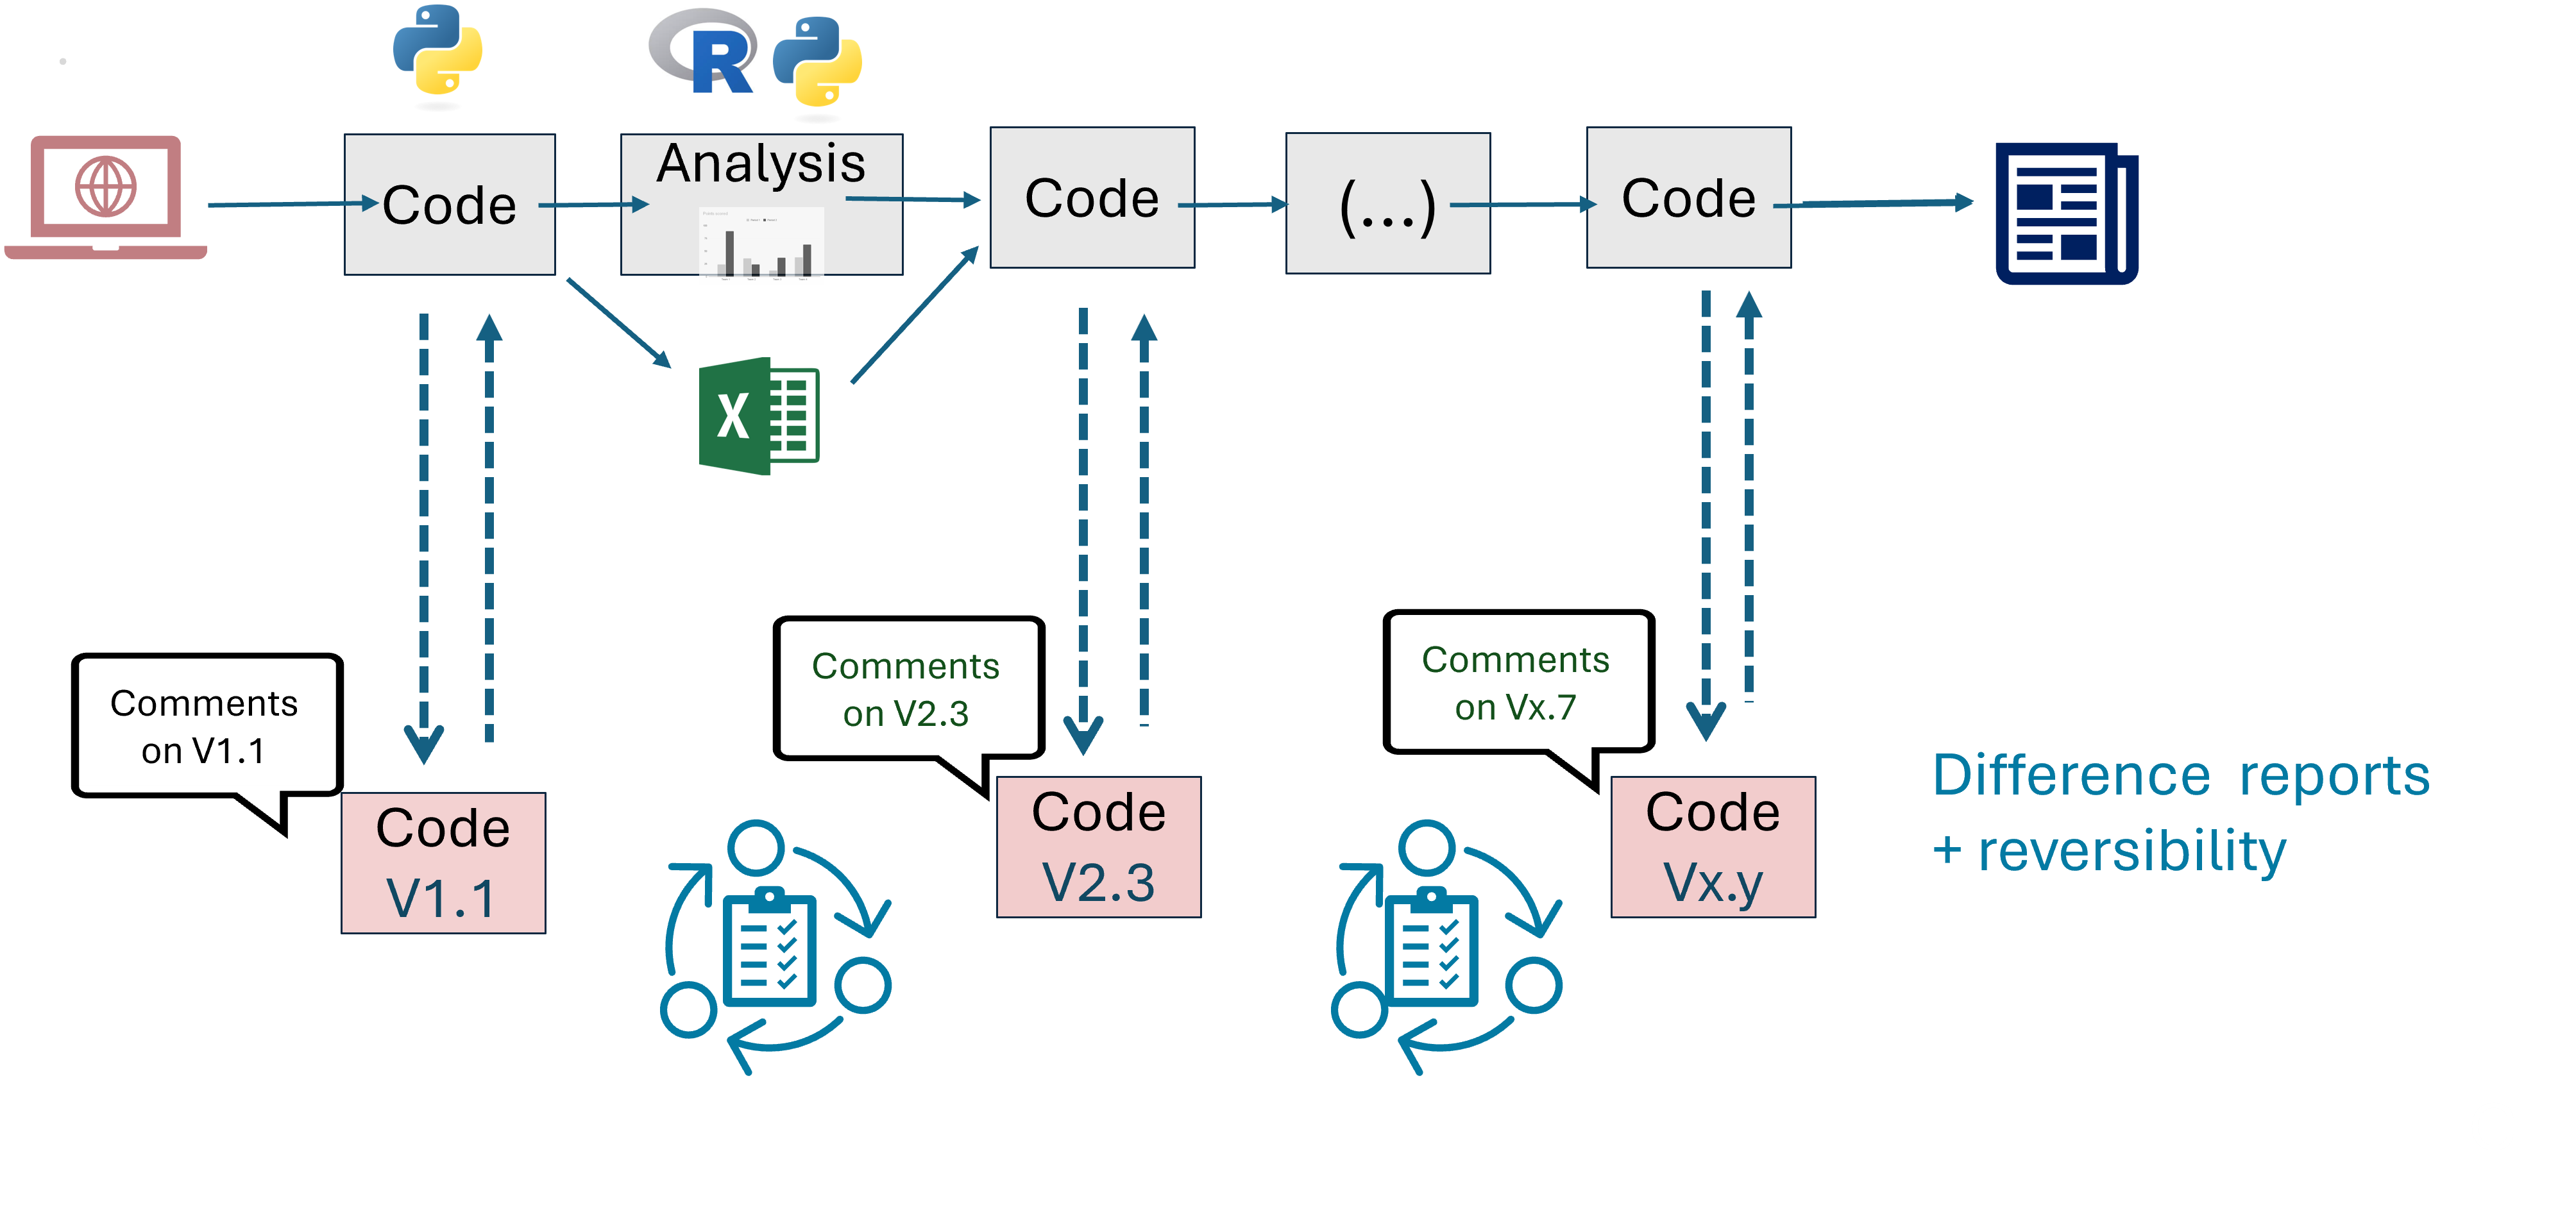
\includegraphics[width=0.8\textwidth]{Pipeline10.png} \\ Comment 10}
    \end{itemize}
\end{center}
\end{frame}


% Other slides go here...

\section{3 Principles}

\begin{frame}[<+->]
   \frametitle{3 main principles:}
    \begin{enumerate}
     \item Organize your work
     \item Code for others (including your future self)
     \item DRY: \textbf{D}o \textcolor{brique}{ not} \textbf{R}epeat \textbf{Y}ourself
      \item[]   \begin{alertblock}{}
            \begin{center}
                  \textit{Apply this in context (colleagues, code, software,...)}
            \end{center}
      \end{alertblock}
    \end{enumerate}
\end{frame}

\subsection{Organize your work }

\begin{frame}
\frametitle{Organize your work }
\textcolor{siap}{\textbf{Have a clear directory structure}}
 \pause
\begin{columns}[t]
 \begin{column}{0.4\textwidth}

    \begin{itemize}[<+->]
   \item Separate files into data, code, docs, etc. 
   \item Make directories portable\\ (relative path)
    \end{itemize}
\end{column}
  \begin{column}{0.6\textwidth}
    \begin{center}
    \begin{itemize}
         \only<2-4>{ 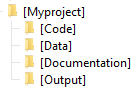
\includegraphics[width=0.5\textwidth]{WorkingDirectory.png} \\  }
         \only<2-4>{\hfill \tiny{ \textcolor{gris}{Example of a well-organized directory structure.}}\\ }
         \only<3-4>{\tiny{ \textbf{Usual}} \\ }
         \only<3-4>{ \tiny{mydata = pd.read\_csv("c://ESCAP/Webscraping/Data/WebData.csv")}  \\ \vspace{0.5cm} }
         \only<4>{\tiny{ \textbf{Better}}  \\}
         \only<4>{\tiny{\emph{Assuming your code is in } c://ESCAP/Webscraping/Code/ }  \\ }
         \only<4>{ \tiny{mydata = pd.read\_csv("../Data/WebData.csv")}  }

    \end{itemize}
    \end{center}
  \end{column}
\end{columns}
\end{frame}


\begin{frame}
\frametitle{Organize your work }
\textcolor{siap}{\textbf{Use naming conventions: } \\ }
For \textbf{files}\\
\begin{columns}[t]
 \begin{column}{0.3\textwidth}
    \begin{itemize}[<+->]
   \item Avoid  lazy names
   \item Meaningful files names
   \item Order of execution
    \end{itemize}
\end{column}
  \begin{column}{0.2\textwidth}
    \begin{itemize}
       \item[]
        \only<1-3>{ \small Usual \\ }
        \only<1-3>{ \small \texttt{prog1.ipynb}\\
                    \texttt{prog2.ipynb}\\
                    \texttt{Stat.ipynb}\\
                    \texttt{progC.ipynb}\\
                    \texttt{progP.ipynb} \\ }
    \end{itemize}
  \end{column}
  \begin{column}{0.5\textwidth}
    \begin{itemize}
        \item[]
        \only<2>{\small Better \\ }
        \only<2>{ \small    \texttt{Scraping\_Data.ipynb}\\
                            \texttt{Cleaning\_Data.ipynb}\\
                            \texttt{Stats\_Tables.ipynb}\\
                            \texttt{Classification.ipynb}\\
                            \texttt{Price\_CPI.ipynb} }
        \only<3>{\small Even better \\ }
        \only<3>{ \small
                    \texttt{01\_Scraping\_data.ipynb}\\   
                    \texttt{02\_Cleaning\_data.ipynb}\\
                    \texttt{03\_Classification.ipynb}\\
                    \texttt{04\_Stats\_Tables.ipynb}\\
                    \texttt{04\_Price\_CPI.ipynb} }

    \end{itemize}
  \end{column}
\end{columns}
\end{frame}


\begin{frame}
\frametitle{Organize your work }
\textcolor{siap}{\textbf{Use naming conventions:} \\ }
For \textbf{outputs}
\begin{columns}[t]
 \begin{column}{0.3\textwidth}
    \begin{itemize}[<+->]
   \item Avoid numbering
   \item Explicit type of output
    \end{itemize}
\end{column}
  \begin{column}{0.2\textwidth}
    \begin{itemize}
    \item[]
        \only<1-2>{\small Usual \\ }
        \only<1-2>{\small \texttt{Table1.pdf} \\
                    \texttt{Table2.pdf} \\
                    \texttt{Graph.jpg} \\
                    \texttt{Model.csv} \\ }
    \end{itemize}
  \end{column}
  \begin{column}{0.5\textwidth}
    \begin{itemize}
    \item[]
        \only<2>{\small Better \\ }
        \only<2>{ \small  \texttt{Stat\_Desc\_Table.pdf} \\
                    \texttt{Price\_Stat\_Table.pdf}\\
                    \texttt{Dress\_Prices\_Graphic.jpg}\\
                    \texttt{All\_prices\_Results.csv} \\ }
    \end{itemize}
  \end{column}
\end{columns}
\end{frame}


\begin{frame}
\frametitle{Organize your work }
\textcolor{siap}{\textbf{Keep track of the workflow:} \\  }
 \begin{columns}[t]
 \begin{column}{0.5\textwidth}
    \begin{itemize}[<+->]
     \item Cut and paste should be avoided
     \item Every step of the process is coded
     \item Manage (and draw) the workflow
   \end{itemize}
  \end{column}
 \begin{column}{0.5\textwidth}
    \begin{itemize}
        \item[]
        \only<1-3>{ \includegraphics[width=1.0\textwidth]{Workflow.png} \\ }
        \only<1-3>{\hfill \tiny{ \textcolor{gris}{Example of a simple workflow.}} }
    \end{itemize}
  \end{column}
\end{columns}
\end{frame}



\begin{frame}
\frametitle{Organize your work }
\textcolor{siap}{\textbf{Use a version control system  (Git/GitHub)}} \\
\vspace{0.5cm}
\begin{center}
 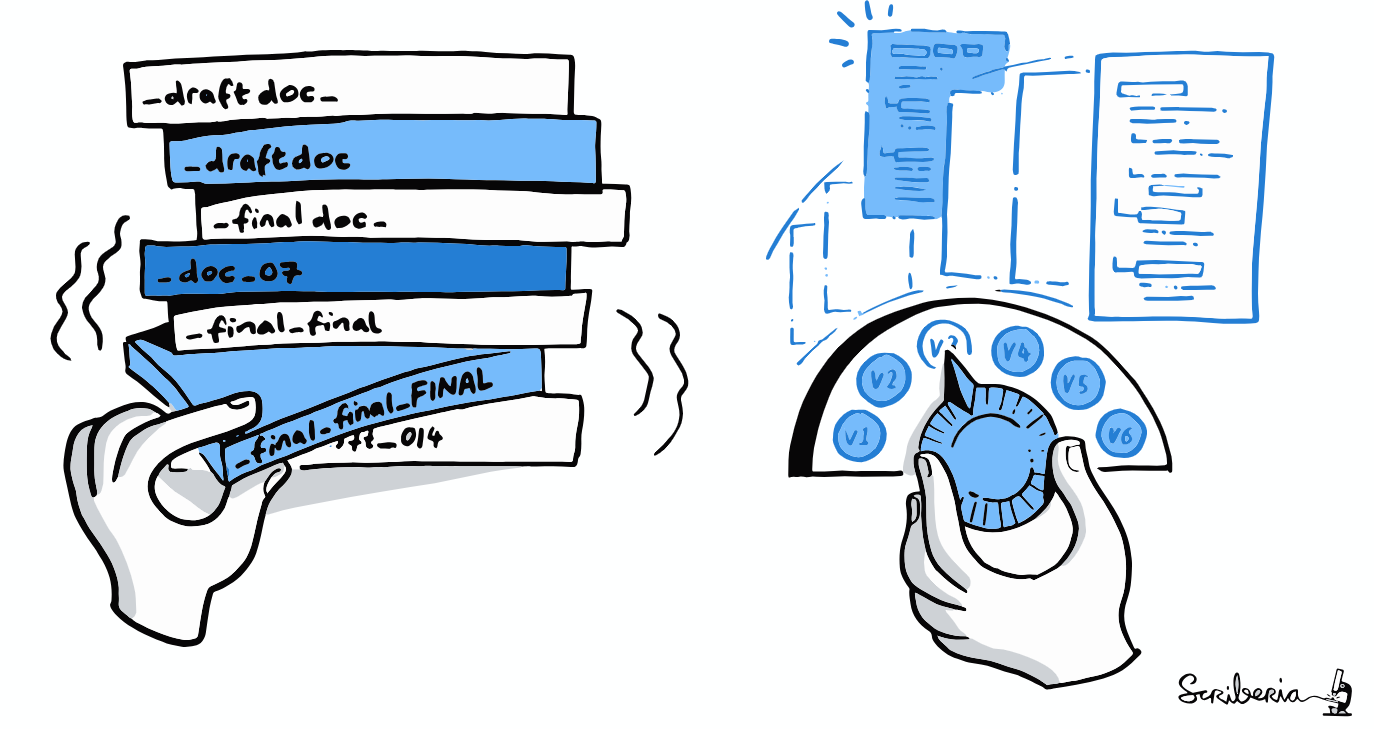
\includegraphics[width=0.7\textwidth]{FileHistory.PNG} \\
 
\large{\textbf{ More on Version Control later }}

\end{center}
\end{frame}

\subsection{Code for others}

\begin{frame}[<+->]
\frametitle{Code for others (including your "\emph{future self}")}
\textcolor{siap}{\textbf{Program with style:}} \\
          \begin{itemize}
             \item[]  \only<1>{Use \emph{literate programming} }
             \only<1>{ \begin{center}
                    ``\textit{Let us concentrate rather on explaining to humans \\ what we want the computer to do}'' \\
                    \hfill \textcolor{gris}{ D. Knuth (1984)} 
             \end{center}}
             \only<2>{ Use conventions on layout (Comments, indentation,...)  \\
             \href{https://peps.python.org/pep-0008/}{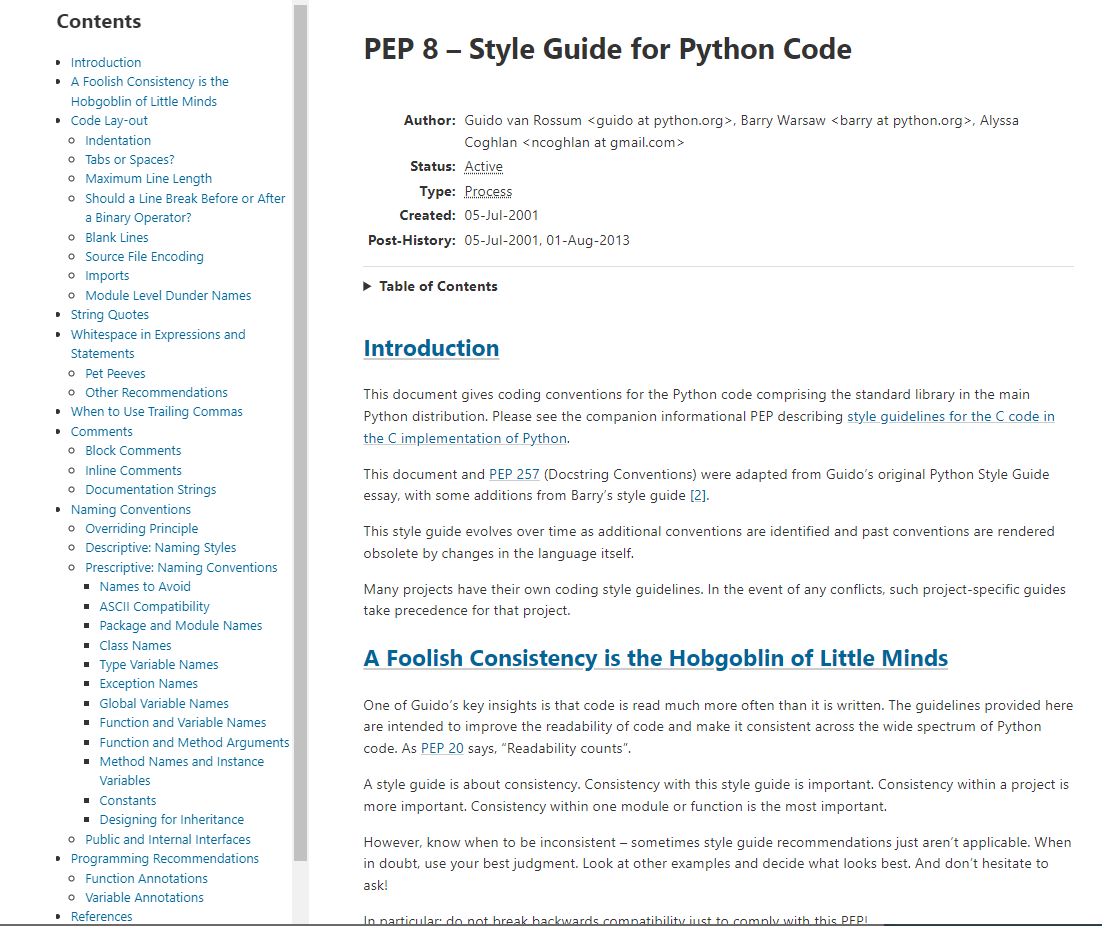
\includegraphics[width=0.8\textwidth]{PEP8-Style.png}}}
         \end{itemize}
\end{frame}


\begin{frame}
\frametitle{Code for others \textcolor[rgb]{1.00,0.00,0.00}{\textbf{<-- XXXX To revise this}} }
\textcolor{siap}{\textbf{Program with style}} \\
\begin{columns}[t]
 \begin{column}{0.3\textwidth}
    \begin{itemize}[<+->]
   \item Avoid ambiguities
   \item Avoid changing units
    \end{itemize}
\end{column}
  \begin{column}{0.7\textwidth}
    \begin{itemize}
    \item[]
        \only<1>{\scriptsize Usual \\ }
        \only<1>{\scriptsize \texttt{sex <- ifelse(gender == "1001", 1, 2)} \\}
        \only<1>{\small Better \\ }
        \only<1>{\scriptsize \texttt{female <- ifelse(gender == "1001",1,0)} \\
                                 \texttt{     male <- ifelse(gender != "1001",1,0)} \\ }
         \only<2-4>{\scriptsize Usual \\ }
        \only<2-4>{\scriptsize \texttt{gdp <- gdp/118.722 } \\
                                \texttt{ } \\ }
        \only<3>{\scriptsize Better \\ }
        \only<3>{\scriptsize \texttt{gdp\_US <- gdp / 118.722}  }
        \only<4>{\scriptsize Even better \\ }
        \only<4>{\scriptsize \texttt{US\_Vanu\_exch\_rate <- 118.722} \\
                                 \texttt{gdp\_US <- gdp / US\_Vanu\_exch\_rate}  }

    \end{itemize}
  \end{column}
\end{columns}
\end{frame}



%%%%%%
\subsection{DRY}
\begin{frame}
\frametitle{\textbf{D}o not \textbf{R}epeat \textbf{Y}ourself   \textcolor[rgb]{1.00,0.00,0.00}{\textbf{<--XXXX To revise this}} }

\textcolor{siap}{\textbf{Create reusable objects}} \\
\begin{columns}[t]
 \begin{column}{0.2\textwidth}
    \begin{itemize}[<+->]
       \item { \scriptsize Store values}
       \item[]
        \item { \scriptsize Avoid repetitions}
        \item[]
       \item { \scriptsize Use functions}
    \end{itemize}
\end{column}
  \begin{column}{0.8\textwidth}
    \begin{itemize}
    \item[]
        \only<1-2>{\scriptsize Usual \\ }
        \only<1-2>{\scriptsize \texttt{Current\_Data <- subset(Mydata, year  ==2023)} \\}
        \only<2>{\scriptsize Better \\ }
        \only<2>{\scriptsize \texttt{Current\_year <- 2023 \\
                        \texttt{Current\_Data <- subset(Mydata,} \\
                       \hfill \texttt{year == Current\_year)}} \\ }
        \only<3>{\scriptsize Usual \\ }
        \only<3>{\scriptsize \texttt{data <- Mydata[Mydata\$export == "Beef", ]} \\
                 \scriptsize \texttt{plot(data\$Year, data\$Value, } \\
                 \hfill \scriptsize \texttt{ main =  "Export for Beef") \\ }
                 \scriptsize \texttt{  } \\ }
        \only<3>{\scriptsize \texttt{data <- Mydata[Mydata\$export == "Kava", ]} \\
                \scriptsize \texttt{plot(data\$Year, data\$Value, } \\
                 \hfill \scriptsize \texttt{ main =  "Export for Kava") \\ }
                 \texttt{ ... } \\ }
        \only<4>{\scriptsize Better \\ }
        \only<4>{\scriptsize \texttt{ type <- "Beef"} \\
                                \texttt{ } \\
                                \texttt{  Mydata \%>\% } \\
                                \texttt{    filter(exports == type) \%>\%}\\
                                \texttt{    ggplot() + }\\
                                \texttt{    aes(x = Year, y = Value) +}\\
                                \texttt{    geom\_point() + }\\
                                \texttt{    ggtitle(paste("Export for ", type)) }\\
                                \texttt{ } \\ }
         \only<5>{\scriptsize Even better \\ }
         \only<5>{\scriptsize \texttt{Exports\_graphic <- function(type) \{ } \\
                                \texttt{  Mydata \%>\% } \\
                                \texttt{    filter(exports == type) \%>\%}\\
                                \texttt{    ggplot() + }\\
                                \texttt{    aes(x = Year, y = Value) +}\\
                                \texttt{    geom\_point() + }\\
                                \texttt{    ggtitle(paste("Export for ", type)) }\\
                                \texttt{\} }\\
                                \texttt{ } \\
                                \texttt{Exports\_graphic("Beef")} \\
                                \texttt{Exports\_graphic("Kava")   }}

    \end{itemize}
  \end{column}
\end{columns}
\end{frame}


\section{Version Control}








\section{Resources}
\begin{frame}{Useful resources}
  \begin{itemize}
    \item The UK government RAP \href{https://ukgovdatascience.github.io/rap-website/index.html}{website}.
    \item UK best practice \href{https://gss.civilservice.gov.uk/policy-store/quality-statistics-in-government/\#reproducible-analytical-pipelines-rap-}{documentation}.
    \item A free RAP \href{https://www.udemy.com/course/reproducible-analytical-pipelines/}{course} to teach you all you need to know.
    \item How the Data Science Campus sets its coding \href{https://datasciencecampus.github.io/coding-standards/}{standards}.
    \item A new open-source \href{https://the-turing-way.netlify.com}{book} from the Alan Turing institute setting out how to do reproducible data science.
  \end{itemize}
\end{frame}




\end{document}


